\documentclass[twoside]{book}

% Packages required by doxygen
\usepackage{fixltx2e}
\usepackage{calc}
\usepackage{doxygen}
\usepackage[export]{adjustbox} % also loads graphicx
\usepackage{graphicx}
\usepackage[utf8]{inputenc}
\usepackage{makeidx}
\usepackage{multicol}
\usepackage{multirow}
\PassOptionsToPackage{warn}{textcomp}
\usepackage{textcomp}
\usepackage[nointegrals]{wasysym}
\usepackage[table]{xcolor}

% Font selection
\usepackage[T1]{fontenc}
\usepackage[scaled=.90]{helvet}
\usepackage{courier}
\usepackage{amssymb}
\usepackage{sectsty}
\renewcommand{\familydefault}{\sfdefault}
\allsectionsfont{%
  \fontseries{bc}\selectfont%
  \color{darkgray}%
}
\renewcommand{\DoxyLabelFont}{%
  \fontseries{bc}\selectfont%
  \color{darkgray}%
}
\newcommand{\+}{\discretionary{\mbox{\scriptsize$\hookleftarrow$}}{}{}}

% Page & text layout
\usepackage{geometry}
\geometry{%
  a4paper,%
  top=2.5cm,%
  bottom=2.5cm,%
  left=2.5cm,%
  right=2.5cm%
}
\tolerance=750
\hfuzz=15pt
\hbadness=750
\setlength{\emergencystretch}{15pt}
\setlength{\parindent}{0cm}
\setlength{\parskip}{3ex plus 2ex minus 2ex}
\makeatletter
\renewcommand{\paragraph}{%
  \@startsection{paragraph}{4}{0ex}{-1.0ex}{1.0ex}{%
    \normalfont\normalsize\bfseries\SS@parafont%
  }%
}
\renewcommand{\subparagraph}{%
  \@startsection{subparagraph}{5}{0ex}{-1.0ex}{1.0ex}{%
    \normalfont\normalsize\bfseries\SS@subparafont%
  }%
}
\makeatother

% Headers & footers
\usepackage{fancyhdr}
\pagestyle{fancyplain}
\fancyhead[LE]{\fancyplain{}{\bfseries\thepage}}
\fancyhead[CE]{\fancyplain{}{}}
\fancyhead[RE]{\fancyplain{}{\bfseries\leftmark}}
\fancyhead[LO]{\fancyplain{}{\bfseries\rightmark}}
\fancyhead[CO]{\fancyplain{}{}}
\fancyhead[RO]{\fancyplain{}{\bfseries\thepage}}
\fancyfoot[LE]{\fancyplain{}{}}
\fancyfoot[CE]{\fancyplain{}{}}
\fancyfoot[RE]{\fancyplain{}{\bfseries\scriptsize Generated by Doxygen }}
\fancyfoot[LO]{\fancyplain{}{\bfseries\scriptsize Generated by Doxygen }}
\fancyfoot[CO]{\fancyplain{}{}}
\fancyfoot[RO]{\fancyplain{}{}}
\renewcommand{\footrulewidth}{0.4pt}
\renewcommand{\chaptermark}[1]{%
  \markboth{#1}{}%
}
\renewcommand{\sectionmark}[1]{%
  \markright{\thesection\ #1}%
}

% Indices & bibliography
\usepackage{natbib}
\usepackage[titles]{tocloft}
\setcounter{tocdepth}{3}
\setcounter{secnumdepth}{5}
\makeindex

% Hyperlinks (required, but should be loaded last)
\usepackage{ifpdf}
\ifpdf
  \usepackage[pdftex,pagebackref=true]{hyperref}
\else
  \usepackage[ps2pdf,pagebackref=true]{hyperref}
\fi
\hypersetup{%
  colorlinks=true,%
  linkcolor=blue,%
  citecolor=blue,%
  unicode%
}

% Custom commands
\newcommand{\clearemptydoublepage}{%
  \newpage{\pagestyle{empty}\cleardoublepage}%
}

\usepackage{caption}
\captionsetup{labelsep=space,justification=centering,font={bf},singlelinecheck=off,skip=4pt,position=top}

%===== C O N T E N T S =====

\begin{document}

% Titlepage & ToC
\hypersetup{pageanchor=false,
             bookmarksnumbered=true,
             pdfencoding=unicode
            }
\pagenumbering{alph}
\begin{titlepage}
\vspace*{7cm}
\begin{center}%
{\Large Overflow }\\
\vspace*{1cm}
{\large Generated by Doxygen 1.8.12}\\
\end{center}
\end{titlepage}
\clearemptydoublepage
\pagenumbering{roman}
\tableofcontents
\clearemptydoublepage
\pagenumbering{arabic}
\hypersetup{pageanchor=true}

%--- Begin generated contents ---
\chapter{Namespace Index}
\section{Namespace List}
Here is a list of all namespaces with brief descriptions\+:\begin{DoxyCompactList}
\item\contentsline{section}{\hyperlink{namespace_collections}{Collections} }{\pageref{namespace_collections}}{}
\item\contentsline{section}{\hyperlink{namespace_error}{Error} }{\pageref{namespace_error}}{}
\item\contentsline{section}{\hyperlink{namespace_error_1_1_error_code}{Error\+::\+Error\+Code} }{\pageref{namespace_error_1_1_error_code}}{}
\item\contentsline{section}{\hyperlink{namespace_flow}{Flow} }{\pageref{namespace_flow}}{}
\item\contentsline{section}{\hyperlink{namespace_flow_1_1_diff}{Flow\+::\+Diff} }{\pageref{namespace_flow_1_1_diff}}{}
\item\contentsline{section}{\hyperlink{namespace_flow_1_1_direct}{Flow\+::\+Direct} }{\pageref{namespace_flow_1_1_direct}}{}
\item\contentsline{section}{\hyperlink{namespace_flow_1_1_dmg_elem}{Flow\+::\+Dmg\+Elem} }{\pageref{namespace_flow_1_1_dmg_elem}}{}
\end{DoxyCompactList}

\chapter{Hierarchical Index}
\section{Class Hierarchy}
This inheritance list is sorted roughly, but not completely, alphabetically\+:\begin{DoxyCompactList}
\item \contentsline{section}{Flow\+:\+:Actor}{\pageref{class_flow_1_1_actor}}{}
\item \contentsline{section}{Flow\+:\+:Bin\+Array}{\pageref{class_flow_1_1_bin_array}}{}
\item \contentsline{section}{Flow\+:\+:Config}{\pageref{struct_flow_1_1_config}}{}
\item \contentsline{section}{Flow\+:\+:Flg\+Util}{\pageref{class_flow_1_1_flg_util}}{}
\item \contentsline{section}{Flow\+:\+:Floor}{\pageref{class_flow_1_1_floor}}{}
\item \contentsline{section}{Flow\+:\+:Game}{\pageref{struct_flow_1_1_game}}{}
\item \contentsline{section}{Flow\+:\+:Gm\+Rand}{\pageref{class_flow_1_1_gm_rand}}{}
\item \contentsline{section}{Flow\+:\+:Item}{\pageref{class_flow_1_1_item}}{}
\item \contentsline{section}{Flow\+:\+:Point}{\pageref{struct_flow_1_1_point}}{}
\item \contentsline{section}{Flow\+:\+:Room}{\pageref{class_flow_1_1_room}}{}
\item \contentsline{section}{Flow\+:\+:Stat}{\pageref{class_flow_1_1_stat}}{}
\begin{DoxyCompactList}
\item \contentsline{section}{Flow\+:\+:B\+Stat}{\pageref{class_flow_1_1_b_stat}}{}
\item \contentsline{section}{Flow\+:\+:I\+Stat}{\pageref{class_flow_1_1_i_stat}}{}
\end{DoxyCompactList}
\end{DoxyCompactList}

\chapter{Class Index}
\section{Class List}
Here are the classes, structs, unions and interfaces with brief descriptions\+:\begin{DoxyCompactList}
\item\contentsline{section}{\hyperlink{class_flow_1_1_actor}{Flow\+::\+Actor} }{\pageref{class_flow_1_1_actor}}{}
\item\contentsline{section}{\hyperlink{class_flow_1_1_bin_array}{Flow\+::\+Bin\+Array} }{\pageref{class_flow_1_1_bin_array}}{}
\item\contentsline{section}{\hyperlink{class_flow_1_1_b_stat}{Flow\+::\+B\+Stat} }{\pageref{class_flow_1_1_b_stat}}{}
\item\contentsline{section}{\hyperlink{struct_flow_1_1_config}{Flow\+::\+Config} }{\pageref{struct_flow_1_1_config}}{}
\item\contentsline{section}{\hyperlink{class_flow_1_1_flg_util}{Flow\+::\+Flg\+Util} }{\pageref{class_flow_1_1_flg_util}}{}
\item\contentsline{section}{\hyperlink{class_flow_1_1_floor}{Flow\+::\+Floor} }{\pageref{class_flow_1_1_floor}}{}
\item\contentsline{section}{\hyperlink{struct_flow_1_1_game}{Flow\+::\+Game} }{\pageref{struct_flow_1_1_game}}{}
\item\contentsline{section}{\hyperlink{class_flow_1_1_gm_rand}{Flow\+::\+Gm\+Rand} }{\pageref{class_flow_1_1_gm_rand}}{}
\item\contentsline{section}{\hyperlink{class_flow_1_1_i_stat}{Flow\+::\+I\+Stat} }{\pageref{class_flow_1_1_i_stat}}{}
\item\contentsline{section}{\hyperlink{class_flow_1_1_item}{Flow\+::\+Item} }{\pageref{class_flow_1_1_item}}{}
\item\contentsline{section}{\hyperlink{struct_flow_1_1_point}{Flow\+::\+Point} }{\pageref{struct_flow_1_1_point}}{}
\item\contentsline{section}{\hyperlink{class_flow_1_1_room}{Flow\+::\+Room} }{\pageref{class_flow_1_1_room}}{}
\item\contentsline{section}{\hyperlink{class_flow_1_1_stat}{Flow\+::\+Stat} }{\pageref{class_flow_1_1_stat}}{}
\end{DoxyCompactList}

\chapter{File Index}
\section{File List}
Here is a list of all files with brief descriptions\+:\begin{DoxyCompactList}
\item\contentsline{section}{Rothman\+Alexander\+\_\+\+C\+S\+C17\+A\+\_\+48096/proj/\+Project\+\_\+2/\+Overflow\+\_\+2/\hyperlink{_8dep_8inc}{.\+dep.\+inc} }{\pageref{_8dep_8inc}}{}
\item\contentsline{section}{Rothman\+Alexander\+\_\+\+C\+S\+C17\+A\+\_\+48096/proj/\+Project\+\_\+2/\+Overflow\+\_\+2/\hyperlink{actor_8cpp}{actor.\+cpp} }{\pageref{actor_8cpp}}{}
\item\contentsline{section}{Rothman\+Alexander\+\_\+\+C\+S\+C17\+A\+\_\+48096/proj/\+Project\+\_\+2/\+Overflow\+\_\+2/\hyperlink{actor_8h}{actor.\+h} }{\pageref{actor_8h}}{}
\item\contentsline{section}{Rothman\+Alexander\+\_\+\+C\+S\+C17\+A\+\_\+48096/proj/\+Project\+\_\+2/\+Overflow\+\_\+2/\hyperlink{collections_8h}{collections.\+h} }{\pageref{collections_8h}}{}
\item\contentsline{section}{Rothman\+Alexander\+\_\+\+C\+S\+C17\+A\+\_\+48096/proj/\+Project\+\_\+2/\+Overflow\+\_\+2/\hyperlink{enums_8h}{enums.\+h} }{\pageref{enums_8h}}{}
\item\contentsline{section}{Rothman\+Alexander\+\_\+\+C\+S\+C17\+A\+\_\+48096/proj/\+Project\+\_\+2/\+Overflow\+\_\+2/\hyperlink{except_8cpp}{except.\+cpp} }{\pageref{except_8cpp}}{}
\item\contentsline{section}{Rothman\+Alexander\+\_\+\+C\+S\+C17\+A\+\_\+48096/proj/\+Project\+\_\+2/\+Overflow\+\_\+2/\hyperlink{except_8h}{except.\+h} }{\pageref{except_8h}}{}
\item\contentsline{section}{Rothman\+Alexander\+\_\+\+C\+S\+C17\+A\+\_\+48096/proj/\+Project\+\_\+2/\+Overflow\+\_\+2/\hyperlink{flags_8cpp}{flags.\+cpp} }{\pageref{flags_8cpp}}{}
\item\contentsline{section}{Rothman\+Alexander\+\_\+\+C\+S\+C17\+A\+\_\+48096/proj/\+Project\+\_\+2/\+Overflow\+\_\+2/\hyperlink{flags_8h}{flags.\+h} }{\pageref{flags_8h}}{}
\item\contentsline{section}{Rothman\+Alexander\+\_\+\+C\+S\+C17\+A\+\_\+48096/proj/\+Project\+\_\+2/\+Overflow\+\_\+2/\hyperlink{functions_8cpp}{functions.\+cpp} }{\pageref{functions_8cpp}}{}
\item\contentsline{section}{Rothman\+Alexander\+\_\+\+C\+S\+C17\+A\+\_\+48096/proj/\+Project\+\_\+2/\+Overflow\+\_\+2/\hyperlink{functions_8h}{functions.\+h} }{\pageref{functions_8h}}{}
\item\contentsline{section}{Rothman\+Alexander\+\_\+\+C\+S\+C17\+A\+\_\+48096/proj/\+Project\+\_\+2/\+Overflow\+\_\+2/\hyperlink{game_8cpp}{game.\+cpp} }{\pageref{game_8cpp}}{}
\item\contentsline{section}{Rothman\+Alexander\+\_\+\+C\+S\+C17\+A\+\_\+48096/proj/\+Project\+\_\+2/\+Overflow\+\_\+2/\hyperlink{game_8h}{game.\+h} }{\pageref{game_8h}}{}
\item\contentsline{section}{Rothman\+Alexander\+\_\+\+C\+S\+C17\+A\+\_\+48096/proj/\+Project\+\_\+2/\+Overflow\+\_\+2/\hyperlink{item_8cpp}{item.\+cpp} }{\pageref{item_8cpp}}{}
\item\contentsline{section}{Rothman\+Alexander\+\_\+\+C\+S\+C17\+A\+\_\+48096/proj/\+Project\+\_\+2/\+Overflow\+\_\+2/\hyperlink{item_8h}{item.\+h} }{\pageref{item_8h}}{}
\item\contentsline{section}{Rothman\+Alexander\+\_\+\+C\+S\+C17\+A\+\_\+48096/proj/\+Project\+\_\+2/\+Overflow\+\_\+2/\hyperlink{macros_8h}{macros.\+h} }{\pageref{macros_8h}}{}
\item\contentsline{section}{Rothman\+Alexander\+\_\+\+C\+S\+C17\+A\+\_\+48096/proj/\+Project\+\_\+2/\+Overflow\+\_\+2/\hyperlink{main_8cpp}{main.\+cpp} }{\pageref{main_8cpp}}{}
\item\contentsline{section}{Rothman\+Alexander\+\_\+\+C\+S\+C17\+A\+\_\+48096/proj/\+Project\+\_\+2/\+Overflow\+\_\+2/\hyperlink{random_8cpp}{random.\+cpp} }{\pageref{random_8cpp}}{}
\item\contentsline{section}{Rothman\+Alexander\+\_\+\+C\+S\+C17\+A\+\_\+48096/proj/\+Project\+\_\+2/\+Overflow\+\_\+2/\hyperlink{random_8h}{random.\+h} }{\pageref{random_8h}}{}
\item\contentsline{section}{Rothman\+Alexander\+\_\+\+C\+S\+C17\+A\+\_\+48096/proj/\+Project\+\_\+2/\+Overflow\+\_\+2/\hyperlink{room_8cpp}{room.\+cpp} }{\pageref{room_8cpp}}{}
\item\contentsline{section}{Rothman\+Alexander\+\_\+\+C\+S\+C17\+A\+\_\+48096/proj/\+Project\+\_\+2/\+Overflow\+\_\+2/\hyperlink{room_8h}{room.\+h} }{\pageref{room_8h}}{}
\item\contentsline{section}{Rothman\+Alexander\+\_\+\+C\+S\+C17\+A\+\_\+48096/proj/\+Project\+\_\+2/\+Overflow\+\_\+2/\hyperlink{stat_8cpp}{stat.\+cpp} }{\pageref{stat_8cpp}}{}
\item\contentsline{section}{Rothman\+Alexander\+\_\+\+C\+S\+C17\+A\+\_\+48096/proj/\+Project\+\_\+2/\+Overflow\+\_\+2/\hyperlink{stat_8h}{stat.\+h} }{\pageref{stat_8h}}{}
\item\contentsline{section}{Rothman\+Alexander\+\_\+\+C\+S\+C17\+A\+\_\+48096/proj/\+Project\+\_\+2/\+Overflow\+\_\+2/\hyperlink{stringext_8cpp}{stringext.\+cpp} }{\pageref{stringext_8cpp}}{}
\item\contentsline{section}{Rothman\+Alexander\+\_\+\+C\+S\+C17\+A\+\_\+48096/proj/\+Project\+\_\+2/\+Overflow\+\_\+2/\hyperlink{stringext_8h}{stringext.\+h} }{\pageref{stringext_8h}}{}
\item\contentsline{section}{Rothman\+Alexander\+\_\+\+C\+S\+C17\+A\+\_\+48096/proj/\+Project\+\_\+2/\+Overflow\+\_\+2/\hyperlink{structs_8h}{structs.\+h} }{\pageref{structs_8h}}{}
\end{DoxyCompactList}

\chapter{Namespace Documentation}
\hypertarget{namespace_flow}{}\section{Flow Namespace Reference}
\label{namespace_flow}\index{Flow@{Flow}}
\subsection*{Namespaces}
\begin{DoxyCompactItemize}
\item 
 \hyperlink{namespace_flow_1_1_diff}{Diff}
\item 
 \hyperlink{namespace_flow_1_1_direct}{Direct}
\item 
 \hyperlink{namespace_flow_1_1_dmg_elem}{Dmg\+Elem}
\end{DoxyCompactItemize}
\subsection*{Classes}
\begin{DoxyCompactItemize}
\item 
class \hyperlink{class_flow_1_1_actor}{Actor}
\item 
class \hyperlink{class_flow_1_1_armor}{Armor}
\item 
class \hyperlink{class_flow_1_1_b_stat}{B\+Stat}
\item 
struct \hyperlink{struct_flow_1_1_config}{Config}
\item 
class \hyperlink{class_flow_1_1_flag_util}{Flag\+Util}
\item 
class \hyperlink{class_flow_1_1_floor}{Floor}
\item 
class \hyperlink{class_flow_1_1_game}{Game}
\item 
class \hyperlink{class_flow_1_1_gm_rand}{Gm\+Rand}
\item 
class \hyperlink{class_flow_1_1_i_stat}{I\+Stat}
\item 
class \hyperlink{class_flow_1_1_item}{Item}
\item 
struct \hyperlink{struct_flow_1_1_point}{Point}
\item 
class \hyperlink{class_flow_1_1_potion}{Potion}
\item 
struct \hyperlink{struct_flow_1_1_r_n_g_point}{R\+N\+G\+Point}
\item 
class \hyperlink{class_flow_1_1_room}{Room}
\item 
class \hyperlink{class_flow_1_1_stat}{Stat}
\item 
class \hyperlink{class_flow_1_1_weapon}{Weapon}
\end{DoxyCompactItemize}
\subsection*{Enumerations}
\begin{DoxyCompactItemize}
\item 
enum \hyperlink{namespace_flow_a09368c0b65b3d1bc5c227ed1046c8bca}{Item\+Type} \{ \hyperlink{namespace_flow_a09368c0b65b3d1bc5c227ed1046c8bcaa6adf97f83acf6453d4a6a4b1070f3754}{Item\+Type\+::\+None} = 0, 
\hyperlink{namespace_flow_a09368c0b65b3d1bc5c227ed1046c8bcaaf7f5d540f521d6d642502a9d459e7b16}{Item\+Type\+::\+Potion} = 1, 
\hyperlink{namespace_flow_a09368c0b65b3d1bc5c227ed1046c8bcaa18c83669920215a818638ad0e5421e4b}{Item\+Type\+::\+Weapon} = 2, 
\hyperlink{namespace_flow_a09368c0b65b3d1bc5c227ed1046c8bcaac77a8030f463c2c14aebd6452fc9f0a8}{Item\+Type\+::\+Armor} = 3
 \}
\item 
enum \hyperlink{namespace_flow_a05bb774db920847e46f3779aaef1b07b}{Job} \{ \newline
\hyperlink{namespace_flow_a05bb774db920847e46f3779aaef1b07ba6adf97f83acf6453d4a6a4b1070f3754}{Job\+::\+None} = 0, 
\hyperlink{namespace_flow_a05bb774db920847e46f3779aaef1b07ba8c23b2b86573edf2a5ea482c2ccc1497}{Job\+::\+Knight} = 1, 
\hyperlink{namespace_flow_a05bb774db920847e46f3779aaef1b07ba88f6c01a3b5711ec2a896c9f5462497c}{Job\+::\+Cleric} = 2, 
\hyperlink{namespace_flow_a05bb774db920847e46f3779aaef1b07ba8eb9bca606e30006ccd71ab236760ce8}{Job\+::\+Mage} = 3, 
\newline
\hyperlink{namespace_flow_a05bb774db920847e46f3779aaef1b07baf7407edad1ded2d8d1e634ed49a9698e}{Job\+::\+Lancer} = 4
 \}
\item 
enum \hyperlink{namespace_flow_a01e62c2d0a9c24924a2fce4b667dd9d8}{Rm\+Event} \{ \hyperlink{namespace_flow_a01e62c2d0a9c24924a2fce4b667dd9d8a6adf97f83acf6453d4a6a4b1070f3754}{Rm\+Event\+::\+None} = 0, 
\hyperlink{namespace_flow_a01e62c2d0a9c24924a2fce4b667dd9d8ad1e9f9f891de8f9a655739a01fbf68f0}{Rm\+Event\+::\+Encounter} = 1, 
\hyperlink{namespace_flow_a01e62c2d0a9c24924a2fce4b667dd9d8ac89bfcacd77b38e1881e345801774fea}{Rm\+Event\+::\+Treasure} = 2, 
\hyperlink{namespace_flow_a01e62c2d0a9c24924a2fce4b667dd9d8a38008dd81c2f4d7985ecf6e0ce8af1d1}{Rm\+Event\+::\+Spring} = 3
 \}
\end{DoxyCompactItemize}
\subsection*{Functions}
\begin{DoxyCompactItemize}
\item 
std\+::string \hyperlink{namespace_flow_a6f3143a530f180f3bff735701d83f295}{to\+String} (\hyperlink{namespace_flow_a05bb774db920847e46f3779aaef1b07b}{Job})
\item 
void \hyperlink{namespace_flow_a652e3e72e118566969bd80c132bd4964}{rd\+Txt} (const std\+::string \&)
\item 
void \hyperlink{namespace_flow_ab782d7fd4c61d0f51cb745bc19ba4158}{rd\+Txt} (const std\+::string \&, \hyperlink{class_collections_1_1_linked_list}{Collections\+::\+Linked\+List}$<$ std\+::string $>$ \&)
\item 
char \hyperlink{namespace_flow_a77375f0311e9ec10f181058d624dba17}{menu} (const \hyperlink{class_collections_1_1_linked_list}{Collections\+::\+Linked\+List}$<$ std\+::string $>$ \&, int=10)
\item 
\hyperlink{struct_flow_1_1_config}{Config} \hyperlink{namespace_flow_a6f9081155759b0d9a6545badc4603044}{load\+Config} (const std\+::string \&)
\item 
void \hyperlink{namespace_flow_a1472c76eeade42bed525c93af67ace3c}{save\+Config} (const std\+::string \&, \hyperlink{struct_flow_1_1_config}{Config})
\item 
bool \hyperlink{namespace_flow_af73c384d39ee61b154837a386204cbb3}{check\+File} (const std\+::string \&, const int)
\item 
bool \hyperlink{namespace_flow_a479c1b994bc40845aabea05a48e229ba}{is\+Valid} (const \hyperlink{class_collections_1_1_linked_list}{Collections\+::\+Linked\+List}$<$ std\+::string $>$ \&, char)
\item 
int \hyperlink{namespace_flow_af997fd944ca97b653f33cc9889a5e1a2}{int\+Menu} (const \hyperlink{class_collections_1_1_linked_list}{Collections\+::\+Linked\+List}$<$ std\+::string $>$ \&, int=10)
\item 
std\+::string \hyperlink{namespace_flow_a4d43a09e0707e54c7c176637077113af}{format\+Option} (int)
\item 
std\+::string \hyperlink{namespace_flow_ab6fa41130934e9e1394a8954927dc599}{format\+Option} (const std\+::string \&)
\item 
void \hyperlink{namespace_flow_ae8f5010f6747afed79b8305689e12fe8}{load} (const std\+::string \&, \hyperlink{class_flow_1_1_game}{Game} \&)
\item 
void \hyperlink{namespace_flow_afcb05b356ff6fd256778082a2b9a4f3f}{save} (const std\+::string \&, const \hyperlink{class_flow_1_1_game}{Game} \&)
\item 
void \hyperlink{namespace_flow_a26033855ea2a0a990eeebb4904d89a3f}{r\+Item} (\hyperlink{class_flow_1_1_actor}{Actor} \&, \hyperlink{class_flow_1_1_game}{Game} \&, \hyperlink{namespace_flow_a09368c0b65b3d1bc5c227ed1046c8bca}{Item\+Type}=\hyperlink{namespace_flow_a09368c0b65b3d1bc5c227ed1046c8bcaa6adf97f83acf6453d4a6a4b1070f3754}{Item\+Type\+::\+None}, bool=true)
\item 
void \hyperlink{namespace_flow_a0cd8a32e71f1630075020041656000ac}{update\+Save\+Index} (const std\+::string \&, const \hyperlink{class_flow_1_1_game}{Game} \&)
\item 
\hyperlink{class_flow_1_1_actor}{Actor} \hyperlink{namespace_flow_ad2921d35a512b47f3d231ae37f730e61}{r\+Actor} (\hyperlink{class_flow_1_1_game}{Game} \&)
\end{DoxyCompactItemize}
\subsection*{Variables}
\begin{DoxyCompactItemize}
\item 
const int \hyperlink{namespace_flow_a67f232b0dafe43785c035732008ae778}{H\+E\+A\+D\+ER} = 0x776f6c66
\end{DoxyCompactItemize}


\subsection{Detailed Description}
A namespace containing objects for the Overflow game 

\subsection{Enumeration Type Documentation}
\hypertarget{namespace_flow_a09368c0b65b3d1bc5c227ed1046c8bca}{}\label{namespace_flow_a09368c0b65b3d1bc5c227ed1046c8bca} 
\index{Flow@{Flow}!Item\+Type@{Item\+Type}}
\index{Item\+Type@{Item\+Type}!Flow@{Flow}}
\subsubsection{\texorpdfstring{Item\+Type}{ItemType}}
{\footnotesize\ttfamily enum \hyperlink{namespace_flow_a09368c0b65b3d1bc5c227ed1046c8bca}{Flow\+::\+Item\+Type}\hspace{0.3cm}{\ttfamily [strong]}}

Defines various types of Items that may exist in the game \begin{DoxyEnumFields}{Enumerator}
\raisebox{\heightof{T}}[0pt][0pt]{\index{None@{None}!Flow@{Flow}}\index{Flow@{Flow}!None@{None}}}\hypertarget{namespace_flow_a09368c0b65b3d1bc5c227ed1046c8bcaa6adf97f83acf6453d4a6a4b1070f3754}{}\label{namespace_flow_a09368c0b65b3d1bc5c227ed1046c8bcaa6adf97f83acf6453d4a6a4b1070f3754} 
None&No type. Default for \hyperlink{class_flow_1_1_item}{Item} objects \\
\hline

\raisebox{\heightof{T}}[0pt][0pt]{\index{Potion@{Potion}!Flow@{Flow}}\index{Flow@{Flow}!Potion@{Potion}}}\hypertarget{namespace_flow_a09368c0b65b3d1bc5c227ed1046c8bcaaf7f5d540f521d6d642502a9d459e7b16}{}\label{namespace_flow_a09368c0b65b3d1bc5c227ed1046c8bcaaf7f5d540f521d6d642502a9d459e7b16} 
Potion&Type returned by \hyperlink{class_flow_1_1_potion}{Potion} Items \\
\hline

\raisebox{\heightof{T}}[0pt][0pt]{\index{Weapon@{Weapon}!Flow@{Flow}}\index{Flow@{Flow}!Weapon@{Weapon}}}\hypertarget{namespace_flow_a09368c0b65b3d1bc5c227ed1046c8bcaa18c83669920215a818638ad0e5421e4b}{}\label{namespace_flow_a09368c0b65b3d1bc5c227ed1046c8bcaa18c83669920215a818638ad0e5421e4b} 
Weapon&Type returned by \hyperlink{class_flow_1_1_weapon}{Weapon} Items \\
\hline

\raisebox{\heightof{T}}[0pt][0pt]{\index{Armor@{Armor}!Flow@{Flow}}\index{Flow@{Flow}!Armor@{Armor}}}\hypertarget{namespace_flow_a09368c0b65b3d1bc5c227ed1046c8bcaac77a8030f463c2c14aebd6452fc9f0a8}{}\label{namespace_flow_a09368c0b65b3d1bc5c227ed1046c8bcaac77a8030f463c2c14aebd6452fc9f0a8} 
Armor&Type returned by \hyperlink{class_flow_1_1_armor}{Armor} Items \\
\hline

\end{DoxyEnumFields}


Definition at line 23 of file enums.\+h.

\hypertarget{namespace_flow_a05bb774db920847e46f3779aaef1b07b}{}\label{namespace_flow_a05bb774db920847e46f3779aaef1b07b} 
\index{Flow@{Flow}!Job@{Job}}
\index{Job@{Job}!Flow@{Flow}}
\subsubsection{\texorpdfstring{Job}{Job}}
{\footnotesize\ttfamily enum \hyperlink{namespace_flow_a05bb774db920847e46f3779aaef1b07b}{Flow\+::\+Job}\hspace{0.3cm}{\ttfamily [strong]}}

Defines the various Jobs an \hyperlink{class_flow_1_1_actor}{Actor} might have. Most R\+P\+Gs call this a Class but for the sake of my own sanity I\textquotesingle{}ve called it Job \begin{DoxyEnumFields}{Enumerator}
\raisebox{\heightof{T}}[0pt][0pt]{\index{None@{None}!Flow@{Flow}}\index{Flow@{Flow}!None@{None}}}\hypertarget{namespace_flow_a05bb774db920847e46f3779aaef1b07ba6adf97f83acf6453d4a6a4b1070f3754}{}\label{namespace_flow_a05bb774db920847e46f3779aaef1b07ba6adf97f83acf6453d4a6a4b1070f3754} 
None&No Job \\
\hline

\raisebox{\heightof{T}}[0pt][0pt]{\index{Knight@{Knight}!Flow@{Flow}}\index{Flow@{Flow}!Knight@{Knight}}}\hypertarget{namespace_flow_a05bb774db920847e46f3779aaef1b07ba8c23b2b86573edf2a5ea482c2ccc1497}{}\label{namespace_flow_a05bb774db920847e46f3779aaef1b07ba8c23b2b86573edf2a5ea482c2ccc1497} 
Knight&A Knight. Uses swords \\
\hline

\raisebox{\heightof{T}}[0pt][0pt]{\index{Cleric@{Cleric}!Flow@{Flow}}\index{Flow@{Flow}!Cleric@{Cleric}}}\hypertarget{namespace_flow_a05bb774db920847e46f3779aaef1b07ba88f6c01a3b5711ec2a896c9f5462497c}{}\label{namespace_flow_a05bb774db920847e46f3779aaef1b07ba88f6c01a3b5711ec2a896c9f5462497c} 
Cleric&A Cleric. Uses maces \\
\hline

\raisebox{\heightof{T}}[0pt][0pt]{\index{Mage@{Mage}!Flow@{Flow}}\index{Flow@{Flow}!Mage@{Mage}}}\hypertarget{namespace_flow_a05bb774db920847e46f3779aaef1b07ba8eb9bca606e30006ccd71ab236760ce8}{}\label{namespace_flow_a05bb774db920847e46f3779aaef1b07ba8eb9bca606e30006ccd71ab236760ce8} 
Mage&A Mage. Uses staves and magic relics \\
\hline

\raisebox{\heightof{T}}[0pt][0pt]{\index{Lancer@{Lancer}!Flow@{Flow}}\index{Flow@{Flow}!Lancer@{Lancer}}}\hypertarget{namespace_flow_a05bb774db920847e46f3779aaef1b07baf7407edad1ded2d8d1e634ed49a9698e}{}\label{namespace_flow_a05bb774db920847e46f3779aaef1b07baf7407edad1ded2d8d1e634ed49a9698e} 
Lancer&A Lancer. Uses spears \\
\hline

\end{DoxyEnumFields}


Definition at line 49 of file enums.\+h.

\hypertarget{namespace_flow_a01e62c2d0a9c24924a2fce4b667dd9d8}{}\label{namespace_flow_a01e62c2d0a9c24924a2fce4b667dd9d8} 
\index{Flow@{Flow}!Rm\+Event@{Rm\+Event}}
\index{Rm\+Event@{Rm\+Event}!Flow@{Flow}}
\subsubsection{\texorpdfstring{Rm\+Event}{RmEvent}}
{\footnotesize\ttfamily enum \hyperlink{namespace_flow_a01e62c2d0a9c24924a2fce4b667dd9d8}{Flow\+::\+Rm\+Event}\hspace{0.3cm}{\ttfamily [strong]}}

Defines the various events that may occur in a \hyperlink{class_flow_1_1_room}{Room} \begin{DoxyEnumFields}{Enumerator}
\raisebox{\heightof{T}}[0pt][0pt]{\index{None@{None}!Flow@{Flow}}\index{Flow@{Flow}!None@{None}}}\hypertarget{namespace_flow_a01e62c2d0a9c24924a2fce4b667dd9d8a6adf97f83acf6453d4a6a4b1070f3754}{}\label{namespace_flow_a01e62c2d0a9c24924a2fce4b667dd9d8a6adf97f83acf6453d4a6a4b1070f3754} 
None&No event \\
\hline

\raisebox{\heightof{T}}[0pt][0pt]{\index{Encounter@{Encounter}!Flow@{Flow}}\index{Flow@{Flow}!Encounter@{Encounter}}}\hypertarget{namespace_flow_a01e62c2d0a9c24924a2fce4b667dd9d8ad1e9f9f891de8f9a655739a01fbf68f0}{}\label{namespace_flow_a01e62c2d0a9c24924a2fce4b667dd9d8ad1e9f9f891de8f9a655739a01fbf68f0} 
Encounter&Encounter an enemy \\
\hline

\raisebox{\heightof{T}}[0pt][0pt]{\index{Treasure@{Treasure}!Flow@{Flow}}\index{Flow@{Flow}!Treasure@{Treasure}}}\hypertarget{namespace_flow_a01e62c2d0a9c24924a2fce4b667dd9d8ac89bfcacd77b38e1881e345801774fea}{}\label{namespace_flow_a01e62c2d0a9c24924a2fce4b667dd9d8ac89bfcacd77b38e1881e345801774fea} 
Treasure&Discover treasure \\
\hline

\raisebox{\heightof{T}}[0pt][0pt]{\index{Spring@{Spring}!Flow@{Flow}}\index{Flow@{Flow}!Spring@{Spring}}}\hypertarget{namespace_flow_a01e62c2d0a9c24924a2fce4b667dd9d8a38008dd81c2f4d7985ecf6e0ce8af1d1}{}\label{namespace_flow_a01e62c2d0a9c24924a2fce4b667dd9d8a38008dd81c2f4d7985ecf6e0ce8af1d1} 
Spring&Discover a healing spring \\
\hline

\end{DoxyEnumFields}


Definition at line 79 of file enums.\+h.



\subsection{Function Documentation}
\hypertarget{namespace_flow_af73c384d39ee61b154837a386204cbb3}{}\label{namespace_flow_af73c384d39ee61b154837a386204cbb3} 
\index{Flow@{Flow}!check\+File@{check\+File}}
\index{check\+File@{check\+File}!Flow@{Flow}}
\subsubsection{\texorpdfstring{check\+File()}{checkFile()}}
{\footnotesize\ttfamily bool Flow\+::check\+File (\begin{DoxyParamCaption}\item[{const std\+::string \&}]{path,  }\item[{const int}]{header }\end{DoxyParamCaption})}

Check that a file is valid 
\begin{DoxyParams}{Parameters}
{\em path} & The path of the file to check \\
\hline
{\em header} & The header value to check for \\
\hline
\end{DoxyParams}
\begin{DoxyReturn}{Returns}
true if the file is valid. Otherwise false 
\end{DoxyReturn}


Definition at line 98 of file functions.\+cpp.

\hypertarget{namespace_flow_a4d43a09e0707e54c7c176637077113af}{}\label{namespace_flow_a4d43a09e0707e54c7c176637077113af} 
\index{Flow@{Flow}!format\+Option@{format\+Option}}
\index{format\+Option@{format\+Option}!Flow@{Flow}}
\subsubsection{\texorpdfstring{format\+Option()}{formatOption()}\hspace{0.1cm}{\footnotesize\ttfamily [1/2]}}
{\footnotesize\ttfamily std\+::string Flow\+::format\+Option (\begin{DoxyParamCaption}\item[{int}]{option }\end{DoxyParamCaption})}

Format an option by wrapping it in () 
\begin{DoxyParams}{Parameters}
{\em option} & The option to format \\
\hline
\end{DoxyParams}
\begin{DoxyReturn}{Returns}
The input option with () wrapped around the value 
\end{DoxyReturn}


Definition at line 133 of file functions.\+cpp.

\hypertarget{namespace_flow_ab6fa41130934e9e1394a8954927dc599}{}\label{namespace_flow_ab6fa41130934e9e1394a8954927dc599} 
\index{Flow@{Flow}!format\+Option@{format\+Option}}
\index{format\+Option@{format\+Option}!Flow@{Flow}}
\subsubsection{\texorpdfstring{format\+Option()}{formatOption()}\hspace{0.1cm}{\footnotesize\ttfamily [2/2]}}
{\footnotesize\ttfamily std\+::string Flow\+::format\+Option (\begin{DoxyParamCaption}\item[{const std\+::string \&}]{option }\end{DoxyParamCaption})}

Format an option by wrapping it in () 
\begin{DoxyParams}{Parameters}
{\em option} & The option to format \\
\hline
\end{DoxyParams}
\begin{DoxyReturn}{Returns}
The input option with () wrapped around the first character 
\end{DoxyReturn}


Definition at line 119 of file functions.\+cpp.

\hypertarget{namespace_flow_af997fd944ca97b653f33cc9889a5e1a2}{}\label{namespace_flow_af997fd944ca97b653f33cc9889a5e1a2} 
\index{Flow@{Flow}!int\+Menu@{int\+Menu}}
\index{int\+Menu@{int\+Menu}!Flow@{Flow}}
\subsubsection{\texorpdfstring{int\+Menu()}{intMenu()}}
{\footnotesize\ttfamily int Flow\+::int\+Menu (\begin{DoxyParamCaption}\item[{const \hyperlink{class_collections_1_1_linked_list}{Collections\+::\+Linked\+List}$<$ std\+::string $>$ \&}]{opts,  }\item[{int}]{per\+Line = {\ttfamily 10} }\end{DoxyParamCaption})}

Menu handling for menus that should return int values 
\begin{DoxyParams}{Parameters}
{\em opts} & The options for the menu \\
\hline
{\em per\+Line} & The number of options to display per line \\
\hline
\end{DoxyParams}
\begin{DoxyReturn}{Returns}
An int value indicating the selected option 
\end{DoxyReturn}


Definition at line 161 of file functions.\+cpp.

\hypertarget{namespace_flow_a479c1b994bc40845aabea05a48e229ba}{}\label{namespace_flow_a479c1b994bc40845aabea05a48e229ba} 
\index{Flow@{Flow}!is\+Valid@{is\+Valid}}
\index{is\+Valid@{is\+Valid}!Flow@{Flow}}
\subsubsection{\texorpdfstring{is\+Valid()}{isValid()}}
{\footnotesize\ttfamily bool Flow\+::is\+Valid (\begin{DoxyParamCaption}\item[{const \hyperlink{class_collections_1_1_linked_list}{Collections\+::\+Linked\+List}$<$ std\+::string $>$ \&}]{options,  }\item[{char}]{key }\end{DoxyParamCaption})}

Check if an option is valid for a menu 
\begin{DoxyParams}{Parameters}
{\em options} & The menu options to check \\
\hline
{\em key} & The input value to check \\
\hline
\end{DoxyParams}
\begin{DoxyReturn}{Returns}
true if the key was found in options. Otherwise false 
\end{DoxyReturn}


Definition at line 147 of file functions.\+cpp.

\hypertarget{namespace_flow_ae8f5010f6747afed79b8305689e12fe8}{}\label{namespace_flow_ae8f5010f6747afed79b8305689e12fe8} 
\index{Flow@{Flow}!load@{load}}
\index{load@{load}!Flow@{Flow}}
\subsubsection{\texorpdfstring{load()}{load()}}
{\footnotesize\ttfamily void Flow\+::load (\begin{DoxyParamCaption}\item[{const std\+::string \&}]{path,  }\item[{\hyperlink{class_flow_1_1_game}{Game} \&}]{game }\end{DoxyParamCaption})}

Load a \hyperlink{class_flow_1_1_game}{Game} 
\begin{DoxyParams}{Parameters}
{\em path} & The path to load from \\
\hline
{\em game} & The \hyperlink{class_flow_1_1_game}{Game} to load data into \\
\hline
\end{DoxyParams}


Definition at line 558 of file game.\+cpp.

\hypertarget{namespace_flow_a6f9081155759b0d9a6545badc4603044}{}\label{namespace_flow_a6f9081155759b0d9a6545badc4603044} 
\index{Flow@{Flow}!load\+Config@{load\+Config}}
\index{load\+Config@{load\+Config}!Flow@{Flow}}
\subsubsection{\texorpdfstring{load\+Config()}{loadConfig()}}
{\footnotesize\ttfamily \hyperlink{struct_flow_1_1_config}{Config} Flow\+::load\+Config (\begin{DoxyParamCaption}\item[{const std\+::string \&}]{ }\end{DoxyParamCaption})}

Load a configuration 
\begin{DoxyParams}{Parameters}
{\em path} & The path to the \hyperlink{struct_flow_1_1_config}{Config} to load \\
\hline
\end{DoxyParams}
\begin{DoxyReturn}{Returns}
A \hyperlink{struct_flow_1_1_config}{Config} object based on the loaded file 
\end{DoxyReturn}


Definition at line 788 of file game.\+cpp.

\hypertarget{namespace_flow_a77375f0311e9ec10f181058d624dba17}{}\label{namespace_flow_a77375f0311e9ec10f181058d624dba17} 
\index{Flow@{Flow}!menu@{menu}}
\index{menu@{menu}!Flow@{Flow}}
\subsubsection{\texorpdfstring{menu()}{menu()}}
{\footnotesize\ttfamily char Flow\+::menu (\begin{DoxyParamCaption}\item[{const \hyperlink{class_collections_1_1_linked_list}{Collections\+::\+Linked\+List}$<$ std\+::string $>$ \&}]{opts,  }\item[{int}]{per\+Line = {\ttfamily 10} }\end{DoxyParamCaption})}

Do menu processing for a set of options 
\begin{DoxyParams}{Parameters}
{\em opts} & The options for this menu \\
\hline
{\em per\+Line} & The number of options to display per line \\
\hline
\end{DoxyParams}
\begin{DoxyReturn}{Returns}
A character representing the first character of a valid menu input. Always uppercase 
\end{DoxyReturn}


Definition at line 72 of file functions.\+cpp.

\hypertarget{namespace_flow_ad2921d35a512b47f3d231ae37f730e61}{}\label{namespace_flow_ad2921d35a512b47f3d231ae37f730e61} 
\index{Flow@{Flow}!r\+Actor@{r\+Actor}}
\index{r\+Actor@{r\+Actor}!Flow@{Flow}}
\subsubsection{\texorpdfstring{r\+Actor()}{rActor()}}
{\footnotesize\ttfamily \hyperlink{class_flow_1_1_actor}{Flow\+::\+Actor} Flow\+::r\+Actor (\begin{DoxyParamCaption}\item[{\hyperlink{class_flow_1_1_game}{Game} \&}]{game }\end{DoxyParamCaption})}

Generate a random \hyperlink{class_flow_1_1_actor}{Actor} 
\begin{DoxyParams}{Parameters}
{\em game} & The \hyperlink{class_flow_1_1_game}{Game} to use in generation \\
\hline
\end{DoxyParams}
\begin{DoxyReturn}{Returns}
An \hyperlink{class_flow_1_1_actor}{Actor} with Stats based off of the \hyperlink{class_flow_1_1_game}{Game}\textquotesingle{}s player 
\end{DoxyReturn}


Definition at line 836 of file game.\+cpp.

\hypertarget{namespace_flow_a652e3e72e118566969bd80c132bd4964}{}\label{namespace_flow_a652e3e72e118566969bd80c132bd4964} 
\index{Flow@{Flow}!rd\+Txt@{rd\+Txt}}
\index{rd\+Txt@{rd\+Txt}!Flow@{Flow}}
\subsubsection{\texorpdfstring{rd\+Txt()}{rdTxt()}\hspace{0.1cm}{\footnotesize\ttfamily [1/2]}}
{\footnotesize\ttfamily void Flow\+::rd\+Txt (\begin{DoxyParamCaption}\item[{const std\+::string \&}]{path }\end{DoxyParamCaption})}

Read a text file and display it using cout 
\begin{DoxyParams}{Parameters}
{\em path} & The path of the file to read \\
\hline
\end{DoxyParams}


Definition at line 21 of file functions.\+cpp.

\hypertarget{namespace_flow_ab782d7fd4c61d0f51cb745bc19ba4158}{}\label{namespace_flow_ab782d7fd4c61d0f51cb745bc19ba4158} 
\index{Flow@{Flow}!rd\+Txt@{rd\+Txt}}
\index{rd\+Txt@{rd\+Txt}!Flow@{Flow}}
\subsubsection{\texorpdfstring{rd\+Txt()}{rdTxt()}\hspace{0.1cm}{\footnotesize\ttfamily [2/2]}}
{\footnotesize\ttfamily void Flow\+::rd\+Txt (\begin{DoxyParamCaption}\item[{const std\+::string \&}]{path,  }\item[{\hyperlink{class_collections_1_1_linked_list}{Collections\+::\+Linked\+List}$<$ std\+::string $>$ \&}]{data }\end{DoxyParamCaption})}

Read a text file and use the data to construct a Linked\+List 
\begin{DoxyParams}{Parameters}
{\em path} & The path of the file to read \\
\hline
{\em data} & The Linked\+List to fill with data \\
\hline
\end{DoxyParams}


Definition at line 43 of file functions.\+cpp.

\hypertarget{namespace_flow_a26033855ea2a0a990eeebb4904d89a3f}{}\label{namespace_flow_a26033855ea2a0a990eeebb4904d89a3f} 
\index{Flow@{Flow}!r\+Item@{r\+Item}}
\index{r\+Item@{r\+Item}!Flow@{Flow}}
\subsubsection{\texorpdfstring{r\+Item()}{rItem()}}
{\footnotesize\ttfamily void Flow\+::r\+Item (\begin{DoxyParamCaption}\item[{\hyperlink{class_flow_1_1_actor}{Actor} \&}]{target,  }\item[{\hyperlink{class_flow_1_1_game}{Game} \&}]{game,  }\item[{\hyperlink{namespace_flow_a09368c0b65b3d1bc5c227ed1046c8bca}{Item\+Type}}]{type = {\ttfamily \hyperlink{namespace_flow_a09368c0b65b3d1bc5c227ed1046c8bcaa6adf97f83acf6453d4a6a4b1070f3754}{Item\+Type\+::\+None}},  }\item[{bool}]{output = {\ttfamily true} }\end{DoxyParamCaption})}

Generate a random \hyperlink{class_flow_1_1_item}{Item} and add it to the input \hyperlink{class_flow_1_1_actor}{Actor}\textquotesingle{}s inventory 
\begin{DoxyParams}{Parameters}
{\em target} & The \hyperlink{class_flow_1_1_actor}{Actor} to add \hyperlink{class_flow_1_1_item}{Item}\textquotesingle{}s to \\
\hline
{\em game} & The \hyperlink{class_flow_1_1_game}{Game} the \hyperlink{class_flow_1_1_actor}{Actor} will belong to \\
\hline
{\em type} & The type of \hyperlink{class_flow_1_1_item}{Item} to generate or None for random type \\
\hline
{\em output} & Whether to output information or not \\
\hline
\end{DoxyParams}


Definition at line 874 of file game.\+cpp.

\hypertarget{namespace_flow_afcb05b356ff6fd256778082a2b9a4f3f}{}\label{namespace_flow_afcb05b356ff6fd256778082a2b9a4f3f} 
\index{Flow@{Flow}!save@{save}}
\index{save@{save}!Flow@{Flow}}
\subsubsection{\texorpdfstring{save()}{save()}}
{\footnotesize\ttfamily void Flow\+::save (\begin{DoxyParamCaption}\item[{const std\+::string \&}]{path,  }\item[{const \hyperlink{class_flow_1_1_game}{Game} \&}]{game }\end{DoxyParamCaption})}

Save a \hyperlink{class_flow_1_1_game}{Game} 
\begin{DoxyParams}{Parameters}
{\em path} & The path to save to \\
\hline
{\em game} & The \hyperlink{class_flow_1_1_game}{Game} to save \\
\hline
\end{DoxyParams}


Definition at line 468 of file game.\+cpp.

\hypertarget{namespace_flow_a1472c76eeade42bed525c93af67ace3c}{}\label{namespace_flow_a1472c76eeade42bed525c93af67ace3c} 
\index{Flow@{Flow}!save\+Config@{save\+Config}}
\index{save\+Config@{save\+Config}!Flow@{Flow}}
\subsubsection{\texorpdfstring{save\+Config()}{saveConfig()}}
{\footnotesize\ttfamily void Flow\+::save\+Config (\begin{DoxyParamCaption}\item[{const std\+::string \&}]{,  }\item[{\hyperlink{struct_flow_1_1_config}{Config}}]{ }\end{DoxyParamCaption})}

Save a \hyperlink{struct_flow_1_1_config}{Config} 
\begin{DoxyParams}{Parameters}
{\em path} & The path to save to \\
\hline
{\em config} & The \hyperlink{struct_flow_1_1_config}{Config} to save \\
\hline
\end{DoxyParams}


Definition at line 813 of file game.\+cpp.

\hypertarget{namespace_flow_a6f3143a530f180f3bff735701d83f295}{}\label{namespace_flow_a6f3143a530f180f3bff735701d83f295} 
\index{Flow@{Flow}!to\+String@{to\+String}}
\index{to\+String@{to\+String}!Flow@{Flow}}
\subsubsection{\texorpdfstring{to\+String()}{toString()}}
{\footnotesize\ttfamily std\+::string Flow\+::to\+String (\begin{DoxyParamCaption}\item[{\hyperlink{namespace_flow_a05bb774db920847e46f3779aaef1b07b}{Flow\+::\+Job}}]{job }\end{DoxyParamCaption})}

Convert a Job to a string 
\begin{DoxyParams}{Parameters}
{\em job} & The Job to convert \\
\hline
\end{DoxyParams}
\begin{DoxyReturn}{Returns}
A string representing the input Job 
\end{DoxyReturn}


Definition at line 536 of file actor.\+cpp.

\hypertarget{namespace_flow_a0cd8a32e71f1630075020041656000ac}{}\label{namespace_flow_a0cd8a32e71f1630075020041656000ac} 
\index{Flow@{Flow}!update\+Save\+Index@{update\+Save\+Index}}
\index{update\+Save\+Index@{update\+Save\+Index}!Flow@{Flow}}
\subsubsection{\texorpdfstring{update\+Save\+Index()}{updateSaveIndex()}}
{\footnotesize\ttfamily void Flow\+::update\+Save\+Index (\begin{DoxyParamCaption}\item[{const std\+::string \&}]{path,  }\item[{const \hyperlink{class_flow_1_1_game}{Game} \&}]{game }\end{DoxyParamCaption})}

Update save index file 
\begin{DoxyParams}{Parameters}
{\em path} & The path to add to the index \\
\hline
{\em game} & The current \hyperlink{class_flow_1_1_game}{Game} object \\
\hline
\end{DoxyParams}


Definition at line 437 of file game.\+cpp.



\subsection{Variable Documentation}
\hypertarget{namespace_flow_a67f232b0dafe43785c035732008ae778}{}\label{namespace_flow_a67f232b0dafe43785c035732008ae778} 
\index{Flow@{Flow}!H\+E\+A\+D\+ER@{H\+E\+A\+D\+ER}}
\index{H\+E\+A\+D\+ER@{H\+E\+A\+D\+ER}!Flow@{Flow}}
\subsubsection{\texorpdfstring{H\+E\+A\+D\+ER}{HEADER}}
{\footnotesize\ttfamily const int Flow\+::\+H\+E\+A\+D\+ER = 0x776f6c66}

\hyperlink{class_flow_1_1_game}{Game} header value. Translates to the A\+S\+C\+II sequence \char`\"{}flow\char`\"{} when written to a file 

Definition at line 33 of file game.\+h.


\hypertarget{namespace_flow_1_1_diff}{}\section{Flow\+:\+:Diff Namespace Reference}
\label{namespace_flow_1_1_diff}\index{Flow\+::\+Diff@{Flow\+::\+Diff}}
\subsection*{Variables}
\begin{DoxyCompactItemize}
\item 
const unsigned char \hyperlink{namespace_flow_1_1_diff_a25211e3502f69e2908f0f7a0704a791c}{N\+O\+NE} = 0
\item 
const unsigned char \hyperlink{namespace_flow_1_1_diff_a74626099944a6e3bba9dd65249e2d1af}{E\+A\+SY} = 8
\item 
const unsigned char \hyperlink{namespace_flow_1_1_diff_a2a571fad912e041a39f438cdabb5b205}{M\+E\+D\+I\+UM} = 16
\item 
const unsigned char \hyperlink{namespace_flow_1_1_diff_afda4e2a42f3b99975b1c79d953424f59}{H\+A\+RD} = 32
\end{DoxyCompactItemize}


\subsection{Detailed Description}
Container namepsace for difficulty constants 

\subsection{Variable Documentation}
\hypertarget{namespace_flow_1_1_diff_a74626099944a6e3bba9dd65249e2d1af}{}\label{namespace_flow_1_1_diff_a74626099944a6e3bba9dd65249e2d1af} 
\index{Flow\+::\+Diff@{Flow\+::\+Diff}!E\+A\+SY@{E\+A\+SY}}
\index{E\+A\+SY@{E\+A\+SY}!Flow\+::\+Diff@{Flow\+::\+Diff}}
\subsubsection{\texorpdfstring{E\+A\+SY}{EASY}}
{\footnotesize\ttfamily const unsigned char Flow\+::\+Diff\+::\+E\+A\+SY = 8}

Easy games 

Definition at line 123 of file flags.\+h.

\hypertarget{namespace_flow_1_1_diff_afda4e2a42f3b99975b1c79d953424f59}{}\label{namespace_flow_1_1_diff_afda4e2a42f3b99975b1c79d953424f59} 
\index{Flow\+::\+Diff@{Flow\+::\+Diff}!H\+A\+RD@{H\+A\+RD}}
\index{H\+A\+RD@{H\+A\+RD}!Flow\+::\+Diff@{Flow\+::\+Diff}}
\subsubsection{\texorpdfstring{H\+A\+RD}{HARD}}
{\footnotesize\ttfamily const unsigned char Flow\+::\+Diff\+::\+H\+A\+RD = 32}

Hard games 

Definition at line 133 of file flags.\+h.

\hypertarget{namespace_flow_1_1_diff_a2a571fad912e041a39f438cdabb5b205}{}\label{namespace_flow_1_1_diff_a2a571fad912e041a39f438cdabb5b205} 
\index{Flow\+::\+Diff@{Flow\+::\+Diff}!M\+E\+D\+I\+UM@{M\+E\+D\+I\+UM}}
\index{M\+E\+D\+I\+UM@{M\+E\+D\+I\+UM}!Flow\+::\+Diff@{Flow\+::\+Diff}}
\subsubsection{\texorpdfstring{M\+E\+D\+I\+UM}{MEDIUM}}
{\footnotesize\ttfamily const unsigned char Flow\+::\+Diff\+::\+M\+E\+D\+I\+UM = 16}

Medium games 

Definition at line 128 of file flags.\+h.

\hypertarget{namespace_flow_1_1_diff_a25211e3502f69e2908f0f7a0704a791c}{}\label{namespace_flow_1_1_diff_a25211e3502f69e2908f0f7a0704a791c} 
\index{Flow\+::\+Diff@{Flow\+::\+Diff}!N\+O\+NE@{N\+O\+NE}}
\index{N\+O\+NE@{N\+O\+NE}!Flow\+::\+Diff@{Flow\+::\+Diff}}
\subsubsection{\texorpdfstring{N\+O\+NE}{NONE}}
{\footnotesize\ttfamily const unsigned char Flow\+::\+Diff\+::\+N\+O\+NE = 0}

No difficulty 

Definition at line 119 of file flags.\+h.


\hypertarget{namespace_flow_1_1_direct}{}\section{Flow\+:\+:Direct Namespace Reference}
\label{namespace_flow_1_1_direct}\index{Flow\+::\+Direct@{Flow\+::\+Direct}}
\subsection*{Functions}
\begin{DoxyCompactItemize}
\item 
unsigned char \hyperlink{namespace_flow_1_1_direct_a441c0002a213a4fd71976e704ad16f33}{reverse} (unsigned char)
\item 
std\+::string \hyperlink{namespace_flow_1_1_direct_aab9d0fe77dd3d02485b768e5c7ccff9d}{to\+Str} (unsigned char)
\item 
std\+::string \hyperlink{namespace_flow_1_1_direct_a878a0d3e7b3e67a1ed1b5b15bcdac044}{to\+Str} (unsigned char, bool)
\end{DoxyCompactItemize}
\subsection*{Variables}
\begin{DoxyCompactItemize}
\item 
const unsigned char \hyperlink{namespace_flow_1_1_direct_a3a2e55bf055fca941f5bd430389462ea}{N\+O\+NE} = 0
\item 
const unsigned char \hyperlink{namespace_flow_1_1_direct_aeaeaa2d58de609af52cf2666bf3868a7}{N\+O\+R\+TH} = 1
\item 
const unsigned char \hyperlink{namespace_flow_1_1_direct_a8ff328289a90b44b52de5251b6da59ec}{E\+A\+ST} = 2
\item 
const unsigned char \hyperlink{namespace_flow_1_1_direct_ac93371fec14643176c2413f84b02b9ad}{S\+O\+U\+TH} = 4
\item 
const unsigned char \hyperlink{namespace_flow_1_1_direct_a71884fb1eefd6b366b08e03e8eca5205}{W\+E\+ST} = 8
\end{DoxyCompactItemize}


\subsection{Function Documentation}
\hypertarget{namespace_flow_1_1_direct_a441c0002a213a4fd71976e704ad16f33}{}\label{namespace_flow_1_1_direct_a441c0002a213a4fd71976e704ad16f33} 
\index{Flow\+::\+Direct@{Flow\+::\+Direct}!reverse@{reverse}}
\index{reverse@{reverse}!Flow\+::\+Direct@{Flow\+::\+Direct}}
\subsubsection{\texorpdfstring{reverse()}{reverse()}}
{\footnotesize\ttfamily unsigned char Flow\+::\+Direct\+::reverse (\begin{DoxyParamCaption}\item[{unsigned char}]{direct }\end{DoxyParamCaption})}



Definition at line 90 of file Flags.\+cpp.

\hypertarget{namespace_flow_1_1_direct_aab9d0fe77dd3d02485b768e5c7ccff9d}{}\label{namespace_flow_1_1_direct_aab9d0fe77dd3d02485b768e5c7ccff9d} 
\index{Flow\+::\+Direct@{Flow\+::\+Direct}!to\+Str@{to\+Str}}
\index{to\+Str@{to\+Str}!Flow\+::\+Direct@{Flow\+::\+Direct}}
\subsubsection{\texorpdfstring{to\+Str()}{toStr()}\hspace{0.1cm}{\footnotesize\ttfamily [1/2]}}
{\footnotesize\ttfamily std\+::string Flow\+::\+Direct\+::to\+Str (\begin{DoxyParamCaption}\item[{unsigned char}]{direct }\end{DoxyParamCaption})}



Definition at line 26 of file Flags.\+cpp.

\hypertarget{namespace_flow_1_1_direct_a878a0d3e7b3e67a1ed1b5b15bcdac044}{}\label{namespace_flow_1_1_direct_a878a0d3e7b3e67a1ed1b5b15bcdac044} 
\index{Flow\+::\+Direct@{Flow\+::\+Direct}!to\+Str@{to\+Str}}
\index{to\+Str@{to\+Str}!Flow\+::\+Direct@{Flow\+::\+Direct}}
\subsubsection{\texorpdfstring{to\+Str()}{toStr()}\hspace{0.1cm}{\footnotesize\ttfamily [2/2]}}
{\footnotesize\ttfamily std\+::string Flow\+::\+Direct\+::to\+Str (\begin{DoxyParamCaption}\item[{unsigned char}]{direct,  }\item[{bool}]{abbrv }\end{DoxyParamCaption})}



Definition at line 58 of file Flags.\+cpp.



\subsection{Variable Documentation}
\hypertarget{namespace_flow_1_1_direct_a8ff328289a90b44b52de5251b6da59ec}{}\label{namespace_flow_1_1_direct_a8ff328289a90b44b52de5251b6da59ec} 
\index{Flow\+::\+Direct@{Flow\+::\+Direct}!E\+A\+ST@{E\+A\+ST}}
\index{E\+A\+ST@{E\+A\+ST}!Flow\+::\+Direct@{Flow\+::\+Direct}}
\subsubsection{\texorpdfstring{E\+A\+ST}{EAST}}
{\footnotesize\ttfamily const unsigned char Flow\+::\+Direct\+::\+E\+A\+ST = 2}



Definition at line 26 of file Flags.\+h.

\hypertarget{namespace_flow_1_1_direct_a3a2e55bf055fca941f5bd430389462ea}{}\label{namespace_flow_1_1_direct_a3a2e55bf055fca941f5bd430389462ea} 
\index{Flow\+::\+Direct@{Flow\+::\+Direct}!N\+O\+NE@{N\+O\+NE}}
\index{N\+O\+NE@{N\+O\+NE}!Flow\+::\+Direct@{Flow\+::\+Direct}}
\subsubsection{\texorpdfstring{N\+O\+NE}{NONE}}
{\footnotesize\ttfamily const unsigned char Flow\+::\+Direct\+::\+N\+O\+NE = 0}



Definition at line 26 of file Flags.\+h.

\hypertarget{namespace_flow_1_1_direct_aeaeaa2d58de609af52cf2666bf3868a7}{}\label{namespace_flow_1_1_direct_aeaeaa2d58de609af52cf2666bf3868a7} 
\index{Flow\+::\+Direct@{Flow\+::\+Direct}!N\+O\+R\+TH@{N\+O\+R\+TH}}
\index{N\+O\+R\+TH@{N\+O\+R\+TH}!Flow\+::\+Direct@{Flow\+::\+Direct}}
\subsubsection{\texorpdfstring{N\+O\+R\+TH}{NORTH}}
{\footnotesize\ttfamily const unsigned char Flow\+::\+Direct\+::\+N\+O\+R\+TH = 1}



Definition at line 26 of file Flags.\+h.

\hypertarget{namespace_flow_1_1_direct_ac93371fec14643176c2413f84b02b9ad}{}\label{namespace_flow_1_1_direct_ac93371fec14643176c2413f84b02b9ad} 
\index{Flow\+::\+Direct@{Flow\+::\+Direct}!S\+O\+U\+TH@{S\+O\+U\+TH}}
\index{S\+O\+U\+TH@{S\+O\+U\+TH}!Flow\+::\+Direct@{Flow\+::\+Direct}}
\subsubsection{\texorpdfstring{S\+O\+U\+TH}{SOUTH}}
{\footnotesize\ttfamily const unsigned char Flow\+::\+Direct\+::\+S\+O\+U\+TH = 4}



Definition at line 26 of file Flags.\+h.

\hypertarget{namespace_flow_1_1_direct_a71884fb1eefd6b366b08e03e8eca5205}{}\label{namespace_flow_1_1_direct_a71884fb1eefd6b366b08e03e8eca5205} 
\index{Flow\+::\+Direct@{Flow\+::\+Direct}!W\+E\+ST@{W\+E\+ST}}
\index{W\+E\+ST@{W\+E\+ST}!Flow\+::\+Direct@{Flow\+::\+Direct}}
\subsubsection{\texorpdfstring{W\+E\+ST}{WEST}}
{\footnotesize\ttfamily const unsigned char Flow\+::\+Direct\+::\+W\+E\+ST = 8}



Definition at line 26 of file Flags.\+h.


\hypertarget{namespace_flow_1_1_dmg_elem}{}\section{Flow\+:\+:Dmg\+Elem Namespace Reference}
\label{namespace_flow_1_1_dmg_elem}\index{Flow\+::\+Dmg\+Elem@{Flow\+::\+Dmg\+Elem}}
\subsection*{Functions}
\begin{DoxyCompactItemize}
\item 
std\+::string \hyperlink{namespace_flow_1_1_dmg_elem_ad710b6c12e5119059a6975e77bdc5f80}{to\+String} (unsigned char)
\end{DoxyCompactItemize}
\subsection*{Variables}
\begin{DoxyCompactItemize}
\item 
const unsigned char \hyperlink{namespace_flow_1_1_dmg_elem_a2c7180f371963927ddcc5b333568a33b}{N\+O\+NE} = 0
\item 
const unsigned char \hyperlink{namespace_flow_1_1_dmg_elem_ab1e9e2aae5dd0691b09de8ade59d3984}{N\+G\+H\+T\+M\+RE} = 1
\item 
const unsigned char \hyperlink{namespace_flow_1_1_dmg_elem_aa25b22e8ba30a8c765912ceda3110cab}{F\+I\+RE} = 2
\item 
const unsigned char \hyperlink{namespace_flow_1_1_dmg_elem_a30739bfaff89a78947afa83acd27fc16}{I\+CE} = 4
\item 
const unsigned char \hyperlink{namespace_flow_1_1_dmg_elem_ae77f57817a01c597933d72de6f00df36}{L\+I\+G\+H\+T\+NG} = 8
\item 
const unsigned char \hyperlink{namespace_flow_1_1_dmg_elem_ab161888a4cffbc8799e450085f9411b9}{W\+I\+ND} = 16
\item 
const unsigned char \hyperlink{namespace_flow_1_1_dmg_elem_a9cf12825628ffbf718079827d6706619}{H\+O\+LY} = 32
\item 
const unsigned char \hyperlink{namespace_flow_1_1_dmg_elem_a97d51ad54a8dceed5f5f3e0e856453e1}{S\+H\+A\+D\+OW} = 64
\item 
const unsigned char \hyperlink{namespace_flow_1_1_dmg_elem_af91abc6a76da493ae0aab97998f10a3c}{H\+E\+A\+L\+I\+NG} = 128
\item 
const unsigned char \hyperlink{namespace_flow_1_1_dmg_elem_a91b40559f8ea36309d1459ae990e7737}{A\+B\+S\+O\+L\+UT} = 255
\end{DoxyCompactItemize}


\subsection{Detailed Description}
A container namespace for damage elements 

\subsection{Function Documentation}
\hypertarget{namespace_flow_1_1_dmg_elem_ad710b6c12e5119059a6975e77bdc5f80}{}\label{namespace_flow_1_1_dmg_elem_ad710b6c12e5119059a6975e77bdc5f80} 
\index{Flow\+::\+Dmg\+Elem@{Flow\+::\+Dmg\+Elem}!to\+String@{to\+String}}
\index{to\+String@{to\+String}!Flow\+::\+Dmg\+Elem@{Flow\+::\+Dmg\+Elem}}
\subsubsection{\texorpdfstring{to\+String()}{toString()}}
{\footnotesize\ttfamily std\+::string Flow\+::\+Dmg\+Elem\+::to\+String (\begin{DoxyParamCaption}\item[{unsigned char}]{elem }\end{DoxyParamCaption})}

Convert an element to a string 
\begin{DoxyParams}{Parameters}
{\em elem} & The element to convert \\
\hline
\end{DoxyParams}
\begin{DoxyReturn}{Returns}
A string representation of the input element 
\end{DoxyReturn}


Definition at line 102 of file flags.\+cpp.



\subsection{Variable Documentation}
\hypertarget{namespace_flow_1_1_dmg_elem_a91b40559f8ea36309d1459ae990e7737}{}\label{namespace_flow_1_1_dmg_elem_a91b40559f8ea36309d1459ae990e7737} 
\index{Flow\+::\+Dmg\+Elem@{Flow\+::\+Dmg\+Elem}!A\+B\+S\+O\+L\+UT@{A\+B\+S\+O\+L\+UT}}
\index{A\+B\+S\+O\+L\+UT@{A\+B\+S\+O\+L\+UT}!Flow\+::\+Dmg\+Elem@{Flow\+::\+Dmg\+Elem}}
\subsubsection{\texorpdfstring{A\+B\+S\+O\+L\+UT}{ABSOLUT}}
{\footnotesize\ttfamily const unsigned char Flow\+::\+Dmg\+Elem\+::\+A\+B\+S\+O\+L\+UT = 255}

Absolute element. Represents legendary attacks and full restoration 

Definition at line 107 of file flags.\+h.

\hypertarget{namespace_flow_1_1_dmg_elem_aa25b22e8ba30a8c765912ceda3110cab}{}\label{namespace_flow_1_1_dmg_elem_aa25b22e8ba30a8c765912ceda3110cab} 
\index{Flow\+::\+Dmg\+Elem@{Flow\+::\+Dmg\+Elem}!F\+I\+RE@{F\+I\+RE}}
\index{F\+I\+RE@{F\+I\+RE}!Flow\+::\+Dmg\+Elem@{Flow\+::\+Dmg\+Elem}}
\subsubsection{\texorpdfstring{F\+I\+RE}{FIRE}}
{\footnotesize\ttfamily const unsigned char Flow\+::\+Dmg\+Elem\+::\+F\+I\+RE = 2}

Fire element. Represents fire damage and Attack increases 

Definition at line 72 of file flags.\+h.

\hypertarget{namespace_flow_1_1_dmg_elem_af91abc6a76da493ae0aab97998f10a3c}{}\label{namespace_flow_1_1_dmg_elem_af91abc6a76da493ae0aab97998f10a3c} 
\index{Flow\+::\+Dmg\+Elem@{Flow\+::\+Dmg\+Elem}!H\+E\+A\+L\+I\+NG@{H\+E\+A\+L\+I\+NG}}
\index{H\+E\+A\+L\+I\+NG@{H\+E\+A\+L\+I\+NG}!Flow\+::\+Dmg\+Elem@{Flow\+::\+Dmg\+Elem}}
\subsubsection{\texorpdfstring{H\+E\+A\+L\+I\+NG}{HEALING}}
{\footnotesize\ttfamily const unsigned char Flow\+::\+Dmg\+Elem\+::\+H\+E\+A\+L\+I\+NG = 128}

Healing element. Represents healing attacks and HP regeneration 

Definition at line 102 of file flags.\+h.

\hypertarget{namespace_flow_1_1_dmg_elem_a9cf12825628ffbf718079827d6706619}{}\label{namespace_flow_1_1_dmg_elem_a9cf12825628ffbf718079827d6706619} 
\index{Flow\+::\+Dmg\+Elem@{Flow\+::\+Dmg\+Elem}!H\+O\+LY@{H\+O\+LY}}
\index{H\+O\+LY@{H\+O\+LY}!Flow\+::\+Dmg\+Elem@{Flow\+::\+Dmg\+Elem}}
\subsubsection{\texorpdfstring{H\+O\+LY}{HOLY}}
{\footnotesize\ttfamily const unsigned char Flow\+::\+Dmg\+Elem\+::\+H\+O\+LY = 32}

Holy element. Represents holy damage and HP increases 

Definition at line 92 of file flags.\+h.

\hypertarget{namespace_flow_1_1_dmg_elem_a30739bfaff89a78947afa83acd27fc16}{}\label{namespace_flow_1_1_dmg_elem_a30739bfaff89a78947afa83acd27fc16} 
\index{Flow\+::\+Dmg\+Elem@{Flow\+::\+Dmg\+Elem}!I\+CE@{I\+CE}}
\index{I\+CE@{I\+CE}!Flow\+::\+Dmg\+Elem@{Flow\+::\+Dmg\+Elem}}
\subsubsection{\texorpdfstring{I\+CE}{ICE}}
{\footnotesize\ttfamily const unsigned char Flow\+::\+Dmg\+Elem\+::\+I\+CE = 4}

Ice element. Represents ice damage and Defense increases 

Definition at line 77 of file flags.\+h.

\hypertarget{namespace_flow_1_1_dmg_elem_ae77f57817a01c597933d72de6f00df36}{}\label{namespace_flow_1_1_dmg_elem_ae77f57817a01c597933d72de6f00df36} 
\index{Flow\+::\+Dmg\+Elem@{Flow\+::\+Dmg\+Elem}!L\+I\+G\+H\+T\+NG@{L\+I\+G\+H\+T\+NG}}
\index{L\+I\+G\+H\+T\+NG@{L\+I\+G\+H\+T\+NG}!Flow\+::\+Dmg\+Elem@{Flow\+::\+Dmg\+Elem}}
\subsubsection{\texorpdfstring{L\+I\+G\+H\+T\+NG}{LIGHTNG}}
{\footnotesize\ttfamily const unsigned char Flow\+::\+Dmg\+Elem\+::\+L\+I\+G\+H\+T\+NG = 8}

Lightning element. Represents lightning damage and Defense decreases 

Definition at line 82 of file flags.\+h.

\hypertarget{namespace_flow_1_1_dmg_elem_ab1e9e2aae5dd0691b09de8ade59d3984}{}\label{namespace_flow_1_1_dmg_elem_ab1e9e2aae5dd0691b09de8ade59d3984} 
\index{Flow\+::\+Dmg\+Elem@{Flow\+::\+Dmg\+Elem}!N\+G\+H\+T\+M\+RE@{N\+G\+H\+T\+M\+RE}}
\index{N\+G\+H\+T\+M\+RE@{N\+G\+H\+T\+M\+RE}!Flow\+::\+Dmg\+Elem@{Flow\+::\+Dmg\+Elem}}
\subsubsection{\texorpdfstring{N\+G\+H\+T\+M\+RE}{NGHTMRE}}
{\footnotesize\ttfamily const unsigned char Flow\+::\+Dmg\+Elem\+::\+N\+G\+H\+T\+M\+RE = 1}

Nightmare element. Represents magic damage and obfuscation 

Definition at line 67 of file flags.\+h.

\hypertarget{namespace_flow_1_1_dmg_elem_a2c7180f371963927ddcc5b333568a33b}{}\label{namespace_flow_1_1_dmg_elem_a2c7180f371963927ddcc5b333568a33b} 
\index{Flow\+::\+Dmg\+Elem@{Flow\+::\+Dmg\+Elem}!N\+O\+NE@{N\+O\+NE}}
\index{N\+O\+NE@{N\+O\+NE}!Flow\+::\+Dmg\+Elem@{Flow\+::\+Dmg\+Elem}}
\subsubsection{\texorpdfstring{N\+O\+NE}{NONE}}
{\footnotesize\ttfamily const unsigned char Flow\+::\+Dmg\+Elem\+::\+N\+O\+NE = 0}

No element 

Definition at line 63 of file flags.\+h.

\hypertarget{namespace_flow_1_1_dmg_elem_a97d51ad54a8dceed5f5f3e0e856453e1}{}\label{namespace_flow_1_1_dmg_elem_a97d51ad54a8dceed5f5f3e0e856453e1} 
\index{Flow\+::\+Dmg\+Elem@{Flow\+::\+Dmg\+Elem}!S\+H\+A\+D\+OW@{S\+H\+A\+D\+OW}}
\index{S\+H\+A\+D\+OW@{S\+H\+A\+D\+OW}!Flow\+::\+Dmg\+Elem@{Flow\+::\+Dmg\+Elem}}
\subsubsection{\texorpdfstring{S\+H\+A\+D\+OW}{SHADOW}}
{\footnotesize\ttfamily const unsigned char Flow\+::\+Dmg\+Elem\+::\+S\+H\+A\+D\+OW = 64}

Shadow element. Represents shadow damage and MP increases 

Definition at line 97 of file flags.\+h.

\hypertarget{namespace_flow_1_1_dmg_elem_ab161888a4cffbc8799e450085f9411b9}{}\label{namespace_flow_1_1_dmg_elem_ab161888a4cffbc8799e450085f9411b9} 
\index{Flow\+::\+Dmg\+Elem@{Flow\+::\+Dmg\+Elem}!W\+I\+ND@{W\+I\+ND}}
\index{W\+I\+ND@{W\+I\+ND}!Flow\+::\+Dmg\+Elem@{Flow\+::\+Dmg\+Elem}}
\subsubsection{\texorpdfstring{W\+I\+ND}{WIND}}
{\footnotesize\ttfamily const unsigned char Flow\+::\+Dmg\+Elem\+::\+W\+I\+ND = 16}

Wind element. Represents wind damage and Attack decreases 

Definition at line 87 of file flags.\+h.


\chapter{Class Documentation}
\hypertarget{class_flow_1_1_actor}{}\section{Flow\+:\+:Actor Class Reference}
\label{class_flow_1_1_actor}\index{Flow\+::\+Actor@{Flow\+::\+Actor}}


{\ttfamily \#include $<$actor.\+h$>$}

\subsection*{Public Member Functions}
\begin{DoxyCompactItemize}
\item 
\hyperlink{class_flow_1_1_actor_a242b634b62029fb8fc3226e6dae85606}{Actor} ()
\item 
void \hyperlink{class_flow_1_1_actor_a6ea333bb237a2c0cf932048003b4a4cd}{add\+Item} (const \hyperlink{class_flow_1_1_potion}{Potion} \&)
\item 
void \hyperlink{class_flow_1_1_actor_a330ec5658330568c65799ccd34e77889}{add\+Item} (const \hyperlink{class_flow_1_1_weapon}{Weapon} \&)
\item 
void \hyperlink{class_flow_1_1_actor_ae27354156a8ea17e3141c087996e6d79}{add\+Item} (const \hyperlink{class_flow_1_1_armor}{Armor} \&)
\item 
void \hyperlink{class_flow_1_1_actor_a0c00bc33f98a815227a665fb4d61664d}{add\+Item} (const std\+::shared\+\_\+ptr$<$ \hyperlink{class_flow_1_1_item}{Item} $>$ \&)
\item 
void \hyperlink{class_flow_1_1_actor_abf713d204f2cf3fc2de46b32c775ebdc}{add\+Items} (const \hyperlink{class_flow_1_1_actor}{Actor} \&)
\item 
void \hyperlink{class_flow_1_1_actor_a7c829abc5329c2506ea0ffe5b029c1a9}{attack} (unsigned char)
\item 
void \hyperlink{class_flow_1_1_actor_a7aee4043e372b4e1391418daa5728958}{attack} (const \hyperlink{class_flow_1_1_b_stat}{B\+Stat} \&)
\item 
void \hyperlink{class_flow_1_1_actor_a20e4a2e21e5ba583df61b83770a35033}{defense} (unsigned char)
\item 
void \hyperlink{class_flow_1_1_actor_aba8a18fe7673cbd965d195e128067351}{defense} (const \hyperlink{class_flow_1_1_b_stat}{B\+Stat} \&)
\item 
void \hyperlink{class_flow_1_1_actor_aec7a9e3499e6d4441d3f32c4437b3d83}{difficulty} (unsigned char)
\item 
void \hyperlink{class_flow_1_1_actor_a2b2c31fc34e8aae951764f80730479e0}{equip} (const \hyperlink{class_flow_1_1_weapon}{Weapon} \&, bool=true)
\item 
void \hyperlink{class_flow_1_1_actor_aa3e3371f1fde52c0dae09ba6f34bb599}{equip} (const \hyperlink{class_flow_1_1_armor}{Armor} \&, bool=true)
\item 
void \hyperlink{class_flow_1_1_actor_a8d41b4076822bd8bc03f44119c7546b0}{hit} (\hyperlink{class_flow_1_1_actor}{Actor} \&)
\item 
void \hyperlink{class_flow_1_1_actor_ab6e6c8f8feb5112cff282769e00f8cc5}{hp} (int)
\item 
void \hyperlink{class_flow_1_1_actor_a26d5b782a05e0b8fc8a5d9b3565b97d8}{hp} (const \hyperlink{class_flow_1_1_i_stat}{I\+Stat} \&)
\item 
void \hyperlink{class_flow_1_1_actor_ae4cb3aadfe983b6bee09b27649dbb704}{identify} (unsigned int, bool=false)
\item 
void \hyperlink{class_flow_1_1_actor_ac107aa0995c0532286dea215ef912cc5}{job} (\hyperlink{namespace_flow_a05bb774db920847e46f3779aaef1b07b}{Job})
\item 
void \hyperlink{class_flow_1_1_actor_aca6243d244b329bed207352fdc3646be}{mp} (int)
\item 
void \hyperlink{class_flow_1_1_actor_a655ad26be9ed06a24653c3413390ac10}{mp} (const \hyperlink{class_flow_1_1_i_stat}{I\+Stat} \&)
\item 
void \hyperlink{class_flow_1_1_actor_ad30420df40d6fec219c9bbac83762b8a}{name} (const std\+::string \&)
\item 
void \hyperlink{class_flow_1_1_actor_aea7ee4b2807325b9c4f9f394fb2c22c1}{obfuscate} ()
\item 
void \hyperlink{class_flow_1_1_actor_a012c1fd5768e2781aab76dea7d29d7c5}{remove\+Item} (unsigned int)
\item 
void \hyperlink{class_flow_1_1_actor_ad6b899f59bde8718624f61159083c74d}{use} (unsigned int, bool=true)
\item 
unsigned char \hyperlink{class_flow_1_1_actor_a2e4ed70c823b510309914f53e26495da}{difficulty} () const
\item 
unsigned int \hyperlink{class_flow_1_1_actor_a6bc972a1ad28bbdb4b30f73779a1f78d}{inv\+Size} ()
\item 
int \hyperlink{class_flow_1_1_actor_a648ab8280efed25bb52cb065199b1dd6}{select\+Item} ()
\item 
std\+::string \hyperlink{class_flow_1_1_actor_a66f88663ad38508b09e53115608dd0f7}{name} () const
\item 
\hyperlink{namespace_flow_a05bb774db920847e46f3779aaef1b07b}{Job} \hyperlink{class_flow_1_1_actor_aac6046fc99b742a2307084b0b366c2ed}{job} () const
\item 
\hyperlink{class_flow_1_1_b_stat}{B\+Stat} \hyperlink{class_flow_1_1_actor_ab1b5a1e970f6721aeefe580e77d24ddb}{attack} () const
\item 
\hyperlink{class_flow_1_1_b_stat}{B\+Stat} \hyperlink{class_flow_1_1_actor_a70095802b129f53a2467e919e5e14c9b}{defense} () const
\item 
\hyperlink{class_flow_1_1_i_stat}{I\+Stat} \hyperlink{class_flow_1_1_actor_aaea76048a01d31bfc82a0eeb53c5cbdb}{hp} () const
\item 
\hyperlink{class_flow_1_1_i_stat}{I\+Stat} \hyperlink{class_flow_1_1_actor_a197cf5bc7b1b24c4e557adbdc6d9bbdf}{mp} () const
\item 
\hyperlink{class_flow_1_1_armor}{Armor} \hyperlink{class_flow_1_1_actor_a2b9ad51f3967a2b738f850440e4e56c0}{armor} () const
\item 
\hyperlink{class_flow_1_1_weapon}{Weapon} \hyperlink{class_flow_1_1_actor_ad22b99397cfccf1b2e1f9022fd59a322}{weapon} () const
\item 
\hyperlink{class_collections_1_1_linked_list}{Collections\+::\+Linked\+List}$<$ std\+::string $>$ \hyperlink{class_flow_1_1_actor_a57fa1f3f670561fbca7ad13ad6a6f35f}{inventory\+Menu} ()
\end{DoxyCompactItemize}


\subsection{Detailed Description}
Defines an \hyperlink{class_flow_1_1_actor}{Actor} (a game character). Actors represent both the player and enemies in the game 

Definition at line 36 of file actor.\+h.



\subsection{Constructor \& Destructor Documentation}
\hypertarget{class_flow_1_1_actor_a242b634b62029fb8fc3226e6dae85606}{}\label{class_flow_1_1_actor_a242b634b62029fb8fc3226e6dae85606} 
\index{Flow\+::\+Actor@{Flow\+::\+Actor}!Actor@{Actor}}
\index{Actor@{Actor}!Flow\+::\+Actor@{Flow\+::\+Actor}}
\subsubsection{\texorpdfstring{Actor()}{Actor()}}
{\footnotesize\ttfamily Flow\+::\+Actor\+::\+Actor (\begin{DoxyParamCaption}{ }\end{DoxyParamCaption})}

Default \hyperlink{class_flow_1_1_actor}{Actor} constructor 

Definition at line 20 of file actor.\+cpp.



\subsection{Member Function Documentation}
\hypertarget{class_flow_1_1_actor_a6ea333bb237a2c0cf932048003b4a4cd}{}\label{class_flow_1_1_actor_a6ea333bb237a2c0cf932048003b4a4cd} 
\index{Flow\+::\+Actor@{Flow\+::\+Actor}!add\+Item@{add\+Item}}
\index{add\+Item@{add\+Item}!Flow\+::\+Actor@{Flow\+::\+Actor}}
\subsubsection{\texorpdfstring{add\+Item()}{addItem()}\hspace{0.1cm}{\footnotesize\ttfamily [1/4]}}
{\footnotesize\ttfamily void Flow\+::\+Actor\+::add\+Item (\begin{DoxyParamCaption}\item[{const \hyperlink{class_flow_1_1_potion}{Potion} \&}]{item }\end{DoxyParamCaption})}

Add an \hyperlink{class_flow_1_1_item}{Item} to the \hyperlink{class_flow_1_1_actor}{Actor}\textquotesingle{}s inventory 
\begin{DoxyParams}{Parameters}
{\em item} & A \hyperlink{class_flow_1_1_potion}{Potion} to add to the inventory \\
\hline
\end{DoxyParams}


Definition at line 37 of file actor.\+cpp.

\hypertarget{class_flow_1_1_actor_a330ec5658330568c65799ccd34e77889}{}\label{class_flow_1_1_actor_a330ec5658330568c65799ccd34e77889} 
\index{Flow\+::\+Actor@{Flow\+::\+Actor}!add\+Item@{add\+Item}}
\index{add\+Item@{add\+Item}!Flow\+::\+Actor@{Flow\+::\+Actor}}
\subsubsection{\texorpdfstring{add\+Item()}{addItem()}\hspace{0.1cm}{\footnotesize\ttfamily [2/4]}}
{\footnotesize\ttfamily void Flow\+::\+Actor\+::add\+Item (\begin{DoxyParamCaption}\item[{const \hyperlink{class_flow_1_1_weapon}{Weapon} \&}]{item }\end{DoxyParamCaption})}

Add an \hyperlink{class_flow_1_1_item}{Item} to the \hyperlink{class_flow_1_1_actor}{Actor}\textquotesingle{}s inventory 
\begin{DoxyParams}{Parameters}
{\em item} & A \hyperlink{class_flow_1_1_weapon}{Weapon} to add to the inventory \\
\hline
\end{DoxyParams}


Definition at line 45 of file actor.\+cpp.

\hypertarget{class_flow_1_1_actor_ae27354156a8ea17e3141c087996e6d79}{}\label{class_flow_1_1_actor_ae27354156a8ea17e3141c087996e6d79} 
\index{Flow\+::\+Actor@{Flow\+::\+Actor}!add\+Item@{add\+Item}}
\index{add\+Item@{add\+Item}!Flow\+::\+Actor@{Flow\+::\+Actor}}
\subsubsection{\texorpdfstring{add\+Item()}{addItem()}\hspace{0.1cm}{\footnotesize\ttfamily [3/4]}}
{\footnotesize\ttfamily void Flow\+::\+Actor\+::add\+Item (\begin{DoxyParamCaption}\item[{const \hyperlink{class_flow_1_1_armor}{Armor} \&}]{item }\end{DoxyParamCaption})}

Add an \hyperlink{class_flow_1_1_item}{Item} to the \hyperlink{class_flow_1_1_actor}{Actor}\textquotesingle{}s inventory 
\begin{DoxyParams}{Parameters}
{\em item} & An \hyperlink{class_flow_1_1_armor}{Armor} object to add to the inventory \\
\hline
\end{DoxyParams}


Definition at line 53 of file actor.\+cpp.

\hypertarget{class_flow_1_1_actor_a0c00bc33f98a815227a665fb4d61664d}{}\label{class_flow_1_1_actor_a0c00bc33f98a815227a665fb4d61664d} 
\index{Flow\+::\+Actor@{Flow\+::\+Actor}!add\+Item@{add\+Item}}
\index{add\+Item@{add\+Item}!Flow\+::\+Actor@{Flow\+::\+Actor}}
\subsubsection{\texorpdfstring{add\+Item()}{addItem()}\hspace{0.1cm}{\footnotesize\ttfamily [4/4]}}
{\footnotesize\ttfamily void Flow\+::\+Actor\+::add\+Item (\begin{DoxyParamCaption}\item[{const std\+::shared\+\_\+ptr$<$ \hyperlink{class_flow_1_1_item}{Item} $>$ \&}]{itm }\end{DoxyParamCaption})}

Add an \hyperlink{class_flow_1_1_item}{Item} to the \hyperlink{class_flow_1_1_actor}{Actor}\textquotesingle{}s inventory 
\begin{DoxyParams}{Parameters}
{\em itm} & A std\+::shared\+\_\+ptr$<$\+Item$>$ pointing to the \hyperlink{class_flow_1_1_item}{Item} to add \\
\hline
\end{DoxyParams}


Definition at line 518 of file actor.\+cpp.

\hypertarget{class_flow_1_1_actor_abf713d204f2cf3fc2de46b32c775ebdc}{}\label{class_flow_1_1_actor_abf713d204f2cf3fc2de46b32c775ebdc} 
\index{Flow\+::\+Actor@{Flow\+::\+Actor}!add\+Items@{add\+Items}}
\index{add\+Items@{add\+Items}!Flow\+::\+Actor@{Flow\+::\+Actor}}
\subsubsection{\texorpdfstring{add\+Items()}{addItems()}}
{\footnotesize\ttfamily void Flow\+::\+Actor\+::add\+Items (\begin{DoxyParamCaption}\item[{const \hyperlink{class_flow_1_1_actor}{Actor} \&}]{other }\end{DoxyParamCaption})}

Add Items to the \hyperlink{class_flow_1_1_actor}{Actor}\textquotesingle{}s inventory from another \hyperlink{class_flow_1_1_actor}{Actor}\textquotesingle{}s inventory 
\begin{DoxyParams}{Parameters}
{\em other} & The other \hyperlink{class_flow_1_1_actor}{Actor} to take Items from \\
\hline
\end{DoxyParams}


Definition at line 380 of file actor.\+cpp.

\hypertarget{class_flow_1_1_actor_a2b9ad51f3967a2b738f850440e4e56c0}{}\label{class_flow_1_1_actor_a2b9ad51f3967a2b738f850440e4e56c0} 
\index{Flow\+::\+Actor@{Flow\+::\+Actor}!armor@{armor}}
\index{armor@{armor}!Flow\+::\+Actor@{Flow\+::\+Actor}}
\subsubsection{\texorpdfstring{armor()}{armor()}}
{\footnotesize\ttfamily \hyperlink{class_flow_1_1_armor}{Flow\+::\+Armor} Flow\+::\+Actor\+::armor (\begin{DoxyParamCaption}{ }\end{DoxyParamCaption}) const}

Get the \hyperlink{class_flow_1_1_actor}{Actor}\textquotesingle{}s current \hyperlink{class_flow_1_1_armor}{Armor} \begin{DoxyReturn}{Returns}
The currently equipped \hyperlink{class_flow_1_1_armor}{Armor} 
\end{DoxyReturn}


Definition at line 308 of file actor.\+cpp.

\hypertarget{class_flow_1_1_actor_a7c829abc5329c2506ea0ffe5b029c1a9}{}\label{class_flow_1_1_actor_a7c829abc5329c2506ea0ffe5b029c1a9} 
\index{Flow\+::\+Actor@{Flow\+::\+Actor}!attack@{attack}}
\index{attack@{attack}!Flow\+::\+Actor@{Flow\+::\+Actor}}
\subsubsection{\texorpdfstring{attack()}{attack()}\hspace{0.1cm}{\footnotesize\ttfamily [1/3]}}
{\footnotesize\ttfamily void Flow\+::\+Actor\+::attack (\begin{DoxyParamCaption}\item[{unsigned char}]{atk }\end{DoxyParamCaption})}

Set the \hyperlink{class_flow_1_1_actor}{Actor}\textquotesingle{}s attack \hyperlink{class_flow_1_1_stat}{Stat} 
\begin{DoxyParams}{Parameters}
{\em atk} & A value to set the value of \+\_\+atk to \\
\hline
\end{DoxyParams}


Definition at line 180 of file actor.\+cpp.

\hypertarget{class_flow_1_1_actor_a7aee4043e372b4e1391418daa5728958}{}\label{class_flow_1_1_actor_a7aee4043e372b4e1391418daa5728958} 
\index{Flow\+::\+Actor@{Flow\+::\+Actor}!attack@{attack}}
\index{attack@{attack}!Flow\+::\+Actor@{Flow\+::\+Actor}}
\subsubsection{\texorpdfstring{attack()}{attack()}\hspace{0.1cm}{\footnotesize\ttfamily [2/3]}}
{\footnotesize\ttfamily void Flow\+::\+Actor\+::attack (\begin{DoxyParamCaption}\item[{const \hyperlink{class_flow_1_1_b_stat}{B\+Stat} \&}]{atk }\end{DoxyParamCaption})}

Set the \hyperlink{class_flow_1_1_actor}{Actor}\textquotesingle{}s attack \hyperlink{class_flow_1_1_stat}{Stat} 
\begin{DoxyParams}{Parameters}
{\em atk} & A \hyperlink{class_flow_1_1_b_stat}{B\+Stat} object to set \+\_\+atk to \\
\hline
\end{DoxyParams}


Definition at line 188 of file actor.\+cpp.

\hypertarget{class_flow_1_1_actor_ab1b5a1e970f6721aeefe580e77d24ddb}{}\label{class_flow_1_1_actor_ab1b5a1e970f6721aeefe580e77d24ddb} 
\index{Flow\+::\+Actor@{Flow\+::\+Actor}!attack@{attack}}
\index{attack@{attack}!Flow\+::\+Actor@{Flow\+::\+Actor}}
\subsubsection{\texorpdfstring{attack()}{attack()}\hspace{0.1cm}{\footnotesize\ttfamily [3/3]}}
{\footnotesize\ttfamily \hyperlink{class_flow_1_1_b_stat}{Flow\+::\+B\+Stat} Flow\+::\+Actor\+::attack (\begin{DoxyParamCaption}{ }\end{DoxyParamCaption}) const}

Return the \hyperlink{class_flow_1_1_actor}{Actor}\textquotesingle{}s attack \hyperlink{class_flow_1_1_stat}{Stat} \begin{DoxyReturn}{Returns}
A \hyperlink{class_flow_1_1_b_stat}{B\+Stat} containing the \hyperlink{class_flow_1_1_actor}{Actor}\textquotesingle{}s attack data 
\end{DoxyReturn}


Definition at line 172 of file actor.\+cpp.

\hypertarget{class_flow_1_1_actor_a20e4a2e21e5ba583df61b83770a35033}{}\label{class_flow_1_1_actor_a20e4a2e21e5ba583df61b83770a35033} 
\index{Flow\+::\+Actor@{Flow\+::\+Actor}!defense@{defense}}
\index{defense@{defense}!Flow\+::\+Actor@{Flow\+::\+Actor}}
\subsubsection{\texorpdfstring{defense()}{defense()}\hspace{0.1cm}{\footnotesize\ttfamily [1/3]}}
{\footnotesize\ttfamily void Flow\+::\+Actor\+::defense (\begin{DoxyParamCaption}\item[{unsigned char}]{def }\end{DoxyParamCaption})}

Set the \hyperlink{class_flow_1_1_actor}{Actor}\textquotesingle{}s defense \hyperlink{class_flow_1_1_stat}{Stat} 
\begin{DoxyParams}{Parameters}
{\em def} & A value to set the value of \+\_\+def to \\
\hline
\end{DoxyParams}


Definition at line 204 of file actor.\+cpp.

\hypertarget{class_flow_1_1_actor_aba8a18fe7673cbd965d195e128067351}{}\label{class_flow_1_1_actor_aba8a18fe7673cbd965d195e128067351} 
\index{Flow\+::\+Actor@{Flow\+::\+Actor}!defense@{defense}}
\index{defense@{defense}!Flow\+::\+Actor@{Flow\+::\+Actor}}
\subsubsection{\texorpdfstring{defense()}{defense()}\hspace{0.1cm}{\footnotesize\ttfamily [2/3]}}
{\footnotesize\ttfamily void Flow\+::\+Actor\+::defense (\begin{DoxyParamCaption}\item[{const \hyperlink{class_flow_1_1_b_stat}{B\+Stat} \&}]{def }\end{DoxyParamCaption})}

Set the \hyperlink{class_flow_1_1_actor}{Actor}\textquotesingle{}s defense \hyperlink{class_flow_1_1_stat}{Stat} 
\begin{DoxyParams}{Parameters}
{\em def} & A \hyperlink{class_flow_1_1_b_stat}{B\+Stat} object to set \+\_\+def to \\
\hline
\end{DoxyParams}


Definition at line 212 of file actor.\+cpp.

\hypertarget{class_flow_1_1_actor_a70095802b129f53a2467e919e5e14c9b}{}\label{class_flow_1_1_actor_a70095802b129f53a2467e919e5e14c9b} 
\index{Flow\+::\+Actor@{Flow\+::\+Actor}!defense@{defense}}
\index{defense@{defense}!Flow\+::\+Actor@{Flow\+::\+Actor}}
\subsubsection{\texorpdfstring{defense()}{defense()}\hspace{0.1cm}{\footnotesize\ttfamily [3/3]}}
{\footnotesize\ttfamily \hyperlink{class_flow_1_1_b_stat}{Flow\+::\+B\+Stat} Flow\+::\+Actor\+::defense (\begin{DoxyParamCaption}{ }\end{DoxyParamCaption}) const}

Return the \hyperlink{class_flow_1_1_actor}{Actor}\textquotesingle{}s defense \hyperlink{class_flow_1_1_stat}{Stat} \begin{DoxyReturn}{Returns}
A \hyperlink{class_flow_1_1_b_stat}{B\+Stat} containing the \hyperlink{class_flow_1_1_actor}{Actor}\textquotesingle{}s defense data 
\end{DoxyReturn}


Definition at line 196 of file actor.\+cpp.

\hypertarget{class_flow_1_1_actor_aec7a9e3499e6d4441d3f32c4437b3d83}{}\label{class_flow_1_1_actor_aec7a9e3499e6d4441d3f32c4437b3d83} 
\index{Flow\+::\+Actor@{Flow\+::\+Actor}!difficulty@{difficulty}}
\index{difficulty@{difficulty}!Flow\+::\+Actor@{Flow\+::\+Actor}}
\subsubsection{\texorpdfstring{difficulty()}{difficulty()}\hspace{0.1cm}{\footnotesize\ttfamily [1/2]}}
{\footnotesize\ttfamily void Flow\+::\+Actor\+::difficulty (\begin{DoxyParamCaption}\item[{unsigned char}]{diff }\end{DoxyParamCaption})}

Set the difficulty of the game 
\begin{DoxyParams}{Parameters}
{\em diff} & The difficulty to set the game to \\
\hline
\end{DoxyParams}


Definition at line 399 of file actor.\+cpp.

\hypertarget{class_flow_1_1_actor_a2e4ed70c823b510309914f53e26495da}{}\label{class_flow_1_1_actor_a2e4ed70c823b510309914f53e26495da} 
\index{Flow\+::\+Actor@{Flow\+::\+Actor}!difficulty@{difficulty}}
\index{difficulty@{difficulty}!Flow\+::\+Actor@{Flow\+::\+Actor}}
\subsubsection{\texorpdfstring{difficulty()}{difficulty()}\hspace{0.1cm}{\footnotesize\ttfamily [2/2]}}
{\footnotesize\ttfamily unsigned char Flow\+::\+Actor\+::difficulty (\begin{DoxyParamCaption}{ }\end{DoxyParamCaption}) const}

Get the difficulty of the game \begin{DoxyReturn}{Returns}
The difficulty value for this \hyperlink{class_flow_1_1_actor}{Actor} 
\end{DoxyReturn}


Definition at line 391 of file actor.\+cpp.

\hypertarget{class_flow_1_1_actor_a2b2c31fc34e8aae951764f80730479e0}{}\label{class_flow_1_1_actor_a2b2c31fc34e8aae951764f80730479e0} 
\index{Flow\+::\+Actor@{Flow\+::\+Actor}!equip@{equip}}
\index{equip@{equip}!Flow\+::\+Actor@{Flow\+::\+Actor}}
\subsubsection{\texorpdfstring{equip()}{equip()}\hspace{0.1cm}{\footnotesize\ttfamily [1/2]}}
{\footnotesize\ttfamily void Flow\+::\+Actor\+::equip (\begin{DoxyParamCaption}\item[{const \hyperlink{class_flow_1_1_weapon}{Weapon} \&}]{weap,  }\item[{bool}]{output = {\ttfamily true} }\end{DoxyParamCaption})}

Equip a \hyperlink{class_flow_1_1_weapon}{Weapon} 
\begin{DoxyParams}{Parameters}
{\em weap} & The \hyperlink{class_flow_1_1_weapon}{Weapon} to equip \\
\hline
{\em output} & Whether or not to output text \\
\hline
\end{DoxyParams}


Definition at line 122 of file actor.\+cpp.

\hypertarget{class_flow_1_1_actor_aa3e3371f1fde52c0dae09ba6f34bb599}{}\label{class_flow_1_1_actor_aa3e3371f1fde52c0dae09ba6f34bb599} 
\index{Flow\+::\+Actor@{Flow\+::\+Actor}!equip@{equip}}
\index{equip@{equip}!Flow\+::\+Actor@{Flow\+::\+Actor}}
\subsubsection{\texorpdfstring{equip()}{equip()}\hspace{0.1cm}{\footnotesize\ttfamily [2/2]}}
{\footnotesize\ttfamily void Flow\+::\+Actor\+::equip (\begin{DoxyParamCaption}\item[{const \hyperlink{class_flow_1_1_armor}{Armor} \&}]{armor,  }\item[{bool}]{output = {\ttfamily true} }\end{DoxyParamCaption})}

Equip some \hyperlink{class_flow_1_1_armor}{Armor} 
\begin{DoxyParams}{Parameters}
{\em armor} & The \hyperlink{class_flow_1_1_armor}{Armor} to equip \\
\hline
{\em output} & Whether or not to output text \\
\hline
\end{DoxyParams}


Definition at line 135 of file actor.\+cpp.

\hypertarget{class_flow_1_1_actor_a8d41b4076822bd8bc03f44119c7546b0}{}\label{class_flow_1_1_actor_a8d41b4076822bd8bc03f44119c7546b0} 
\index{Flow\+::\+Actor@{Flow\+::\+Actor}!hit@{hit}}
\index{hit@{hit}!Flow\+::\+Actor@{Flow\+::\+Actor}}
\subsubsection{\texorpdfstring{hit()}{hit()}}
{\footnotesize\ttfamily void Flow\+::\+Actor\+::hit (\begin{DoxyParamCaption}\item[{\hyperlink{class_flow_1_1_actor}{Actor} \&}]{target }\end{DoxyParamCaption})}

Calculate and apply damage from a physical attack to a target \hyperlink{class_flow_1_1_actor}{Actor} 
\begin{DoxyParams}{Parameters}
{\em target} & \\
\hline
\end{DoxyParams}


Definition at line 61 of file actor.\+cpp.

\hypertarget{class_flow_1_1_actor_ab6e6c8f8feb5112cff282769e00f8cc5}{}\label{class_flow_1_1_actor_ab6e6c8f8feb5112cff282769e00f8cc5} 
\index{Flow\+::\+Actor@{Flow\+::\+Actor}!hp@{hp}}
\index{hp@{hp}!Flow\+::\+Actor@{Flow\+::\+Actor}}
\subsubsection{\texorpdfstring{hp()}{hp()}\hspace{0.1cm}{\footnotesize\ttfamily [1/3]}}
{\footnotesize\ttfamily void Flow\+::\+Actor\+::hp (\begin{DoxyParamCaption}\item[{int}]{n\+Hp }\end{DoxyParamCaption})}

Set the \hyperlink{class_flow_1_1_actor}{Actor}\textquotesingle{}s HP 
\begin{DoxyParams}{Parameters}
{\em n\+Hp} & A value to set the value of \+\_\+hp to \\
\hline
\end{DoxyParams}


Definition at line 228 of file actor.\+cpp.

\hypertarget{class_flow_1_1_actor_a26d5b782a05e0b8fc8a5d9b3565b97d8}{}\label{class_flow_1_1_actor_a26d5b782a05e0b8fc8a5d9b3565b97d8} 
\index{Flow\+::\+Actor@{Flow\+::\+Actor}!hp@{hp}}
\index{hp@{hp}!Flow\+::\+Actor@{Flow\+::\+Actor}}
\subsubsection{\texorpdfstring{hp()}{hp()}\hspace{0.1cm}{\footnotesize\ttfamily [2/3]}}
{\footnotesize\ttfamily void Flow\+::\+Actor\+::hp (\begin{DoxyParamCaption}\item[{const \hyperlink{class_flow_1_1_i_stat}{I\+Stat} \&}]{n\+Hp }\end{DoxyParamCaption})}

Set the \hyperlink{class_flow_1_1_actor}{Actor}\textquotesingle{}s HP 
\begin{DoxyParams}{Parameters}
{\em n\+Hp} & An \hyperlink{class_flow_1_1_i_stat}{I\+Stat} to set \+\_\+hp to \\
\hline
\end{DoxyParams}


Definition at line 236 of file actor.\+cpp.

\hypertarget{class_flow_1_1_actor_aaea76048a01d31bfc82a0eeb53c5cbdb}{}\label{class_flow_1_1_actor_aaea76048a01d31bfc82a0eeb53c5cbdb} 
\index{Flow\+::\+Actor@{Flow\+::\+Actor}!hp@{hp}}
\index{hp@{hp}!Flow\+::\+Actor@{Flow\+::\+Actor}}
\subsubsection{\texorpdfstring{hp()}{hp()}\hspace{0.1cm}{\footnotesize\ttfamily [3/3]}}
{\footnotesize\ttfamily \hyperlink{class_flow_1_1_i_stat}{Flow\+::\+I\+Stat} Flow\+::\+Actor\+::hp (\begin{DoxyParamCaption}{ }\end{DoxyParamCaption}) const}

Return the \hyperlink{class_flow_1_1_actor}{Actor}\textquotesingle{}s HP \hyperlink{class_flow_1_1_stat}{Stat} \begin{DoxyReturn}{Returns}
An \hyperlink{class_flow_1_1_i_stat}{I\+Stat} containing the \hyperlink{class_flow_1_1_actor}{Actor}\textquotesingle{}s HP data 
\end{DoxyReturn}


Definition at line 220 of file actor.\+cpp.

\hypertarget{class_flow_1_1_actor_ae4cb3aadfe983b6bee09b27649dbb704}{}\label{class_flow_1_1_actor_ae4cb3aadfe983b6bee09b27649dbb704} 
\index{Flow\+::\+Actor@{Flow\+::\+Actor}!identify@{identify}}
\index{identify@{identify}!Flow\+::\+Actor@{Flow\+::\+Actor}}
\subsubsection{\texorpdfstring{identify()}{identify()}}
{\footnotesize\ttfamily void Flow\+::\+Actor\+::identify (\begin{DoxyParamCaption}\item[{unsigned int}]{index,  }\item[{bool}]{output = {\ttfamily false} }\end{DoxyParamCaption})}

Identify an \hyperlink{class_flow_1_1_item}{Item} in the \hyperlink{class_flow_1_1_actor}{Actor}\textquotesingle{}s inventory 
\begin{DoxyParams}{Parameters}
{\em index} & The index in the inventory to identify \\
\hline
{\em output} & Whether or not to output text \\
\hline
\end{DoxyParams}


Definition at line 148 of file actor.\+cpp.

\hypertarget{class_flow_1_1_actor_a57fa1f3f670561fbca7ad13ad6a6f35f}{}\label{class_flow_1_1_actor_a57fa1f3f670561fbca7ad13ad6a6f35f} 
\index{Flow\+::\+Actor@{Flow\+::\+Actor}!inventory\+Menu@{inventory\+Menu}}
\index{inventory\+Menu@{inventory\+Menu}!Flow\+::\+Actor@{Flow\+::\+Actor}}
\subsubsection{\texorpdfstring{inventory\+Menu()}{inventoryMenu()}}
{\footnotesize\ttfamily \hyperlink{class_collections_1_1_linked_list}{Collections\+::\+Linked\+List}$<$ std\+::string $>$ Flow\+::\+Actor\+::inventory\+Menu (\begin{DoxyParamCaption}{ }\end{DoxyParamCaption})}

Get a menu Linked\+List containing the names of Items in the \hyperlink{class_flow_1_1_actor}{Actor}\textquotesingle{}s inventory \begin{DoxyReturn}{Returns}
A Linked\+List containing the names of Items in the \hyperlink{class_flow_1_1_actor}{Actor}\textquotesingle{}s inventory. Names are either identified names for identified items or unidentified names 
\end{DoxyReturn}


Definition at line 349 of file actor.\+cpp.

\hypertarget{class_flow_1_1_actor_a6bc972a1ad28bbdb4b30f73779a1f78d}{}\label{class_flow_1_1_actor_a6bc972a1ad28bbdb4b30f73779a1f78d} 
\index{Flow\+::\+Actor@{Flow\+::\+Actor}!inv\+Size@{inv\+Size}}
\index{inv\+Size@{inv\+Size}!Flow\+::\+Actor@{Flow\+::\+Actor}}
\subsubsection{\texorpdfstring{inv\+Size()}{invSize()}}
{\footnotesize\ttfamily unsigned int Flow\+::\+Actor\+::inv\+Size (\begin{DoxyParamCaption}{ }\end{DoxyParamCaption})}

Get the size of the \hyperlink{class_flow_1_1_actor}{Actor}\textquotesingle{}s inventory \begin{DoxyReturn}{Returns}
The size of the \hyperlink{class_flow_1_1_actor}{Actor}\textquotesingle{}s inventory in Items 
\end{DoxyReturn}


Definition at line 372 of file actor.\+cpp.

\hypertarget{class_flow_1_1_actor_ac107aa0995c0532286dea215ef912cc5}{}\label{class_flow_1_1_actor_ac107aa0995c0532286dea215ef912cc5} 
\index{Flow\+::\+Actor@{Flow\+::\+Actor}!job@{job}}
\index{job@{job}!Flow\+::\+Actor@{Flow\+::\+Actor}}
\subsubsection{\texorpdfstring{job()}{job()}\hspace{0.1cm}{\footnotesize\ttfamily [1/2]}}
{\footnotesize\ttfamily void Flow\+::\+Actor\+::job (\begin{DoxyParamCaption}\item[{\hyperlink{namespace_flow_a05bb774db920847e46f3779aaef1b07b}{Job}}]{n\+Job }\end{DoxyParamCaption})}

Set the \hyperlink{class_flow_1_1_actor}{Actor}\textquotesingle{}s current Job 
\begin{DoxyParams}{Parameters}
{\em n\+Job} & A Job to set the \hyperlink{class_flow_1_1_actor}{Actor} to \\
\hline
\end{DoxyParams}


Definition at line 252 of file actor.\+cpp.

\hypertarget{class_flow_1_1_actor_aac6046fc99b742a2307084b0b366c2ed}{}\label{class_flow_1_1_actor_aac6046fc99b742a2307084b0b366c2ed} 
\index{Flow\+::\+Actor@{Flow\+::\+Actor}!job@{job}}
\index{job@{job}!Flow\+::\+Actor@{Flow\+::\+Actor}}
\subsubsection{\texorpdfstring{job()}{job()}\hspace{0.1cm}{\footnotesize\ttfamily [2/2]}}
{\footnotesize\ttfamily \hyperlink{namespace_flow_a05bb774db920847e46f3779aaef1b07b}{Flow\+::\+Job} Flow\+::\+Actor\+::job (\begin{DoxyParamCaption}{ }\end{DoxyParamCaption}) const}

Return the \hyperlink{class_flow_1_1_actor}{Actor}\textquotesingle{}s current Job \begin{DoxyReturn}{Returns}
The value of \+\_\+job 
\end{DoxyReturn}


Definition at line 244 of file actor.\+cpp.

\hypertarget{class_flow_1_1_actor_aca6243d244b329bed207352fdc3646be}{}\label{class_flow_1_1_actor_aca6243d244b329bed207352fdc3646be} 
\index{Flow\+::\+Actor@{Flow\+::\+Actor}!mp@{mp}}
\index{mp@{mp}!Flow\+::\+Actor@{Flow\+::\+Actor}}
\subsubsection{\texorpdfstring{mp()}{mp()}\hspace{0.1cm}{\footnotesize\ttfamily [1/3]}}
{\footnotesize\ttfamily void Flow\+::\+Actor\+::mp (\begin{DoxyParamCaption}\item[{int}]{n\+Mp }\end{DoxyParamCaption})}

Set the \hyperlink{class_flow_1_1_actor}{Actor}\textquotesingle{}s MP 
\begin{DoxyParams}{Parameters}
{\em n\+Mp} & A value to set the value of \+\_\+mp to \\
\hline
\end{DoxyParams}


Definition at line 268 of file actor.\+cpp.

\hypertarget{class_flow_1_1_actor_a655ad26be9ed06a24653c3413390ac10}{}\label{class_flow_1_1_actor_a655ad26be9ed06a24653c3413390ac10} 
\index{Flow\+::\+Actor@{Flow\+::\+Actor}!mp@{mp}}
\index{mp@{mp}!Flow\+::\+Actor@{Flow\+::\+Actor}}
\subsubsection{\texorpdfstring{mp()}{mp()}\hspace{0.1cm}{\footnotesize\ttfamily [2/3]}}
{\footnotesize\ttfamily void Flow\+::\+Actor\+::mp (\begin{DoxyParamCaption}\item[{const \hyperlink{class_flow_1_1_i_stat}{I\+Stat} \&}]{n\+Mp }\end{DoxyParamCaption})}

Set the \hyperlink{class_flow_1_1_actor}{Actor}\textquotesingle{}s MP 
\begin{DoxyParams}{Parameters}
{\em n\+Mp} & An \hyperlink{class_flow_1_1_i_stat}{I\+Stat} to set \+\_\+mp to \\
\hline
\end{DoxyParams}


Definition at line 276 of file actor.\+cpp.

\hypertarget{class_flow_1_1_actor_a197cf5bc7b1b24c4e557adbdc6d9bbdf}{}\label{class_flow_1_1_actor_a197cf5bc7b1b24c4e557adbdc6d9bbdf} 
\index{Flow\+::\+Actor@{Flow\+::\+Actor}!mp@{mp}}
\index{mp@{mp}!Flow\+::\+Actor@{Flow\+::\+Actor}}
\subsubsection{\texorpdfstring{mp()}{mp()}\hspace{0.1cm}{\footnotesize\ttfamily [3/3]}}
{\footnotesize\ttfamily \hyperlink{class_flow_1_1_i_stat}{Flow\+::\+I\+Stat} Flow\+::\+Actor\+::mp (\begin{DoxyParamCaption}{ }\end{DoxyParamCaption}) const}

Returns the \hyperlink{class_flow_1_1_actor}{Actor}\textquotesingle{}s MP \hyperlink{class_flow_1_1_stat}{Stat} \begin{DoxyReturn}{Returns}
An \hyperlink{class_flow_1_1_i_stat}{I\+Stat} containing the \hyperlink{class_flow_1_1_actor}{Actor}\textquotesingle{}s MP data 
\end{DoxyReturn}


Definition at line 260 of file actor.\+cpp.

\hypertarget{class_flow_1_1_actor_ad30420df40d6fec219c9bbac83762b8a}{}\label{class_flow_1_1_actor_ad30420df40d6fec219c9bbac83762b8a} 
\index{Flow\+::\+Actor@{Flow\+::\+Actor}!name@{name}}
\index{name@{name}!Flow\+::\+Actor@{Flow\+::\+Actor}}
\subsubsection{\texorpdfstring{name()}{name()}\hspace{0.1cm}{\footnotesize\ttfamily [1/2]}}
{\footnotesize\ttfamily void Flow\+::\+Actor\+::name (\begin{DoxyParamCaption}\item[{const std\+::string \&}]{n\+Name }\end{DoxyParamCaption})}

Set the \hyperlink{class_flow_1_1_actor}{Actor}\textquotesingle{}s name 
\begin{DoxyParams}{Parameters}
{\em n\+Name} & A new name to set \+\_\+name to \\
\hline
\end{DoxyParams}


Definition at line 292 of file actor.\+cpp.

\hypertarget{class_flow_1_1_actor_a66f88663ad38508b09e53115608dd0f7}{}\label{class_flow_1_1_actor_a66f88663ad38508b09e53115608dd0f7} 
\index{Flow\+::\+Actor@{Flow\+::\+Actor}!name@{name}}
\index{name@{name}!Flow\+::\+Actor@{Flow\+::\+Actor}}
\subsubsection{\texorpdfstring{name()}{name()}\hspace{0.1cm}{\footnotesize\ttfamily [2/2]}}
{\footnotesize\ttfamily std\+::string Flow\+::\+Actor\+::name (\begin{DoxyParamCaption}{ }\end{DoxyParamCaption}) const}

Get the \hyperlink{class_flow_1_1_actor}{Actor}\textquotesingle{}s name \begin{DoxyReturn}{Returns}
The value of \+\_\+name 
\end{DoxyReturn}


Definition at line 284 of file actor.\+cpp.

\hypertarget{class_flow_1_1_actor_aea7ee4b2807325b9c4f9f394fb2c22c1}{}\label{class_flow_1_1_actor_aea7ee4b2807325b9c4f9f394fb2c22c1} 
\index{Flow\+::\+Actor@{Flow\+::\+Actor}!obfuscate@{obfuscate}}
\index{obfuscate@{obfuscate}!Flow\+::\+Actor@{Flow\+::\+Actor}}
\subsubsection{\texorpdfstring{obfuscate()}{obfuscate()}}
{\footnotesize\ttfamily void Flow\+::\+Actor\+::obfuscate (\begin{DoxyParamCaption}{ }\end{DoxyParamCaption})}

Obfuscate all Items in the \hyperlink{class_flow_1_1_actor}{Actor}\textquotesingle{}s inventory 

Definition at line 525 of file actor.\+cpp.

\hypertarget{class_flow_1_1_actor_a012c1fd5768e2781aab76dea7d29d7c5}{}\label{class_flow_1_1_actor_a012c1fd5768e2781aab76dea7d29d7c5} 
\index{Flow\+::\+Actor@{Flow\+::\+Actor}!remove\+Item@{remove\+Item}}
\index{remove\+Item@{remove\+Item}!Flow\+::\+Actor@{Flow\+::\+Actor}}
\subsubsection{\texorpdfstring{remove\+Item()}{removeItem()}}
{\footnotesize\ttfamily void Flow\+::\+Actor\+::remove\+Item (\begin{DoxyParamCaption}\item[{unsigned int}]{index }\end{DoxyParamCaption})}

Remove an \hyperlink{class_flow_1_1_item}{Item} from the \hyperlink{class_flow_1_1_actor}{Actor}\textquotesingle{}s inventory 
\begin{DoxyParams}{Parameters}
{\em index} & The index of the \hyperlink{class_flow_1_1_item}{Item} to remove \\
\hline
\end{DoxyParams}


Definition at line 164 of file actor.\+cpp.

\hypertarget{class_flow_1_1_actor_a648ab8280efed25bb52cb065199b1dd6}{}\label{class_flow_1_1_actor_a648ab8280efed25bb52cb065199b1dd6} 
\index{Flow\+::\+Actor@{Flow\+::\+Actor}!select\+Item@{select\+Item}}
\index{select\+Item@{select\+Item}!Flow\+::\+Actor@{Flow\+::\+Actor}}
\subsubsection{\texorpdfstring{select\+Item()}{selectItem()}}
{\footnotesize\ttfamily int Flow\+::\+Actor\+::select\+Item (\begin{DoxyParamCaption}{ }\end{DoxyParamCaption})}

Select an \hyperlink{class_flow_1_1_item}{Item} from the \hyperlink{class_flow_1_1_actor}{Actor}\textquotesingle{}s inventory \begin{DoxyReturn}{Returns}
The index of the selected \hyperlink{class_flow_1_1_item}{Item} 
\end{DoxyReturn}


Definition at line 316 of file actor.\+cpp.

\hypertarget{class_flow_1_1_actor_ad6b899f59bde8718624f61159083c74d}{}\label{class_flow_1_1_actor_ad6b899f59bde8718624f61159083c74d} 
\index{Flow\+::\+Actor@{Flow\+::\+Actor}!use@{use}}
\index{use@{use}!Flow\+::\+Actor@{Flow\+::\+Actor}}
\subsubsection{\texorpdfstring{use()}{use()}}
{\footnotesize\ttfamily void Flow\+::\+Actor\+::use (\begin{DoxyParamCaption}\item[{unsigned int}]{index,  }\item[{bool}]{output = {\ttfamily true} }\end{DoxyParamCaption})}

Use an \hyperlink{class_flow_1_1_item}{Item} from the \hyperlink{class_flow_1_1_actor}{Actor}\textquotesingle{}s inventory 
\begin{DoxyParams}{Parameters}
{\em index} & The index of the \hyperlink{class_flow_1_1_item}{Item} to use \\
\hline
{\em output} & Whether or not to output usage text \\
\hline
\end{DoxyParams}


Definition at line 408 of file actor.\+cpp.

\hypertarget{class_flow_1_1_actor_ad22b99397cfccf1b2e1f9022fd59a322}{}\label{class_flow_1_1_actor_ad22b99397cfccf1b2e1f9022fd59a322} 
\index{Flow\+::\+Actor@{Flow\+::\+Actor}!weapon@{weapon}}
\index{weapon@{weapon}!Flow\+::\+Actor@{Flow\+::\+Actor}}
\subsubsection{\texorpdfstring{weapon()}{weapon()}}
{\footnotesize\ttfamily \hyperlink{class_flow_1_1_weapon}{Flow\+::\+Weapon} Flow\+::\+Actor\+::weapon (\begin{DoxyParamCaption}{ }\end{DoxyParamCaption}) const}

Get the \hyperlink{class_flow_1_1_actor}{Actor}\textquotesingle{}s current \hyperlink{class_flow_1_1_weapon}{Weapon} \begin{DoxyReturn}{Returns}
The currently equipped \hyperlink{class_flow_1_1_weapon}{Weapon} 
\end{DoxyReturn}


Definition at line 300 of file actor.\+cpp.



The documentation for this class was generated from the following files\+:\begin{DoxyCompactItemize}
\item 
Rothman\+Alexander\+\_\+\+C\+S\+C17\+A\+\_\+48096/proj/\+Project\+\_\+2/\+Overflow\+\_\+2/\hyperlink{actor_8h}{actor.\+h}\item 
Rothman\+Alexander\+\_\+\+C\+S\+C17\+A\+\_\+48096/proj/\+Project\+\_\+2/\+Overflow\+\_\+2/\hyperlink{actor_8cpp}{actor.\+cpp}\end{DoxyCompactItemize}

\hypertarget{class_flow_1_1_bin_array}{}\section{Flow\+:\+:Bin\+Array Class Reference}
\label{class_flow_1_1_bin_array}\index{Flow\+::\+Bin\+Array@{Flow\+::\+Bin\+Array}}


{\ttfamily \#include $<$Bin\+Array.\+h$>$}

\subsection*{Public Member Functions}
\begin{DoxyCompactItemize}
\item 
\hyperlink{class_flow_1_1_bin_array_a7a0c55743a9f13a879fadf436975c783}{Bin\+Array} ()
\item 
\hyperlink{class_flow_1_1_bin_array_a724678cc512fa1af237828f00ae399b9}{Bin\+Array} (const \hyperlink{class_flow_1_1_bin_array}{Bin\+Array} \&)
\item 
\hyperlink{class_flow_1_1_bin_array_a9be6e4200112d2be0acda60bc3e00e54}{Bin\+Array} (int)
\item 
\hyperlink{class_flow_1_1_bin_array_a00ae7fecb962afef80f01f69b02c31e4}{Bin\+Array} (const char $\ast$, unsigned int)
\item 
\hyperlink{class_flow_1_1_bin_array_afaf8118b48d7d9805369942397bf8ed1}{$\sim$\+Bin\+Array} ()
\item 
void \hyperlink{class_flow_1_1_bin_array_aa27012674a47706286b91b827599df43}{read} (std\+::fstream \&)
\item 
void \hyperlink{class_flow_1_1_bin_array_a81034d4e23c65e830ac7126e2a715097}{seekg} (unsigned int)
\item 
void \hyperlink{class_flow_1_1_bin_array_a5d04d9154c3c9d7e48bdac55d9492072}{seekp} (unsigned int)
\item 
void \hyperlink{class_flow_1_1_bin_array_abace37ef0e954eec574b19a1f2560991}{set} (unsigned int, char)
\item 
void \hyperlink{class_flow_1_1_bin_array_a287fe19d7806d46445e7454fbf384317}{write} (std\+::fstream \&)
\item 
char \hyperlink{class_flow_1_1_bin_array_ae8b13ba75aee1860d94fbd3e4309453b}{get} (unsigned int) const
\item 
unsigned int \hyperlink{class_flow_1_1_bin_array_af0431a608e20947b0401d90aebd7c5ef}{size} () const
\item 
unsigned int \hyperlink{class_flow_1_1_bin_array_ab1a912bdb067a3eaae6d6a3081aa4951}{tellg} () const
\item 
unsigned int \hyperlink{class_flow_1_1_bin_array_a3ca3149690c2c047feb34a68a96e85ab}{tellp} () const
\item 
char \& \hyperlink{class_flow_1_1_bin_array_a87515820c4ed919c887f3e2bfafd4778}{operator\mbox{[}$\,$\mbox{]}} (unsigned int)
\item 
\hyperlink{class_flow_1_1_bin_array}{Bin\+Array} \& \hyperlink{class_flow_1_1_bin_array_a4c4c52bb282f728626b26ea3a1c3dbf2}{operator=} (const \hyperlink{class_flow_1_1_bin_array}{Bin\+Array} \&)
\item 
\hyperlink{class_flow_1_1_bin_array}{Bin\+Array} \& \hyperlink{class_flow_1_1_bin_array_ae96cbeda3525a0573a4714d6f92cca08}{operator$<$$<$} (const \hyperlink{class_flow_1_1_bin_array}{Bin\+Array} \&)
\item 
\hyperlink{class_flow_1_1_bin_array}{Bin\+Array} \& \hyperlink{class_flow_1_1_bin_array_a76be94c7c5f986d7ee31cd781c867d45}{operator$>$$>$} (\hyperlink{class_flow_1_1_bin_array}{Bin\+Array} \&)
\end{DoxyCompactItemize}


\subsection{Detailed Description}


Definition at line 24 of file Bin\+Array.\+h.



\subsection{Constructor \& Destructor Documentation}
\hypertarget{class_flow_1_1_bin_array_a7a0c55743a9f13a879fadf436975c783}{}\label{class_flow_1_1_bin_array_a7a0c55743a9f13a879fadf436975c783} 
\index{Flow\+::\+Bin\+Array@{Flow\+::\+Bin\+Array}!Bin\+Array@{Bin\+Array}}
\index{Bin\+Array@{Bin\+Array}!Flow\+::\+Bin\+Array@{Flow\+::\+Bin\+Array}}
\subsubsection{\texorpdfstring{Bin\+Array()}{BinArray()}\hspace{0.1cm}{\footnotesize\ttfamily [1/4]}}
{\footnotesize\ttfamily Flow\+::\+Bin\+Array\+::\+Bin\+Array (\begin{DoxyParamCaption}{ }\end{DoxyParamCaption})}



Definition at line 21 of file Bin\+Array.\+cpp.

\hypertarget{class_flow_1_1_bin_array_a724678cc512fa1af237828f00ae399b9}{}\label{class_flow_1_1_bin_array_a724678cc512fa1af237828f00ae399b9} 
\index{Flow\+::\+Bin\+Array@{Flow\+::\+Bin\+Array}!Bin\+Array@{Bin\+Array}}
\index{Bin\+Array@{Bin\+Array}!Flow\+::\+Bin\+Array@{Flow\+::\+Bin\+Array}}
\subsubsection{\texorpdfstring{Bin\+Array()}{BinArray()}\hspace{0.1cm}{\footnotesize\ttfamily [2/4]}}
{\footnotesize\ttfamily Flow\+::\+Bin\+Array\+::\+Bin\+Array (\begin{DoxyParamCaption}\item[{const \hyperlink{class_flow_1_1_bin_array}{Bin\+Array} \&}]{other }\end{DoxyParamCaption})}



Definition at line 31 of file Bin\+Array.\+cpp.

\hypertarget{class_flow_1_1_bin_array_a9be6e4200112d2be0acda60bc3e00e54}{}\label{class_flow_1_1_bin_array_a9be6e4200112d2be0acda60bc3e00e54} 
\index{Flow\+::\+Bin\+Array@{Flow\+::\+Bin\+Array}!Bin\+Array@{Bin\+Array}}
\index{Bin\+Array@{Bin\+Array}!Flow\+::\+Bin\+Array@{Flow\+::\+Bin\+Array}}
\subsubsection{\texorpdfstring{Bin\+Array()}{BinArray()}\hspace{0.1cm}{\footnotesize\ttfamily [3/4]}}
{\footnotesize\ttfamily Flow\+::\+Bin\+Array\+::\+Bin\+Array (\begin{DoxyParamCaption}\item[{int}]{size }\end{DoxyParamCaption})}



Definition at line 61 of file Bin\+Array.\+cpp.

\hypertarget{class_flow_1_1_bin_array_a00ae7fecb962afef80f01f69b02c31e4}{}\label{class_flow_1_1_bin_array_a00ae7fecb962afef80f01f69b02c31e4} 
\index{Flow\+::\+Bin\+Array@{Flow\+::\+Bin\+Array}!Bin\+Array@{Bin\+Array}}
\index{Bin\+Array@{Bin\+Array}!Flow\+::\+Bin\+Array@{Flow\+::\+Bin\+Array}}
\subsubsection{\texorpdfstring{Bin\+Array()}{BinArray()}\hspace{0.1cm}{\footnotesize\ttfamily [4/4]}}
{\footnotesize\ttfamily Flow\+::\+Bin\+Array\+::\+Bin\+Array (\begin{DoxyParamCaption}\item[{const char $\ast$}]{data,  }\item[{unsigned int}]{size }\end{DoxyParamCaption})}



Definition at line 46 of file Bin\+Array.\+cpp.

\hypertarget{class_flow_1_1_bin_array_afaf8118b48d7d9805369942397bf8ed1}{}\label{class_flow_1_1_bin_array_afaf8118b48d7d9805369942397bf8ed1} 
\index{Flow\+::\+Bin\+Array@{Flow\+::\+Bin\+Array}!````~Bin\+Array@{$\sim$\+Bin\+Array}}
\index{````~Bin\+Array@{$\sim$\+Bin\+Array}!Flow\+::\+Bin\+Array@{Flow\+::\+Bin\+Array}}
\subsubsection{\texorpdfstring{$\sim$\+Bin\+Array()}{~BinArray()}}
{\footnotesize\ttfamily Flow\+::\+Bin\+Array\+::$\sim$\+Bin\+Array (\begin{DoxyParamCaption}{ }\end{DoxyParamCaption})}



Definition at line 72 of file Bin\+Array.\+cpp.



\subsection{Member Function Documentation}
\hypertarget{class_flow_1_1_bin_array_ae8b13ba75aee1860d94fbd3e4309453b}{}\label{class_flow_1_1_bin_array_ae8b13ba75aee1860d94fbd3e4309453b} 
\index{Flow\+::\+Bin\+Array@{Flow\+::\+Bin\+Array}!get@{get}}
\index{get@{get}!Flow\+::\+Bin\+Array@{Flow\+::\+Bin\+Array}}
\subsubsection{\texorpdfstring{get()}{get()}}
{\footnotesize\ttfamily char Flow\+::\+Bin\+Array\+::get (\begin{DoxyParamCaption}\item[{unsigned int}]{index }\end{DoxyParamCaption}) const}



Definition at line 174 of file Bin\+Array.\+cpp.

\hypertarget{class_flow_1_1_bin_array_ae96cbeda3525a0573a4714d6f92cca08}{}\label{class_flow_1_1_bin_array_ae96cbeda3525a0573a4714d6f92cca08} 
\index{Flow\+::\+Bin\+Array@{Flow\+::\+Bin\+Array}!operator$<$$<$@{operator$<$$<$}}
\index{operator$<$$<$@{operator$<$$<$}!Flow\+::\+Bin\+Array@{Flow\+::\+Bin\+Array}}
\subsubsection{\texorpdfstring{operator$<$$<$()}{operator<<()}}
{\footnotesize\ttfamily \hyperlink{class_flow_1_1_bin_array}{Flow\+::\+Bin\+Array} \& Flow\+::\+Bin\+Array\+::operator$<$$<$ (\begin{DoxyParamCaption}\item[{const \hyperlink{class_flow_1_1_bin_array}{Bin\+Array} \&}]{rhs }\end{DoxyParamCaption})}



Definition at line 198 of file Bin\+Array.\+cpp.

\hypertarget{class_flow_1_1_bin_array_a4c4c52bb282f728626b26ea3a1c3dbf2}{}\label{class_flow_1_1_bin_array_a4c4c52bb282f728626b26ea3a1c3dbf2} 
\index{Flow\+::\+Bin\+Array@{Flow\+::\+Bin\+Array}!operator=@{operator=}}
\index{operator=@{operator=}!Flow\+::\+Bin\+Array@{Flow\+::\+Bin\+Array}}
\subsubsection{\texorpdfstring{operator=()}{operator=()}}
{\footnotesize\ttfamily \hyperlink{class_flow_1_1_bin_array}{Flow\+::\+Bin\+Array} \& Flow\+::\+Bin\+Array\+::operator= (\begin{DoxyParamCaption}\item[{const \hyperlink{class_flow_1_1_bin_array}{Bin\+Array} \&}]{rhs }\end{DoxyParamCaption})}



Definition at line 143 of file Bin\+Array.\+cpp.

\hypertarget{class_flow_1_1_bin_array_a76be94c7c5f986d7ee31cd781c867d45}{}\label{class_flow_1_1_bin_array_a76be94c7c5f986d7ee31cd781c867d45} 
\index{Flow\+::\+Bin\+Array@{Flow\+::\+Bin\+Array}!operator$>$$>$@{operator$>$$>$}}
\index{operator$>$$>$@{operator$>$$>$}!Flow\+::\+Bin\+Array@{Flow\+::\+Bin\+Array}}
\subsubsection{\texorpdfstring{operator$>$$>$()}{operator>>()}}
{\footnotesize\ttfamily \hyperlink{class_flow_1_1_bin_array}{Flow\+::\+Bin\+Array} \& Flow\+::\+Bin\+Array\+::operator$>$$>$ (\begin{DoxyParamCaption}\item[{\hyperlink{class_flow_1_1_bin_array}{Bin\+Array} \&}]{rhs }\end{DoxyParamCaption})}



Definition at line 216 of file Bin\+Array.\+cpp.

\hypertarget{class_flow_1_1_bin_array_a87515820c4ed919c887f3e2bfafd4778}{}\label{class_flow_1_1_bin_array_a87515820c4ed919c887f3e2bfafd4778} 
\index{Flow\+::\+Bin\+Array@{Flow\+::\+Bin\+Array}!operator\mbox{[}\mbox{]}@{operator[]}}
\index{operator\mbox{[}\mbox{]}@{operator[]}!Flow\+::\+Bin\+Array@{Flow\+::\+Bin\+Array}}
\subsubsection{\texorpdfstring{operator[]()}{operator[]()}}
{\footnotesize\ttfamily char \& Flow\+::\+Bin\+Array\+::operator\mbox{[}$\,$\mbox{]} (\begin{DoxyParamCaption}\item[{unsigned int}]{index }\end{DoxyParamCaption})}



Definition at line 131 of file Bin\+Array.\+cpp.

\hypertarget{class_flow_1_1_bin_array_aa27012674a47706286b91b827599df43}{}\label{class_flow_1_1_bin_array_aa27012674a47706286b91b827599df43} 
\index{Flow\+::\+Bin\+Array@{Flow\+::\+Bin\+Array}!read@{read}}
\index{read@{read}!Flow\+::\+Bin\+Array@{Flow\+::\+Bin\+Array}}
\subsubsection{\texorpdfstring{read()}{read()}}
{\footnotesize\ttfamily void Flow\+::\+Bin\+Array\+::read (\begin{DoxyParamCaption}\item[{std\+::fstream \&}]{in }\end{DoxyParamCaption})}



Definition at line 244 of file Bin\+Array.\+cpp.

\hypertarget{class_flow_1_1_bin_array_a81034d4e23c65e830ac7126e2a715097}{}\label{class_flow_1_1_bin_array_a81034d4e23c65e830ac7126e2a715097} 
\index{Flow\+::\+Bin\+Array@{Flow\+::\+Bin\+Array}!seekg@{seekg}}
\index{seekg@{seekg}!Flow\+::\+Bin\+Array@{Flow\+::\+Bin\+Array}}
\subsubsection{\texorpdfstring{seekg()}{seekg()}}
{\footnotesize\ttfamily void Flow\+::\+Bin\+Array\+::seekg (\begin{DoxyParamCaption}\item[{unsigned int}]{pos }\end{DoxyParamCaption})}



Definition at line 109 of file Bin\+Array.\+cpp.

\hypertarget{class_flow_1_1_bin_array_a5d04d9154c3c9d7e48bdac55d9492072}{}\label{class_flow_1_1_bin_array_a5d04d9154c3c9d7e48bdac55d9492072} 
\index{Flow\+::\+Bin\+Array@{Flow\+::\+Bin\+Array}!seekp@{seekp}}
\index{seekp@{seekp}!Flow\+::\+Bin\+Array@{Flow\+::\+Bin\+Array}}
\subsubsection{\texorpdfstring{seekp()}{seekp()}}
{\footnotesize\ttfamily void Flow\+::\+Bin\+Array\+::seekp (\begin{DoxyParamCaption}\item[{unsigned int}]{pos }\end{DoxyParamCaption})}



Definition at line 119 of file Bin\+Array.\+cpp.

\hypertarget{class_flow_1_1_bin_array_abace37ef0e954eec574b19a1f2560991}{}\label{class_flow_1_1_bin_array_abace37ef0e954eec574b19a1f2560991} 
\index{Flow\+::\+Bin\+Array@{Flow\+::\+Bin\+Array}!set@{set}}
\index{set@{set}!Flow\+::\+Bin\+Array@{Flow\+::\+Bin\+Array}}
\subsubsection{\texorpdfstring{set()}{set()}}
{\footnotesize\ttfamily void Flow\+::\+Bin\+Array\+::set (\begin{DoxyParamCaption}\item[{unsigned int}]{index,  }\item[{char}]{value }\end{DoxyParamCaption})}



Definition at line 186 of file Bin\+Array.\+cpp.

\hypertarget{class_flow_1_1_bin_array_af0431a608e20947b0401d90aebd7c5ef}{}\label{class_flow_1_1_bin_array_af0431a608e20947b0401d90aebd7c5ef} 
\index{Flow\+::\+Bin\+Array@{Flow\+::\+Bin\+Array}!size@{size}}
\index{size@{size}!Flow\+::\+Bin\+Array@{Flow\+::\+Bin\+Array}}
\subsubsection{\texorpdfstring{size()}{size()}}
{\footnotesize\ttfamily unsigned int Flow\+::\+Bin\+Array\+::size (\begin{DoxyParamCaption}{ }\end{DoxyParamCaption}) const}



Definition at line 81 of file Bin\+Array.\+cpp.

\hypertarget{class_flow_1_1_bin_array_ab1a912bdb067a3eaae6d6a3081aa4951}{}\label{class_flow_1_1_bin_array_ab1a912bdb067a3eaae6d6a3081aa4951} 
\index{Flow\+::\+Bin\+Array@{Flow\+::\+Bin\+Array}!tellg@{tellg}}
\index{tellg@{tellg}!Flow\+::\+Bin\+Array@{Flow\+::\+Bin\+Array}}
\subsubsection{\texorpdfstring{tellg()}{tellg()}}
{\footnotesize\ttfamily unsigned int Flow\+::\+Bin\+Array\+::tellg (\begin{DoxyParamCaption}{ }\end{DoxyParamCaption}) const}



Definition at line 90 of file Bin\+Array.\+cpp.

\hypertarget{class_flow_1_1_bin_array_a3ca3149690c2c047feb34a68a96e85ab}{}\label{class_flow_1_1_bin_array_a3ca3149690c2c047feb34a68a96e85ab} 
\index{Flow\+::\+Bin\+Array@{Flow\+::\+Bin\+Array}!tellp@{tellp}}
\index{tellp@{tellp}!Flow\+::\+Bin\+Array@{Flow\+::\+Bin\+Array}}
\subsubsection{\texorpdfstring{tellp()}{tellp()}}
{\footnotesize\ttfamily unsigned int Flow\+::\+Bin\+Array\+::tellp (\begin{DoxyParamCaption}{ }\end{DoxyParamCaption}) const}



Definition at line 99 of file Bin\+Array.\+cpp.

\hypertarget{class_flow_1_1_bin_array_a287fe19d7806d46445e7454fbf384317}{}\label{class_flow_1_1_bin_array_a287fe19d7806d46445e7454fbf384317} 
\index{Flow\+::\+Bin\+Array@{Flow\+::\+Bin\+Array}!write@{write}}
\index{write@{write}!Flow\+::\+Bin\+Array@{Flow\+::\+Bin\+Array}}
\subsubsection{\texorpdfstring{write()}{write()}}
{\footnotesize\ttfamily void Flow\+::\+Bin\+Array\+::write (\begin{DoxyParamCaption}\item[{std\+::fstream \&}]{out }\end{DoxyParamCaption})}



Definition at line 232 of file Bin\+Array.\+cpp.



The documentation for this class was generated from the following files\+:\begin{DoxyCompactItemize}
\item 
E\+:/git/gn0mesort/\+Rothman\+Alexander\+\_\+\+C\+S\+C17\+A\+\_\+48096/proj/\+Project\+\_\+1/\+Overflow/\hyperlink{_bin_array_8h}{Bin\+Array.\+h}\item 
E\+:/git/gn0mesort/\+Rothman\+Alexander\+\_\+\+C\+S\+C17\+A\+\_\+48096/proj/\+Project\+\_\+1/\+Overflow/\hyperlink{_bin_array_8cpp}{Bin\+Array.\+cpp}\end{DoxyCompactItemize}

\hypertarget{class_flow_1_1_b_stat}{}\section{Flow\+:\+:B\+Stat Class Reference}
\label{class_flow_1_1_b_stat}\index{Flow\+::\+B\+Stat@{Flow\+::\+B\+Stat}}


{\ttfamily \#include $<$Stat.\+h$>$}

Inheritance diagram for Flow\+:\+:B\+Stat\+:\begin{figure}[H]
\begin{center}
\leavevmode
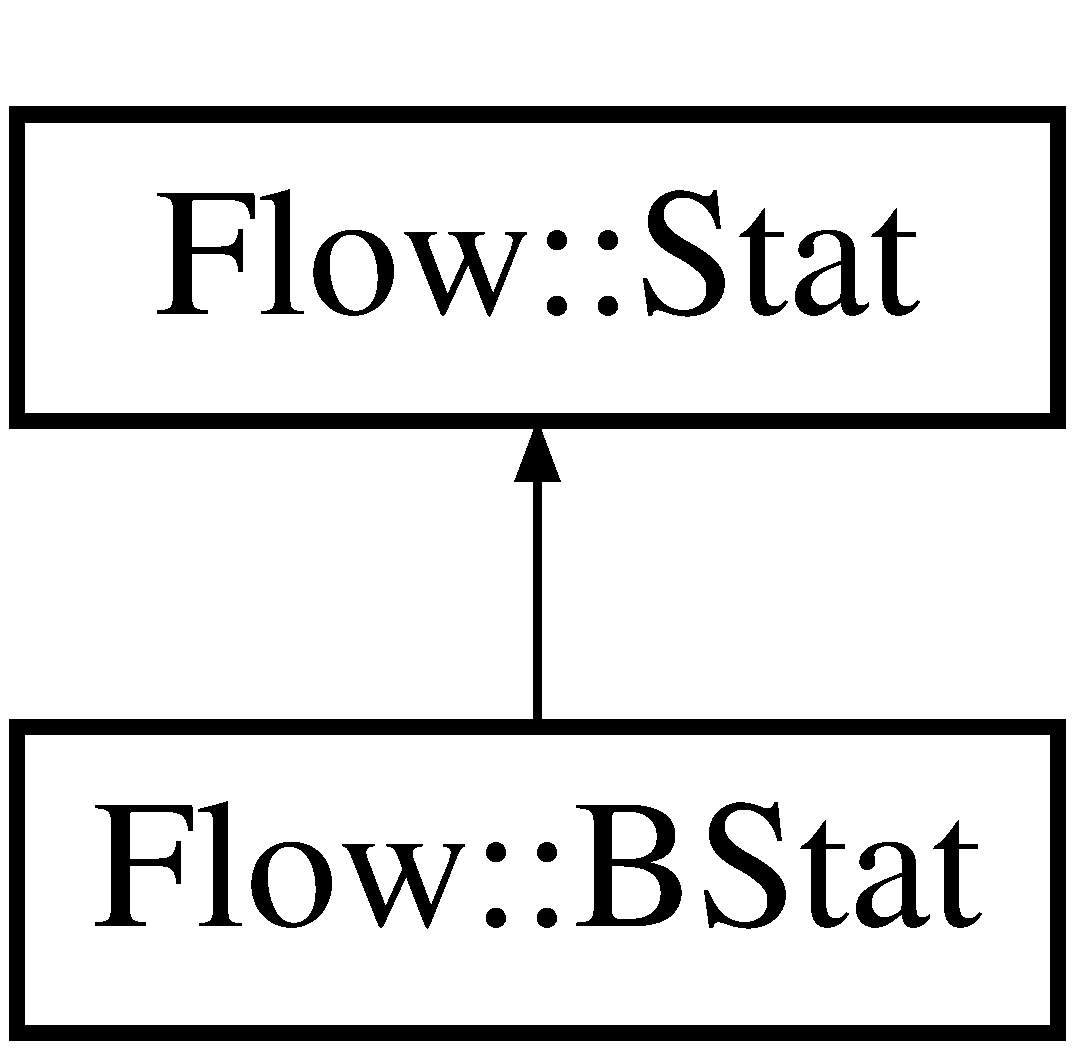
\includegraphics[height=2.000000cm]{class_flow_1_1_b_stat}
\end{center}
\end{figure}
\subsection*{Public Member Functions}
\begin{DoxyCompactItemize}
\item 
\hyperlink{class_flow_1_1_b_stat_ab1b39226cb1935d921c3b3c426f402eb}{B\+Stat} ()
\item 
\hyperlink{class_flow_1_1_b_stat_a757ab02769bb9990f13d9ba2e7f159a0}{B\+Stat} (const std\+::string \&, const std\+::string \&, unsigned char)
\item 
\hyperlink{class_flow_1_1_b_stat_adf5f5a63aa82025e4bd86e0df0c5dfb9}{B\+Stat} (const \hyperlink{class_flow_1_1_b_stat}{B\+Stat} \&)
\item 
void \hyperlink{class_flow_1_1_b_stat_a5613f2ccceaaa1c1b254061b398ec1f0}{set\+Value} (unsigned char)
\item 
unsigned char \hyperlink{class_flow_1_1_b_stat_a38ea6d1d87c1f5fa7951d79bae499e5e}{value} () const
\end{DoxyCompactItemize}


\subsection{Detailed Description}


Definition at line 39 of file Stat.\+h.



\subsection{Constructor \& Destructor Documentation}
\hypertarget{class_flow_1_1_b_stat_ab1b39226cb1935d921c3b3c426f402eb}{}\label{class_flow_1_1_b_stat_ab1b39226cb1935d921c3b3c426f402eb} 
\index{Flow\+::\+B\+Stat@{Flow\+::\+B\+Stat}!B\+Stat@{B\+Stat}}
\index{B\+Stat@{B\+Stat}!Flow\+::\+B\+Stat@{Flow\+::\+B\+Stat}}
\subsubsection{\texorpdfstring{B\+Stat()}{BStat()}\hspace{0.1cm}{\footnotesize\ttfamily [1/3]}}
{\footnotesize\ttfamily Flow\+::\+B\+Stat\+::\+B\+Stat (\begin{DoxyParamCaption}{ }\end{DoxyParamCaption})}



Definition at line 60 of file Stat.\+cpp.

\hypertarget{class_flow_1_1_b_stat_a757ab02769bb9990f13d9ba2e7f159a0}{}\label{class_flow_1_1_b_stat_a757ab02769bb9990f13d9ba2e7f159a0} 
\index{Flow\+::\+B\+Stat@{Flow\+::\+B\+Stat}!B\+Stat@{B\+Stat}}
\index{B\+Stat@{B\+Stat}!Flow\+::\+B\+Stat@{Flow\+::\+B\+Stat}}
\subsubsection{\texorpdfstring{B\+Stat()}{BStat()}\hspace{0.1cm}{\footnotesize\ttfamily [2/3]}}
{\footnotesize\ttfamily Flow\+::\+B\+Stat\+::\+B\+Stat (\begin{DoxyParamCaption}\item[{const std\+::string \&}]{n\+Name,  }\item[{const std\+::string \&}]{n\+Fl\+Name,  }\item[{unsigned char}]{n\+Value }\end{DoxyParamCaption})}



Definition at line 78 of file Stat.\+cpp.

\hypertarget{class_flow_1_1_b_stat_adf5f5a63aa82025e4bd86e0df0c5dfb9}{}\label{class_flow_1_1_b_stat_adf5f5a63aa82025e4bd86e0df0c5dfb9} 
\index{Flow\+::\+B\+Stat@{Flow\+::\+B\+Stat}!B\+Stat@{B\+Stat}}
\index{B\+Stat@{B\+Stat}!Flow\+::\+B\+Stat@{Flow\+::\+B\+Stat}}
\subsubsection{\texorpdfstring{B\+Stat()}{BStat()}\hspace{0.1cm}{\footnotesize\ttfamily [3/3]}}
{\footnotesize\ttfamily Flow\+::\+B\+Stat\+::\+B\+Stat (\begin{DoxyParamCaption}\item[{const \hyperlink{class_flow_1_1_b_stat}{B\+Stat} \&}]{other }\end{DoxyParamCaption})}



Definition at line 69 of file Stat.\+cpp.



\subsection{Member Function Documentation}
\hypertarget{class_flow_1_1_b_stat_a5613f2ccceaaa1c1b254061b398ec1f0}{}\label{class_flow_1_1_b_stat_a5613f2ccceaaa1c1b254061b398ec1f0} 
\index{Flow\+::\+B\+Stat@{Flow\+::\+B\+Stat}!set\+Value@{set\+Value}}
\index{set\+Value@{set\+Value}!Flow\+::\+B\+Stat@{Flow\+::\+B\+Stat}}
\subsubsection{\texorpdfstring{set\+Value()}{setValue()}}
{\footnotesize\ttfamily void Flow\+::\+B\+Stat\+::set\+Value (\begin{DoxyParamCaption}\item[{unsigned char}]{value }\end{DoxyParamCaption})}



Definition at line 99 of file Stat.\+cpp.

\hypertarget{class_flow_1_1_b_stat_a38ea6d1d87c1f5fa7951d79bae499e5e}{}\label{class_flow_1_1_b_stat_a38ea6d1d87c1f5fa7951d79bae499e5e} 
\index{Flow\+::\+B\+Stat@{Flow\+::\+B\+Stat}!value@{value}}
\index{value@{value}!Flow\+::\+B\+Stat@{Flow\+::\+B\+Stat}}
\subsubsection{\texorpdfstring{value()}{value()}}
{\footnotesize\ttfamily unsigned char Flow\+::\+B\+Stat\+::value (\begin{DoxyParamCaption}{ }\end{DoxyParamCaption}) const}



Definition at line 89 of file Stat.\+cpp.



The documentation for this class was generated from the following files\+:\begin{DoxyCompactItemize}
\item 
E\+:/git/gn0mesort/\+Rothman\+Alexander\+\_\+\+C\+S\+C17\+A\+\_\+48096/proj/\+Project\+\_\+1/\+Overflow/\hyperlink{_stat_8h}{Stat.\+h}\item 
E\+:/git/gn0mesort/\+Rothman\+Alexander\+\_\+\+C\+S\+C17\+A\+\_\+48096/proj/\+Project\+\_\+1/\+Overflow/\hyperlink{_stat_8cpp}{Stat.\+cpp}\end{DoxyCompactItemize}

\hypertarget{struct_flow_1_1_config}{}\section{Flow\+:\+:Config Struct Reference}
\label{struct_flow_1_1_config}\index{Flow\+::\+Config@{Flow\+::\+Config}}


{\ttfamily \#include $<$structs.\+h$>$}

\subsection*{Public Attributes}
\begin{DoxyCompactItemize}
\item 
bool \hyperlink{struct_flow_1_1_config_a695298c2ded0f1dc247cd533a98579a1}{ascii\+Art}
\item 
std\+::string \hyperlink{struct_flow_1_1_config_ae9c7f4511035a6c6dbf177435d8835c3}{save\+Game}
\end{DoxyCompactItemize}


\subsection{Detailed Description}
Defines a \hyperlink{class_flow_1_1_game}{Game} configuration 

Definition at line 41 of file structs.\+h.



\subsection{Member Data Documentation}
\hypertarget{struct_flow_1_1_config_a695298c2ded0f1dc247cd533a98579a1}{}\label{struct_flow_1_1_config_a695298c2ded0f1dc247cd533a98579a1} 
\index{Flow\+::\+Config@{Flow\+::\+Config}!ascii\+Art@{ascii\+Art}}
\index{ascii\+Art@{ascii\+Art}!Flow\+::\+Config@{Flow\+::\+Config}}
\subsubsection{\texorpdfstring{ascii\+Art}{asciiArt}}
{\footnotesize\ttfamily bool Flow\+::\+Config\+::ascii\+Art}

Whether or not to display A\+S\+C\+II art 

Definition at line 45 of file structs.\+h.

\hypertarget{struct_flow_1_1_config_ae9c7f4511035a6c6dbf177435d8835c3}{}\label{struct_flow_1_1_config_ae9c7f4511035a6c6dbf177435d8835c3} 
\index{Flow\+::\+Config@{Flow\+::\+Config}!save\+Game@{save\+Game}}
\index{save\+Game@{save\+Game}!Flow\+::\+Config@{Flow\+::\+Config}}
\subsubsection{\texorpdfstring{save\+Game}{saveGame}}
{\footnotesize\ttfamily std\+::string Flow\+::\+Config\+::save\+Game}

The current save path 

Definition at line 50 of file structs.\+h.



The documentation for this struct was generated from the following file\+:\begin{DoxyCompactItemize}
\item 
Rothman\+Alexander\+\_\+\+C\+S\+C17\+A\+\_\+48096/proj/\+Project\+\_\+2/\+Overflow\+\_\+2/\hyperlink{structs_8h}{structs.\+h}\end{DoxyCompactItemize}

\hypertarget{class_flow_1_1_flg_util}{}\section{Flow\+:\+:Flg\+Util Class Reference}
\label{class_flow_1_1_flg_util}\index{Flow\+::\+Flg\+Util@{Flow\+::\+Flg\+Util}}


{\ttfamily \#include $<$Flags.\+h$>$}

\subsection*{Static Public Member Functions}
\begin{DoxyCompactItemize}
\item 
static bool \hyperlink{class_flow_1_1_flg_util_a8e714f79a855912792ea53991ee72c5c}{has\+Flag} (unsigned long data, unsigned long value)
\end{DoxyCompactItemize}


\subsection{Detailed Description}


Definition at line 48 of file Flags.\+h.



\subsection{Member Function Documentation}
\hypertarget{class_flow_1_1_flg_util_a8e714f79a855912792ea53991ee72c5c}{}\label{class_flow_1_1_flg_util_a8e714f79a855912792ea53991ee72c5c} 
\index{Flow\+::\+Flg\+Util@{Flow\+::\+Flg\+Util}!has\+Flag@{has\+Flag}}
\index{has\+Flag@{has\+Flag}!Flow\+::\+Flg\+Util@{Flow\+::\+Flg\+Util}}
\subsubsection{\texorpdfstring{has\+Flag()}{hasFlag()}}
{\footnotesize\ttfamily bool Flow\+::\+Flg\+Util\+::has\+Flag (\begin{DoxyParamCaption}\item[{unsigned long}]{data,  }\item[{unsigned long}]{value }\end{DoxyParamCaption})\hspace{0.3cm}{\ttfamily [static]}}



Definition at line 160 of file Flags.\+cpp.



The documentation for this class was generated from the following files\+:\begin{DoxyCompactItemize}
\item 
E\+:/git/gn0mesort/\+Rothman\+Alexander\+\_\+\+C\+S\+C17\+A\+\_\+48096/proj/\+Project\+\_\+1/\+Overflow/\hyperlink{_flags_8h}{Flags.\+h}\item 
E\+:/git/gn0mesort/\+Rothman\+Alexander\+\_\+\+C\+S\+C17\+A\+\_\+48096/proj/\+Project\+\_\+1/\+Overflow/\hyperlink{_flags_8cpp}{Flags.\+cpp}\end{DoxyCompactItemize}

\hypertarget{class_flow_1_1_floor}{}\section{Flow\+:\+:Floor Class Reference}
\label{class_flow_1_1_floor}\index{Flow\+::\+Floor@{Flow\+::\+Floor}}


{\ttfamily \#include $<$room.\+h$>$}

\subsection*{Public Member Functions}
\begin{DoxyCompactItemize}
\item 
\hyperlink{class_flow_1_1_floor_a056779b11b4084e15cc7c376f791a8f3}{Floor} ()
\item 
\hyperlink{class_flow_1_1_floor_ab4003203c3ad5de4c13d669bddbb0df5}{Floor} (const \hyperlink{class_flow_1_1_floor}{Floor} \&)
\item 
\hyperlink{class_flow_1_1_floor_afc7d87d65bc697a8901ad9506bafb5b9}{Floor} (unsigned char, unsigned char)
\item 
\hyperlink{class_flow_1_1_floor_abcb53e88835e043390289c0aac035ac0}{$\sim$\+Floor} ()
\item 
void \hyperlink{class_flow_1_1_floor_a7fedee1db9c05420cc75bee81c3be0b6}{draw} (const \hyperlink{struct_flow_1_1_point}{Point} \&) const
\item 
void \hyperlink{class_flow_1_1_floor_a9cab7af772e3b3a12f289b0942e870f1}{draw\+Dbg} () const
\item 
bool \hyperlink{class_flow_1_1_floor_a649041679a73f38cf92ef7082c885795}{is\+Overflow} (unsigned char, unsigned char) const
\item 
bool \hyperlink{class_flow_1_1_floor_a6511d441ffd99d0a0d85669cfa846945}{is\+OverflowX} (unsigned char) const
\item 
bool \hyperlink{class_flow_1_1_floor_aae39e73db09b3b26d17dfda7418a67d1}{is\+OverflowY} (unsigned char) const
\item 
bool \hyperlink{class_flow_1_1_floor_a257b06bf103cca41a2b6e42692fb4fbe}{move} (\hyperlink{struct_flow_1_1_point}{Point} \&, unsigned char)
\item 
unsigned char \hyperlink{class_flow_1_1_floor_ad56ae970e75d1be616164efd2f84125b}{sizeX} () const
\item 
unsigned char \hyperlink{class_flow_1_1_floor_a6b25e8faedfd7de16efea8523c45794c}{sizeY} () const
\item 
\hyperlink{struct_flow_1_1_point}{Point} \hyperlink{class_flow_1_1_floor_aaac7f88dd55b4fe38ba36f686109fe7b}{start} () const
\item 
\hyperlink{class_flow_1_1_room}{Room} \hyperlink{class_flow_1_1_floor_a167e37ebab4947cdc191890647ff99e6}{get} (unsigned char, unsigned char) const
\item 
\hyperlink{class_flow_1_1_room}{Room} $\ast$ \hyperlink{class_flow_1_1_floor_a4b76afdb21d1687bd9ed0d37e09a15d7}{operator\mbox{[}$\,$\mbox{]}} (unsigned int)
\item 
\hyperlink{class_flow_1_1_floor}{Floor} \& \hyperlink{class_flow_1_1_floor_a0d053f735a848823fcb7e2f8650090da}{operator=} (const \hyperlink{class_flow_1_1_floor}{Floor} \&)
\end{DoxyCompactItemize}
\subsection*{Static Public Member Functions}
\begin{DoxyCompactItemize}
\item 
static void \hyperlink{class_flow_1_1_floor_a390f2a8e15aa8c4cb50180feda028d5d}{swap} (\hyperlink{class_flow_1_1_floor}{Floor} \&, \hyperlink{class_flow_1_1_floor}{Floor} \&)
\end{DoxyCompactItemize}


\subsection{Detailed Description}
Defines a \hyperlink{class_flow_1_1_floor}{Floor} in the game world. A \hyperlink{class_flow_1_1_floor}{Floor} is a 2D array or Rooms 

Definition at line 70 of file room.\+h.



\subsection{Constructor \& Destructor Documentation}
\hypertarget{class_flow_1_1_floor_a056779b11b4084e15cc7c376f791a8f3}{}\label{class_flow_1_1_floor_a056779b11b4084e15cc7c376f791a8f3} 
\index{Flow\+::\+Floor@{Flow\+::\+Floor}!Floor@{Floor}}
\index{Floor@{Floor}!Flow\+::\+Floor@{Flow\+::\+Floor}}
\subsubsection{\texorpdfstring{Floor()}{Floor()}\hspace{0.1cm}{\footnotesize\ttfamily [1/3]}}
{\footnotesize\ttfamily Flow\+::\+Floor\+::\+Floor (\begin{DoxyParamCaption}{ }\end{DoxyParamCaption})}

Default \hyperlink{class_flow_1_1_floor}{Floor} constructor 

Definition at line 111 of file room.\+cpp.

\hypertarget{class_flow_1_1_floor_ab4003203c3ad5de4c13d669bddbb0df5}{}\label{class_flow_1_1_floor_ab4003203c3ad5de4c13d669bddbb0df5} 
\index{Flow\+::\+Floor@{Flow\+::\+Floor}!Floor@{Floor}}
\index{Floor@{Floor}!Flow\+::\+Floor@{Flow\+::\+Floor}}
\subsubsection{\texorpdfstring{Floor()}{Floor()}\hspace{0.1cm}{\footnotesize\ttfamily [2/3]}}
{\footnotesize\ttfamily Flow\+::\+Floor\+::\+Floor (\begin{DoxyParamCaption}\item[{const \hyperlink{class_flow_1_1_floor}{Floor} \&}]{other }\end{DoxyParamCaption})}

\hyperlink{class_flow_1_1_floor}{Floor} copy constructor 
\begin{DoxyParams}{Parameters}
{\em other} & The \hyperlink{class_flow_1_1_floor}{Floor} to copy from \\
\hline
\end{DoxyParams}


Definition at line 126 of file room.\+cpp.

\hypertarget{class_flow_1_1_floor_afc7d87d65bc697a8901ad9506bafb5b9}{}\label{class_flow_1_1_floor_afc7d87d65bc697a8901ad9506bafb5b9} 
\index{Flow\+::\+Floor@{Flow\+::\+Floor}!Floor@{Floor}}
\index{Floor@{Floor}!Flow\+::\+Floor@{Flow\+::\+Floor}}
\subsubsection{\texorpdfstring{Floor()}{Floor()}\hspace{0.1cm}{\footnotesize\ttfamily [3/3]}}
{\footnotesize\ttfamily Flow\+::\+Floor\+::\+Floor (\begin{DoxyParamCaption}\item[{unsigned char}]{sizeX,  }\item[{unsigned char}]{sizeY }\end{DoxyParamCaption})}

Parameterized \hyperlink{class_flow_1_1_floor}{Floor} constructor 
\begin{DoxyParams}{Parameters}
{\em sizeX} & The X-\/axis size of the \hyperlink{class_flow_1_1_floor}{Floor} \\
\hline
{\em sizeY} & The Y-\/axis size of the \hyperlink{class_flow_1_1_floor}{Floor} \\
\hline
\end{DoxyParams}


Definition at line 145 of file room.\+cpp.

\hypertarget{class_flow_1_1_floor_abcb53e88835e043390289c0aac035ac0}{}\label{class_flow_1_1_floor_abcb53e88835e043390289c0aac035ac0} 
\index{Flow\+::\+Floor@{Flow\+::\+Floor}!````~Floor@{$\sim$\+Floor}}
\index{````~Floor@{$\sim$\+Floor}!Flow\+::\+Floor@{Flow\+::\+Floor}}
\subsubsection{\texorpdfstring{$\sim$\+Floor()}{~Floor()}}
{\footnotesize\ttfamily Flow\+::\+Floor\+::$\sim$\+Floor (\begin{DoxyParamCaption}{ }\end{DoxyParamCaption})}

\hyperlink{class_flow_1_1_floor}{Floor} destructor 

Definition at line 157 of file room.\+cpp.



\subsection{Member Function Documentation}
\hypertarget{class_flow_1_1_floor_a7fedee1db9c05420cc75bee81c3be0b6}{}\label{class_flow_1_1_floor_a7fedee1db9c05420cc75bee81c3be0b6} 
\index{Flow\+::\+Floor@{Flow\+::\+Floor}!draw@{draw}}
\index{draw@{draw}!Flow\+::\+Floor@{Flow\+::\+Floor}}
\subsubsection{\texorpdfstring{draw()}{draw()}}
{\footnotesize\ttfamily void Flow\+::\+Floor\+::draw (\begin{DoxyParamCaption}\item[{const \hyperlink{struct_flow_1_1_point}{Point} \&}]{pos }\end{DoxyParamCaption}) const}

Draw a map of the \hyperlink{class_flow_1_1_floor}{Floor} 
\begin{DoxyParams}{Parameters}
{\em pos} & The position of the \hyperlink{class_flow_1_1_game}{Game}\textquotesingle{}s player \\
\hline
\end{DoxyParams}


Definition at line 196 of file room.\+cpp.

\hypertarget{class_flow_1_1_floor_a9cab7af772e3b3a12f289b0942e870f1}{}\label{class_flow_1_1_floor_a9cab7af772e3b3a12f289b0942e870f1} 
\index{Flow\+::\+Floor@{Flow\+::\+Floor}!draw\+Dbg@{draw\+Dbg}}
\index{draw\+Dbg@{draw\+Dbg}!Flow\+::\+Floor@{Flow\+::\+Floor}}
\subsubsection{\texorpdfstring{draw\+Dbg()}{drawDbg()}}
{\footnotesize\ttfamily void Flow\+::\+Floor\+::draw\+Dbg (\begin{DoxyParamCaption}{ }\end{DoxyParamCaption}) const}

Draw Debug map of the \hyperlink{class_flow_1_1_floor}{Floor} 

Definition at line 221 of file room.\+cpp.

\hypertarget{class_flow_1_1_floor_a167e37ebab4947cdc191890647ff99e6}{}\label{class_flow_1_1_floor_a167e37ebab4947cdc191890647ff99e6} 
\index{Flow\+::\+Floor@{Flow\+::\+Floor}!get@{get}}
\index{get@{get}!Flow\+::\+Floor@{Flow\+::\+Floor}}
\subsubsection{\texorpdfstring{get()}{get()}}
{\footnotesize\ttfamily \hyperlink{class_flow_1_1_room}{Flow\+::\+Room} Flow\+::\+Floor\+::get (\begin{DoxyParamCaption}\item[{unsigned char}]{x,  }\item[{unsigned char}]{y }\end{DoxyParamCaption}) const}

Get a \hyperlink{class_flow_1_1_room}{Room} from the \hyperlink{class_flow_1_1_floor}{Floor} 
\begin{DoxyParams}{Parameters}
{\em x} & The X position of the \hyperlink{class_flow_1_1_room}{Room} \\
\hline
{\em y} & The Y position of the \hyperlink{class_flow_1_1_room}{Room} \\
\hline
\end{DoxyParams}
\begin{DoxyReturn}{Returns}
The \hyperlink{class_flow_1_1_room}{Room} at the given position 
\end{DoxyReturn}


Definition at line 311 of file room.\+cpp.

\hypertarget{class_flow_1_1_floor_a649041679a73f38cf92ef7082c885795}{}\label{class_flow_1_1_floor_a649041679a73f38cf92ef7082c885795} 
\index{Flow\+::\+Floor@{Flow\+::\+Floor}!is\+Overflow@{is\+Overflow}}
\index{is\+Overflow@{is\+Overflow}!Flow\+::\+Floor@{Flow\+::\+Floor}}
\subsubsection{\texorpdfstring{is\+Overflow()}{isOverflow()}}
{\footnotesize\ttfamily bool Flow\+::\+Floor\+::is\+Overflow (\begin{DoxyParamCaption}\item[{unsigned char}]{x,  }\item[{unsigned char}]{y }\end{DoxyParamCaption}) const}

Check whether an (X, Y) position is outside the bounds of the \hyperlink{class_flow_1_1_floor}{Floor} 
\begin{DoxyParams}{Parameters}
{\em x} & The X position \\
\hline
{\em y} & The Y position \\
\hline
\end{DoxyParams}
\begin{DoxyReturn}{Returns}
true if the point is outside the bounds of the \hyperlink{class_flow_1_1_floor}{Floor}. Otherwise false 
\end{DoxyReturn}


Definition at line 239 of file room.\+cpp.

\hypertarget{class_flow_1_1_floor_a6511d441ffd99d0a0d85669cfa846945}{}\label{class_flow_1_1_floor_a6511d441ffd99d0a0d85669cfa846945} 
\index{Flow\+::\+Floor@{Flow\+::\+Floor}!is\+OverflowX@{is\+OverflowX}}
\index{is\+OverflowX@{is\+OverflowX}!Flow\+::\+Floor@{Flow\+::\+Floor}}
\subsubsection{\texorpdfstring{is\+Overflow\+X()}{isOverflowX()}}
{\footnotesize\ttfamily bool Flow\+::\+Floor\+::is\+OverflowX (\begin{DoxyParamCaption}\item[{unsigned char}]{x }\end{DoxyParamCaption}) const}

Check whether an X position is outside the bounds of the \hyperlink{class_flow_1_1_floor}{Floor} 
\begin{DoxyParams}{Parameters}
{\em x} & The X position to check \\
\hline
\end{DoxyParams}
\begin{DoxyReturn}{Returns}
true if the position is outside the bounds of the \hyperlink{class_flow_1_1_floor}{Floor}. Otherwise false 
\end{DoxyReturn}
If greater than sizeX or less than 0 

Definition at line 251 of file room.\+cpp.

\hypertarget{class_flow_1_1_floor_aae39e73db09b3b26d17dfda7418a67d1}{}\label{class_flow_1_1_floor_aae39e73db09b3b26d17dfda7418a67d1} 
\index{Flow\+::\+Floor@{Flow\+::\+Floor}!is\+OverflowY@{is\+OverflowY}}
\index{is\+OverflowY@{is\+OverflowY}!Flow\+::\+Floor@{Flow\+::\+Floor}}
\subsubsection{\texorpdfstring{is\+Overflow\+Y()}{isOverflowY()}}
{\footnotesize\ttfamily bool Flow\+::\+Floor\+::is\+OverflowY (\begin{DoxyParamCaption}\item[{unsigned char}]{y }\end{DoxyParamCaption}) const}

Check whether an Y position is outside the bounds of the \hyperlink{class_flow_1_1_floor}{Floor} 
\begin{DoxyParams}{Parameters}
{\em y} & The Y position to check \\
\hline
\end{DoxyParams}
\begin{DoxyReturn}{Returns}
true if the position is outside the bounds of the \hyperlink{class_flow_1_1_floor}{Floor}. Otherwise false 
\end{DoxyReturn}


Definition at line 263 of file room.\+cpp.

\hypertarget{class_flow_1_1_floor_a257b06bf103cca41a2b6e42692fb4fbe}{}\label{class_flow_1_1_floor_a257b06bf103cca41a2b6e42692fb4fbe} 
\index{Flow\+::\+Floor@{Flow\+::\+Floor}!move@{move}}
\index{move@{move}!Flow\+::\+Floor@{Flow\+::\+Floor}}
\subsubsection{\texorpdfstring{move()}{move()}}
{\footnotesize\ttfamily bool Flow\+::\+Floor\+::move (\begin{DoxyParamCaption}\item[{\hyperlink{struct_flow_1_1_point}{Point} \&}]{pos,  }\item[{unsigned char}]{direct }\end{DoxyParamCaption})}

Move a point within the bounds of a \hyperlink{class_flow_1_1_floor}{Floor} 
\begin{DoxyParams}{Parameters}
{\em pos} & The point to move \\
\hline
{\em direct} & The direction to move in \\
\hline
\end{DoxyParams}
\begin{DoxyReturn}{Returns}
Whether or not the move succeeded 
\end{DoxyReturn}


Definition at line 172 of file room.\+cpp.

\hypertarget{class_flow_1_1_floor_a0d053f735a848823fcb7e2f8650090da}{}\label{class_flow_1_1_floor_a0d053f735a848823fcb7e2f8650090da} 
\index{Flow\+::\+Floor@{Flow\+::\+Floor}!operator=@{operator=}}
\index{operator=@{operator=}!Flow\+::\+Floor@{Flow\+::\+Floor}}
\subsubsection{\texorpdfstring{operator=()}{operator=()}}
{\footnotesize\ttfamily \hyperlink{class_flow_1_1_floor}{Flow\+::\+Floor} \& Flow\+::\+Floor\+::operator= (\begin{DoxyParamCaption}\item[{const \hyperlink{class_flow_1_1_floor}{Floor} \&}]{rhs }\end{DoxyParamCaption})}

\hyperlink{class_flow_1_1_floor}{Floor} assignment operator 
\begin{DoxyParams}{Parameters}
{\em rhs} & The right hand side of the operator \\
\hline
\end{DoxyParams}
\begin{DoxyReturn}{Returns}
A reference to this \hyperlink{class_flow_1_1_floor}{Floor} after assignment 
\end{DoxyReturn}


Definition at line 329 of file room.\+cpp.

\hypertarget{class_flow_1_1_floor_a4b76afdb21d1687bd9ed0d37e09a15d7}{}\label{class_flow_1_1_floor_a4b76afdb21d1687bd9ed0d37e09a15d7} 
\index{Flow\+::\+Floor@{Flow\+::\+Floor}!operator\mbox{[}\mbox{]}@{operator[]}}
\index{operator\mbox{[}\mbox{]}@{operator[]}!Flow\+::\+Floor@{Flow\+::\+Floor}}
\subsubsection{\texorpdfstring{operator[]()}{operator[]()}}
{\footnotesize\ttfamily \hyperlink{class_flow_1_1_room}{Flow\+::\+Room} $\ast$ Flow\+::\+Floor\+::operator\mbox{[}$\,$\mbox{]} (\begin{DoxyParamCaption}\item[{unsigned int}]{index }\end{DoxyParamCaption})}

Get an array of Rooms from the \hyperlink{class_flow_1_1_floor}{Floor} 
\begin{DoxyParams}{Parameters}
{\em index} & The index of the array to get \\
\hline
\end{DoxyParams}
\begin{DoxyReturn}{Returns}
An array of Rooms as a pointer 
\end{DoxyReturn}


Definition at line 320 of file room.\+cpp.

\hypertarget{class_flow_1_1_floor_ad56ae970e75d1be616164efd2f84125b}{}\label{class_flow_1_1_floor_ad56ae970e75d1be616164efd2f84125b} 
\index{Flow\+::\+Floor@{Flow\+::\+Floor}!sizeX@{sizeX}}
\index{sizeX@{sizeX}!Flow\+::\+Floor@{Flow\+::\+Floor}}
\subsubsection{\texorpdfstring{size\+X()}{sizeX()}}
{\footnotesize\ttfamily unsigned char Flow\+::\+Floor\+::sizeX (\begin{DoxyParamCaption}{ }\end{DoxyParamCaption}) const}

Get the X-\/axis size of the \hyperlink{class_flow_1_1_floor}{Floor} \begin{DoxyReturn}{Returns}
The X-\/axis size of the \hyperlink{class_flow_1_1_floor}{Floor} 
\end{DoxyReturn}


Definition at line 274 of file room.\+cpp.

\hypertarget{class_flow_1_1_floor_a6b25e8faedfd7de16efea8523c45794c}{}\label{class_flow_1_1_floor_a6b25e8faedfd7de16efea8523c45794c} 
\index{Flow\+::\+Floor@{Flow\+::\+Floor}!sizeY@{sizeY}}
\index{sizeY@{sizeY}!Flow\+::\+Floor@{Flow\+::\+Floor}}
\subsubsection{\texorpdfstring{size\+Y()}{sizeY()}}
{\footnotesize\ttfamily unsigned char Flow\+::\+Floor\+::sizeY (\begin{DoxyParamCaption}{ }\end{DoxyParamCaption}) const}

Get the Y-\/axis size of the \hyperlink{class_flow_1_1_floor}{Floor} \begin{DoxyReturn}{Returns}
The Y-\/axis size of the \hyperlink{class_flow_1_1_floor}{Floor} 
\end{DoxyReturn}


Definition at line 282 of file room.\+cpp.

\hypertarget{class_flow_1_1_floor_aaac7f88dd55b4fe38ba36f686109fe7b}{}\label{class_flow_1_1_floor_aaac7f88dd55b4fe38ba36f686109fe7b} 
\index{Flow\+::\+Floor@{Flow\+::\+Floor}!start@{start}}
\index{start@{start}!Flow\+::\+Floor@{Flow\+::\+Floor}}
\subsubsection{\texorpdfstring{start()}{start()}}
{\footnotesize\ttfamily \hyperlink{struct_flow_1_1_point}{Flow\+::\+Point} Flow\+::\+Floor\+::start (\begin{DoxyParamCaption}{ }\end{DoxyParamCaption}) const}

Get the starting position for the \hyperlink{class_flow_1_1_floor}{Floor} \begin{DoxyReturn}{Returns}
A \hyperlink{struct_flow_1_1_point}{Point} containing the starting position 
\end{DoxyReturn}


Definition at line 290 of file room.\+cpp.

\hypertarget{class_flow_1_1_floor_a390f2a8e15aa8c4cb50180feda028d5d}{}\label{class_flow_1_1_floor_a390f2a8e15aa8c4cb50180feda028d5d} 
\index{Flow\+::\+Floor@{Flow\+::\+Floor}!swap@{swap}}
\index{swap@{swap}!Flow\+::\+Floor@{Flow\+::\+Floor}}
\subsubsection{\texorpdfstring{swap()}{swap()}}
{\footnotesize\ttfamily void Flow\+::\+Floor\+::swap (\begin{DoxyParamCaption}\item[{\hyperlink{class_flow_1_1_floor}{Floor} \&}]{a,  }\item[{\hyperlink{class_flow_1_1_floor}{Floor} \&}]{b }\end{DoxyParamCaption})\hspace{0.3cm}{\ttfamily [static]}}

Swap 2 Floors 
\begin{DoxyParams}{Parameters}
{\em a} & The first \hyperlink{class_flow_1_1_floor}{Floor} \\
\hline
{\em b} & The second \hyperlink{class_flow_1_1_floor}{Floor} \\
\hline
\end{DoxyParams}


Definition at line 341 of file room.\+cpp.



The documentation for this class was generated from the following files\+:\begin{DoxyCompactItemize}
\item 
Rothman\+Alexander\+\_\+\+C\+S\+C17\+A\+\_\+48096/proj/\+Project\+\_\+2/\+Overflow\+\_\+2/\hyperlink{room_8h}{room.\+h}\item 
Rothman\+Alexander\+\_\+\+C\+S\+C17\+A\+\_\+48096/proj/\+Project\+\_\+2/\+Overflow\+\_\+2/\hyperlink{room_8cpp}{room.\+cpp}\end{DoxyCompactItemize}

\hypertarget{struct_flow_1_1_game}{}\section{Flow\+:\+:Game Struct Reference}
\label{struct_flow_1_1_game}\index{Flow\+::\+Game@{Flow\+::\+Game}}


{\ttfamily \#include $<$Game.\+h$>$}

\subsection*{Static Public Attributes}
\begin{DoxyCompactItemize}
\item 
static const unsigned int \hyperlink{struct_flow_1_1_game_a25fd62c3ab045d2c4e94920359a83a88}{H\+E\+A\+D\+ER} = 0x776f6c66
\item 
static bool \hyperlink{struct_flow_1_1_game_afcbe054fdbcd4eeefabd75ce3ffbe9dd}{over} = false
\item 
static char \hyperlink{struct_flow_1_1_game_a4438db527125bb587f7d2a55ea0c4cec}{input} = 0
\item 
static \hyperlink{struct_flow_1_1_point}{Point} \hyperlink{struct_flow_1_1_game_ac624f04e5b1f64bcc126455cebd657a0}{pos}
\item 
static \hyperlink{struct_flow_1_1_config}{Config} \hyperlink{struct_flow_1_1_game_a1a4562b85733e7edeca321043e08a4a1}{conf}
\item 
static \hyperlink{class_flow_1_1_gm_rand}{Gm\+Rand} \hyperlink{struct_flow_1_1_game_a2472db93858dc5cd513379328fe1bf5b}{gm\+Rand}
\item 
static \hyperlink{class_flow_1_1_actor}{Actor} \hyperlink{struct_flow_1_1_game_a82056349f2d164e104b496d0adf59e61}{player}
\item 
static std\+::vector$<$ std\+::string $>$ \hyperlink{struct_flow_1_1_game_a02e4c98f7e94142c26a0d45068abfbf3}{m\+Menu}
\item 
static std\+::vector$<$ std\+::string $>$ \hyperlink{struct_flow_1_1_game_a02a99aab36d412ff3fa39f33d9d8f75c}{n\+Mons}
\item 
static std\+::vector$<$ std\+::string $>$ \hyperlink{struct_flow_1_1_game_ab8ad15809dbf8afe3c2676e8cb0d2aa2}{b\+Menu}
\item 
static std\+::vector$<$ std\+::string $>$ \hyperlink{struct_flow_1_1_game_abf561ad69faaf819c7b2f2cc62dfae5e}{g\+Menu}
\item 
static std\+::vector$<$ std\+::string $>$ \hyperlink{struct_flow_1_1_game_a2d8ee4def710e9846bf636ecfcf6a5da}{d\+Menu}
\item 
static std\+::vector$<$ std\+::string $>$ $\ast$ \hyperlink{struct_flow_1_1_game_a722e065ecf907576f0b569a242464861}{n\+Items} = N\+U\+LL
\item 
static std\+::vector$<$ std\+::string $>$ $\ast$ \hyperlink{struct_flow_1_1_game_ae8f060eae77f91be1be9d54b58e4cb2b}{n\+Weaps} = N\+U\+LL
\item 
static \hyperlink{class_flow_1_1_floor}{Floor} \hyperlink{struct_flow_1_1_game_adcb177a0b639e9a3919ad9360b89c217}{floor}
\end{DoxyCompactItemize}


\subsection{Detailed Description}


Definition at line 73 of file Game.\+h.



\subsection{Member Data Documentation}
\hypertarget{struct_flow_1_1_game_ab8ad15809dbf8afe3c2676e8cb0d2aa2}{}\label{struct_flow_1_1_game_ab8ad15809dbf8afe3c2676e8cb0d2aa2} 
\index{Flow\+::\+Game@{Flow\+::\+Game}!b\+Menu@{b\+Menu}}
\index{b\+Menu@{b\+Menu}!Flow\+::\+Game@{Flow\+::\+Game}}
\subsubsection{\texorpdfstring{b\+Menu}{bMenu}}
{\footnotesize\ttfamily std\+::vector$<$ std\+::string $>$ Flow\+::\+Game\+::b\+Menu\hspace{0.3cm}{\ttfamily [static]}}



Definition at line 85 of file Game.\+h.

\hypertarget{struct_flow_1_1_game_a1a4562b85733e7edeca321043e08a4a1}{}\label{struct_flow_1_1_game_a1a4562b85733e7edeca321043e08a4a1} 
\index{Flow\+::\+Game@{Flow\+::\+Game}!conf@{conf}}
\index{conf@{conf}!Flow\+::\+Game@{Flow\+::\+Game}}
\subsubsection{\texorpdfstring{conf}{conf}}
{\footnotesize\ttfamily \hyperlink{struct_flow_1_1_config}{Flow\+::\+Config} Flow\+::\+Game\+::conf\hspace{0.3cm}{\ttfamily [static]}}



Definition at line 80 of file Game.\+h.

\hypertarget{struct_flow_1_1_game_a2d8ee4def710e9846bf636ecfcf6a5da}{}\label{struct_flow_1_1_game_a2d8ee4def710e9846bf636ecfcf6a5da} 
\index{Flow\+::\+Game@{Flow\+::\+Game}!d\+Menu@{d\+Menu}}
\index{d\+Menu@{d\+Menu}!Flow\+::\+Game@{Flow\+::\+Game}}
\subsubsection{\texorpdfstring{d\+Menu}{dMenu}}
{\footnotesize\ttfamily std\+::vector$<$ std\+::string $>$ Flow\+::\+Game\+::d\+Menu\hspace{0.3cm}{\ttfamily [static]}}



Definition at line 87 of file Game.\+h.

\hypertarget{struct_flow_1_1_game_adcb177a0b639e9a3919ad9360b89c217}{}\label{struct_flow_1_1_game_adcb177a0b639e9a3919ad9360b89c217} 
\index{Flow\+::\+Game@{Flow\+::\+Game}!floor@{floor}}
\index{floor@{floor}!Flow\+::\+Game@{Flow\+::\+Game}}
\subsubsection{\texorpdfstring{floor}{floor}}
{\footnotesize\ttfamily \hyperlink{class_flow_1_1_floor}{Flow\+::\+Floor} Flow\+::\+Game\+::floor\hspace{0.3cm}{\ttfamily [static]}}



Definition at line 90 of file Game.\+h.

\hypertarget{struct_flow_1_1_game_abf561ad69faaf819c7b2f2cc62dfae5e}{}\label{struct_flow_1_1_game_abf561ad69faaf819c7b2f2cc62dfae5e} 
\index{Flow\+::\+Game@{Flow\+::\+Game}!g\+Menu@{g\+Menu}}
\index{g\+Menu@{g\+Menu}!Flow\+::\+Game@{Flow\+::\+Game}}
\subsubsection{\texorpdfstring{g\+Menu}{gMenu}}
{\footnotesize\ttfamily std\+::vector$<$ std\+::string $>$ Flow\+::\+Game\+::g\+Menu\hspace{0.3cm}{\ttfamily [static]}}



Definition at line 86 of file Game.\+h.

\hypertarget{struct_flow_1_1_game_a2472db93858dc5cd513379328fe1bf5b}{}\label{struct_flow_1_1_game_a2472db93858dc5cd513379328fe1bf5b} 
\index{Flow\+::\+Game@{Flow\+::\+Game}!gm\+Rand@{gm\+Rand}}
\index{gm\+Rand@{gm\+Rand}!Flow\+::\+Game@{Flow\+::\+Game}}
\subsubsection{\texorpdfstring{gm\+Rand}{gmRand}}
{\footnotesize\ttfamily \hyperlink{class_flow_1_1_gm_rand}{Flow\+::\+Gm\+Rand} Flow\+::\+Game\+::gm\+Rand\hspace{0.3cm}{\ttfamily [static]}}



Definition at line 81 of file Game.\+h.

\hypertarget{struct_flow_1_1_game_a25fd62c3ab045d2c4e94920359a83a88}{}\label{struct_flow_1_1_game_a25fd62c3ab045d2c4e94920359a83a88} 
\index{Flow\+::\+Game@{Flow\+::\+Game}!H\+E\+A\+D\+ER@{H\+E\+A\+D\+ER}}
\index{H\+E\+A\+D\+ER@{H\+E\+A\+D\+ER}!Flow\+::\+Game@{Flow\+::\+Game}}
\subsubsection{\texorpdfstring{H\+E\+A\+D\+ER}{HEADER}}
{\footnotesize\ttfamily const unsigned int Flow\+::\+Game\+::\+H\+E\+A\+D\+ER = 0x776f6c66\hspace{0.3cm}{\ttfamily [static]}}



Definition at line 74 of file Game.\+h.

\hypertarget{struct_flow_1_1_game_a4438db527125bb587f7d2a55ea0c4cec}{}\label{struct_flow_1_1_game_a4438db527125bb587f7d2a55ea0c4cec} 
\index{Flow\+::\+Game@{Flow\+::\+Game}!input@{input}}
\index{input@{input}!Flow\+::\+Game@{Flow\+::\+Game}}
\subsubsection{\texorpdfstring{input}{input}}
{\footnotesize\ttfamily char Flow\+::\+Game\+::input = 0\hspace{0.3cm}{\ttfamily [static]}}



Definition at line 78 of file Game.\+h.

\hypertarget{struct_flow_1_1_game_a02e4c98f7e94142c26a0d45068abfbf3}{}\label{struct_flow_1_1_game_a02e4c98f7e94142c26a0d45068abfbf3} 
\index{Flow\+::\+Game@{Flow\+::\+Game}!m\+Menu@{m\+Menu}}
\index{m\+Menu@{m\+Menu}!Flow\+::\+Game@{Flow\+::\+Game}}
\subsubsection{\texorpdfstring{m\+Menu}{mMenu}}
{\footnotesize\ttfamily std\+::vector$<$ std\+::string $>$ Flow\+::\+Game\+::m\+Menu\hspace{0.3cm}{\ttfamily [static]}}



Definition at line 83 of file Game.\+h.

\hypertarget{struct_flow_1_1_game_a722e065ecf907576f0b569a242464861}{}\label{struct_flow_1_1_game_a722e065ecf907576f0b569a242464861} 
\index{Flow\+::\+Game@{Flow\+::\+Game}!n\+Items@{n\+Items}}
\index{n\+Items@{n\+Items}!Flow\+::\+Game@{Flow\+::\+Game}}
\subsubsection{\texorpdfstring{n\+Items}{nItems}}
{\footnotesize\ttfamily std\+::vector$<$ std\+::string $>$ $\ast$ Flow\+::\+Game\+::n\+Items = N\+U\+LL\hspace{0.3cm}{\ttfamily [static]}}



Definition at line 88 of file Game.\+h.

\hypertarget{struct_flow_1_1_game_a02a99aab36d412ff3fa39f33d9d8f75c}{}\label{struct_flow_1_1_game_a02a99aab36d412ff3fa39f33d9d8f75c} 
\index{Flow\+::\+Game@{Flow\+::\+Game}!n\+Mons@{n\+Mons}}
\index{n\+Mons@{n\+Mons}!Flow\+::\+Game@{Flow\+::\+Game}}
\subsubsection{\texorpdfstring{n\+Mons}{nMons}}
{\footnotesize\ttfamily std\+::vector$<$ std\+::string $>$ Flow\+::\+Game\+::n\+Mons\hspace{0.3cm}{\ttfamily [static]}}



Definition at line 84 of file Game.\+h.

\hypertarget{struct_flow_1_1_game_ae8f060eae77f91be1be9d54b58e4cb2b}{}\label{struct_flow_1_1_game_ae8f060eae77f91be1be9d54b58e4cb2b} 
\index{Flow\+::\+Game@{Flow\+::\+Game}!n\+Weaps@{n\+Weaps}}
\index{n\+Weaps@{n\+Weaps}!Flow\+::\+Game@{Flow\+::\+Game}}
\subsubsection{\texorpdfstring{n\+Weaps}{nWeaps}}
{\footnotesize\ttfamily std\+::vector$<$ std\+::string $>$ $\ast$ Flow\+::\+Game\+::n\+Weaps = N\+U\+LL\hspace{0.3cm}{\ttfamily [static]}}



Definition at line 89 of file Game.\+h.

\hypertarget{struct_flow_1_1_game_afcbe054fdbcd4eeefabd75ce3ffbe9dd}{}\label{struct_flow_1_1_game_afcbe054fdbcd4eeefabd75ce3ffbe9dd} 
\index{Flow\+::\+Game@{Flow\+::\+Game}!over@{over}}
\index{over@{over}!Flow\+::\+Game@{Flow\+::\+Game}}
\subsubsection{\texorpdfstring{over}{over}}
{\footnotesize\ttfamily bool Flow\+::\+Game\+::over = false\hspace{0.3cm}{\ttfamily [static]}}



Definition at line 77 of file Game.\+h.

\hypertarget{struct_flow_1_1_game_a82056349f2d164e104b496d0adf59e61}{}\label{struct_flow_1_1_game_a82056349f2d164e104b496d0adf59e61} 
\index{Flow\+::\+Game@{Flow\+::\+Game}!player@{player}}
\index{player@{player}!Flow\+::\+Game@{Flow\+::\+Game}}
\subsubsection{\texorpdfstring{player}{player}}
{\footnotesize\ttfamily \hyperlink{class_flow_1_1_actor}{Flow\+::\+Actor} Flow\+::\+Game\+::player\hspace{0.3cm}{\ttfamily [static]}}



Definition at line 82 of file Game.\+h.

\hypertarget{struct_flow_1_1_game_ac624f04e5b1f64bcc126455cebd657a0}{}\label{struct_flow_1_1_game_ac624f04e5b1f64bcc126455cebd657a0} 
\index{Flow\+::\+Game@{Flow\+::\+Game}!pos@{pos}}
\index{pos@{pos}!Flow\+::\+Game@{Flow\+::\+Game}}
\subsubsection{\texorpdfstring{pos}{pos}}
{\footnotesize\ttfamily \hyperlink{struct_flow_1_1_point}{Flow\+::\+Point} Flow\+::\+Game\+::pos\hspace{0.3cm}{\ttfamily [static]}}



Definition at line 79 of file Game.\+h.



The documentation for this struct was generated from the following files\+:\begin{DoxyCompactItemize}
\item 
E\+:/git/gn0mesort/\+Rothman\+Alexander\+\_\+\+C\+S\+C17\+A\+\_\+48096/proj/\+Project\+\_\+1/\+Overflow/\hyperlink{_game_8h}{Game.\+h}\item 
E\+:/git/gn0mesort/\+Rothman\+Alexander\+\_\+\+C\+S\+C17\+A\+\_\+48096/proj/\+Project\+\_\+1/\+Overflow/\hyperlink{_game_8cpp}{Game.\+cpp}\end{DoxyCompactItemize}

\hypertarget{class_flow_1_1_gm_rand}{}\section{Flow\+:\+:Gm\+Rand Class Reference}
\label{class_flow_1_1_gm_rand}\index{Flow\+::\+Gm\+Rand@{Flow\+::\+Gm\+Rand}}


{\ttfamily \#include $<$random.\+h$>$}

\subsection*{Public Member Functions}
\begin{DoxyCompactItemize}
\item 
void \hyperlink{class_flow_1_1_gm_rand_a109fe067556f62419afe48f11048acf5}{seek} (unsigned int)
\item 
void \hyperlink{class_flow_1_1_gm_rand_a75eb20ea46c459b53793960e711dd81c}{seek} (const \hyperlink{struct_flow_1_1_r_n_g_point}{R\+N\+G\+Point} \&)
\item 
void \hyperlink{class_flow_1_1_gm_rand_aadd656b294e8e7330ba408486646e2f3}{srand} ()
\item 
void \hyperlink{class_flow_1_1_gm_rand_abc8aefeb9e15a414964e6e9b0665a8e7}{srand} (unsigned int)
\item 
unsigned char \hyperlink{class_flow_1_1_gm_rand_aeb38e9d08aae7a5d4788facf408b01dc}{r\+Direct} ()
\item 
unsigned char \hyperlink{class_flow_1_1_gm_rand_a7df923fe60c18e20a157de7aa599f533}{r\+Elem} ()
\item 
unsigned int \hyperlink{class_flow_1_1_gm_rand_a8a8b7dafe3991717c68beb1f13409f77}{seed} ()
\item 
unsigned int \hyperlink{class_flow_1_1_gm_rand_aef1a411df95f3d49a7180fbcd9d432c1}{pos} ()
\item 
int \hyperlink{class_flow_1_1_gm_rand_a638c37993080f31a9857d11c284c15b5}{rand} ()
\item 
\hyperlink{class_flow_1_1_room}{Room} \hyperlink{class_flow_1_1_gm_rand_a8a978d8967082e7e519996204c29eb9d}{r\+Room} (bool=false, bool=false)
\item 
\hyperlink{class_flow_1_1_floor}{Floor} \hyperlink{class_flow_1_1_gm_rand_a9ca568e62a941c10e42bedb3e334ed52}{r\+Floor} (unsigned char=32)
\end{DoxyCompactItemize}


\subsection{Detailed Description}
Defines an object which allows access to the \hyperlink{class_flow_1_1_gm_rand_a638c37993080f31a9857d11c284c15b5}{rand()} function and records the number of generations which have occurred 

Definition at line 29 of file random.\+h.



\subsection{Member Function Documentation}
\hypertarget{class_flow_1_1_gm_rand_aef1a411df95f3d49a7180fbcd9d432c1}{}\label{class_flow_1_1_gm_rand_aef1a411df95f3d49a7180fbcd9d432c1} 
\index{Flow\+::\+Gm\+Rand@{Flow\+::\+Gm\+Rand}!pos@{pos}}
\index{pos@{pos}!Flow\+::\+Gm\+Rand@{Flow\+::\+Gm\+Rand}}
\subsubsection{\texorpdfstring{pos()}{pos()}}
{\footnotesize\ttfamily unsigned int Flow\+::\+Gm\+Rand\+::pos (\begin{DoxyParamCaption}{ }\end{DoxyParamCaption})}

Get the position of the R\+NG \begin{DoxyReturn}{Returns}
The position of the R\+NG in calls to \hyperlink{class_flow_1_1_gm_rand_a638c37993080f31a9857d11c284c15b5}{rand()} from 0 
\end{DoxyReturn}


Definition at line 65 of file random.\+cpp.

\hypertarget{class_flow_1_1_gm_rand_a638c37993080f31a9857d11c284c15b5}{}\label{class_flow_1_1_gm_rand_a638c37993080f31a9857d11c284c15b5} 
\index{Flow\+::\+Gm\+Rand@{Flow\+::\+Gm\+Rand}!rand@{rand}}
\index{rand@{rand}!Flow\+::\+Gm\+Rand@{Flow\+::\+Gm\+Rand}}
\subsubsection{\texorpdfstring{rand()}{rand()}}
{\footnotesize\ttfamily int Flow\+::\+Gm\+Rand\+::rand (\begin{DoxyParamCaption}{ }\end{DoxyParamCaption})}

Generate a random number \begin{DoxyReturn}{Returns}
A random int 
\end{DoxyReturn}


Definition at line 44 of file random.\+cpp.

\hypertarget{class_flow_1_1_gm_rand_aeb38e9d08aae7a5d4788facf408b01dc}{}\label{class_flow_1_1_gm_rand_aeb38e9d08aae7a5d4788facf408b01dc} 
\index{Flow\+::\+Gm\+Rand@{Flow\+::\+Gm\+Rand}!r\+Direct@{r\+Direct}}
\index{r\+Direct@{r\+Direct}!Flow\+::\+Gm\+Rand@{Flow\+::\+Gm\+Rand}}
\subsubsection{\texorpdfstring{r\+Direct()}{rDirect()}}
{\footnotesize\ttfamily unsigned char Flow\+::\+Gm\+Rand\+::r\+Direct (\begin{DoxyParamCaption}{ }\end{DoxyParamCaption})}

Generate a random direction. Always cardinal \begin{DoxyReturn}{Returns}
The generated direction 
\end{DoxyReturn}


Definition at line 189 of file random.\+cpp.

\hypertarget{class_flow_1_1_gm_rand_a7df923fe60c18e20a157de7aa599f533}{}\label{class_flow_1_1_gm_rand_a7df923fe60c18e20a157de7aa599f533} 
\index{Flow\+::\+Gm\+Rand@{Flow\+::\+Gm\+Rand}!r\+Elem@{r\+Elem}}
\index{r\+Elem@{r\+Elem}!Flow\+::\+Gm\+Rand@{Flow\+::\+Gm\+Rand}}
\subsubsection{\texorpdfstring{r\+Elem()}{rElem()}}
{\footnotesize\ttfamily unsigned char Flow\+::\+Gm\+Rand\+::r\+Elem (\begin{DoxyParamCaption}{ }\end{DoxyParamCaption})}

Get a random element \begin{DoxyReturn}{Returns}
A random element based on the game\textquotesingle{}s set probabilities 
\end{DoxyReturn}
10\% chance of possible multiple enchants 

Definition at line 81 of file random.\+cpp.

\hypertarget{class_flow_1_1_gm_rand_a9ca568e62a941c10e42bedb3e334ed52}{}\label{class_flow_1_1_gm_rand_a9ca568e62a941c10e42bedb3e334ed52} 
\index{Flow\+::\+Gm\+Rand@{Flow\+::\+Gm\+Rand}!r\+Floor@{r\+Floor}}
\index{r\+Floor@{r\+Floor}!Flow\+::\+Gm\+Rand@{Flow\+::\+Gm\+Rand}}
\subsubsection{\texorpdfstring{r\+Floor()}{rFloor()}}
{\footnotesize\ttfamily \hyperlink{class_flow_1_1_floor}{Flow\+::\+Floor} Flow\+::\+Gm\+Rand\+::r\+Floor (\begin{DoxyParamCaption}\item[{unsigned char}]{size = {\ttfamily 32} }\end{DoxyParamCaption})}

Generate a random \hyperlink{class_flow_1_1_floor}{Floor} 
\begin{DoxyParams}{Parameters}
{\em size} & The size of the \hyperlink{class_flow_1_1_floor}{Floor} to generate \\
\hline
\end{DoxyParams}
\begin{DoxyReturn}{Returns}
The generated \hyperlink{class_flow_1_1_floor}{Floor} object 
\end{DoxyReturn}


Definition at line 112 of file random.\+cpp.

\hypertarget{class_flow_1_1_gm_rand_a8a978d8967082e7e519996204c29eb9d}{}\label{class_flow_1_1_gm_rand_a8a978d8967082e7e519996204c29eb9d} 
\index{Flow\+::\+Gm\+Rand@{Flow\+::\+Gm\+Rand}!r\+Room@{r\+Room}}
\index{r\+Room@{r\+Room}!Flow\+::\+Gm\+Rand@{Flow\+::\+Gm\+Rand}}
\subsubsection{\texorpdfstring{r\+Room()}{rRoom()}}
{\footnotesize\ttfamily \hyperlink{class_flow_1_1_room}{Flow\+::\+Room} Flow\+::\+Gm\+Rand\+::r\+Room (\begin{DoxyParamCaption}\item[{bool}]{start = {\ttfamily false},  }\item[{bool}]{end = {\ttfamily false} }\end{DoxyParamCaption})}

Generate a random \hyperlink{class_flow_1_1_room}{Room} 
\begin{DoxyParams}{Parameters}
{\em start} & Whether or not the \hyperlink{class_flow_1_1_room}{Room} is the starting \hyperlink{class_flow_1_1_room}{Room} \\
\hline
{\em end} & Whether or not the \hyperlink{class_flow_1_1_room}{Room} is the ending \hyperlink{class_flow_1_1_room}{Room} \\
\hline
\end{DoxyParams}
\begin{DoxyReturn}{Returns}
The generated \hyperlink{class_flow_1_1_room}{Room} 
\end{DoxyReturn}


Definition at line 168 of file random.\+cpp.

\hypertarget{class_flow_1_1_gm_rand_a8a8b7dafe3991717c68beb1f13409f77}{}\label{class_flow_1_1_gm_rand_a8a8b7dafe3991717c68beb1f13409f77} 
\index{Flow\+::\+Gm\+Rand@{Flow\+::\+Gm\+Rand}!seed@{seed}}
\index{seed@{seed}!Flow\+::\+Gm\+Rand@{Flow\+::\+Gm\+Rand}}
\subsubsection{\texorpdfstring{seed()}{seed()}}
{\footnotesize\ttfamily unsigned int Flow\+::\+Gm\+Rand\+::seed (\begin{DoxyParamCaption}{ }\end{DoxyParamCaption})}

Get the seed of the R\+NG \begin{DoxyReturn}{Returns}
The current seed value 
\end{DoxyReturn}


Definition at line 73 of file random.\+cpp.

\hypertarget{class_flow_1_1_gm_rand_a109fe067556f62419afe48f11048acf5}{}\label{class_flow_1_1_gm_rand_a109fe067556f62419afe48f11048acf5} 
\index{Flow\+::\+Gm\+Rand@{Flow\+::\+Gm\+Rand}!seek@{seek}}
\index{seek@{seek}!Flow\+::\+Gm\+Rand@{Flow\+::\+Gm\+Rand}}
\subsubsection{\texorpdfstring{seek()}{seek()}\hspace{0.1cm}{\footnotesize\ttfamily [1/2]}}
{\footnotesize\ttfamily void Flow\+::\+Gm\+Rand\+::seek (\begin{DoxyParamCaption}\item[{unsigned int}]{pos }\end{DoxyParamCaption})}

Seek the R\+NG by reseeding it and calling \hyperlink{class_flow_1_1_gm_rand_a638c37993080f31a9857d11c284c15b5}{rand()} 
\begin{DoxyParams}{Parameters}
{\em pos} & The position to seek to \\
\hline
\end{DoxyParams}


Definition at line 53 of file random.\+cpp.

\hypertarget{class_flow_1_1_gm_rand_a75eb20ea46c459b53793960e711dd81c}{}\label{class_flow_1_1_gm_rand_a75eb20ea46c459b53793960e711dd81c} 
\index{Flow\+::\+Gm\+Rand@{Flow\+::\+Gm\+Rand}!seek@{seek}}
\index{seek@{seek}!Flow\+::\+Gm\+Rand@{Flow\+::\+Gm\+Rand}}
\subsubsection{\texorpdfstring{seek()}{seek()}\hspace{0.1cm}{\footnotesize\ttfamily [2/2]}}
{\footnotesize\ttfamily void Flow\+::\+Gm\+Rand\+::seek (\begin{DoxyParamCaption}\item[{const \hyperlink{struct_flow_1_1_r_n_g_point}{R\+N\+G\+Point} \&}]{point }\end{DoxyParamCaption})}

Seek the position of the R\+NG to the a position in an \hyperlink{struct_flow_1_1_r_n_g_point}{R\+N\+G\+Point}. Reseeds the generator 
\begin{DoxyParams}{Parameters}
{\em point} & \\
\hline
\end{DoxyParams}


Definition at line 102 of file random.\+cpp.

\hypertarget{class_flow_1_1_gm_rand_aadd656b294e8e7330ba408486646e2f3}{}\label{class_flow_1_1_gm_rand_aadd656b294e8e7330ba408486646e2f3} 
\index{Flow\+::\+Gm\+Rand@{Flow\+::\+Gm\+Rand}!srand@{srand}}
\index{srand@{srand}!Flow\+::\+Gm\+Rand@{Flow\+::\+Gm\+Rand}}
\subsubsection{\texorpdfstring{srand()}{srand()}\hspace{0.1cm}{\footnotesize\ttfamily [1/2]}}
{\footnotesize\ttfamily void Flow\+::\+Gm\+Rand\+::srand (\begin{DoxyParamCaption}{ }\end{DoxyParamCaption})}

Seed the random number generator with the current time 

Definition at line 22 of file random.\+cpp.

\hypertarget{class_flow_1_1_gm_rand_abc8aefeb9e15a414964e6e9b0665a8e7}{}\label{class_flow_1_1_gm_rand_abc8aefeb9e15a414964e6e9b0665a8e7} 
\index{Flow\+::\+Gm\+Rand@{Flow\+::\+Gm\+Rand}!srand@{srand}}
\index{srand@{srand}!Flow\+::\+Gm\+Rand@{Flow\+::\+Gm\+Rand}}
\subsubsection{\texorpdfstring{srand()}{srand()}\hspace{0.1cm}{\footnotesize\ttfamily [2/2]}}
{\footnotesize\ttfamily void Flow\+::\+Gm\+Rand\+::srand (\begin{DoxyParamCaption}\item[{unsigned int}]{seed }\end{DoxyParamCaption})}

Seed the random number generator with the input seed 
\begin{DoxyParams}{Parameters}
{\em seed} & The seed to use \\
\hline
\end{DoxyParams}


Definition at line 33 of file random.\+cpp.



The documentation for this class was generated from the following files\+:\begin{DoxyCompactItemize}
\item 
Rothman\+Alexander\+\_\+\+C\+S\+C17\+A\+\_\+48096/proj/\+Project\+\_\+2/\+Overflow\+\_\+2/\hyperlink{random_8h}{random.\+h}\item 
Rothman\+Alexander\+\_\+\+C\+S\+C17\+A\+\_\+48096/proj/\+Project\+\_\+2/\+Overflow\+\_\+2/\hyperlink{random_8cpp}{random.\+cpp}\end{DoxyCompactItemize}

\hypertarget{class_flow_1_1_i_stat}{}\section{Flow\+:\+:I\+Stat Class Reference}
\label{class_flow_1_1_i_stat}\index{Flow\+::\+I\+Stat@{Flow\+::\+I\+Stat}}


{\ttfamily \#include $<$Stat.\+h$>$}

Inheritance diagram for Flow\+:\+:I\+Stat\+:\begin{figure}[H]
\begin{center}
\leavevmode
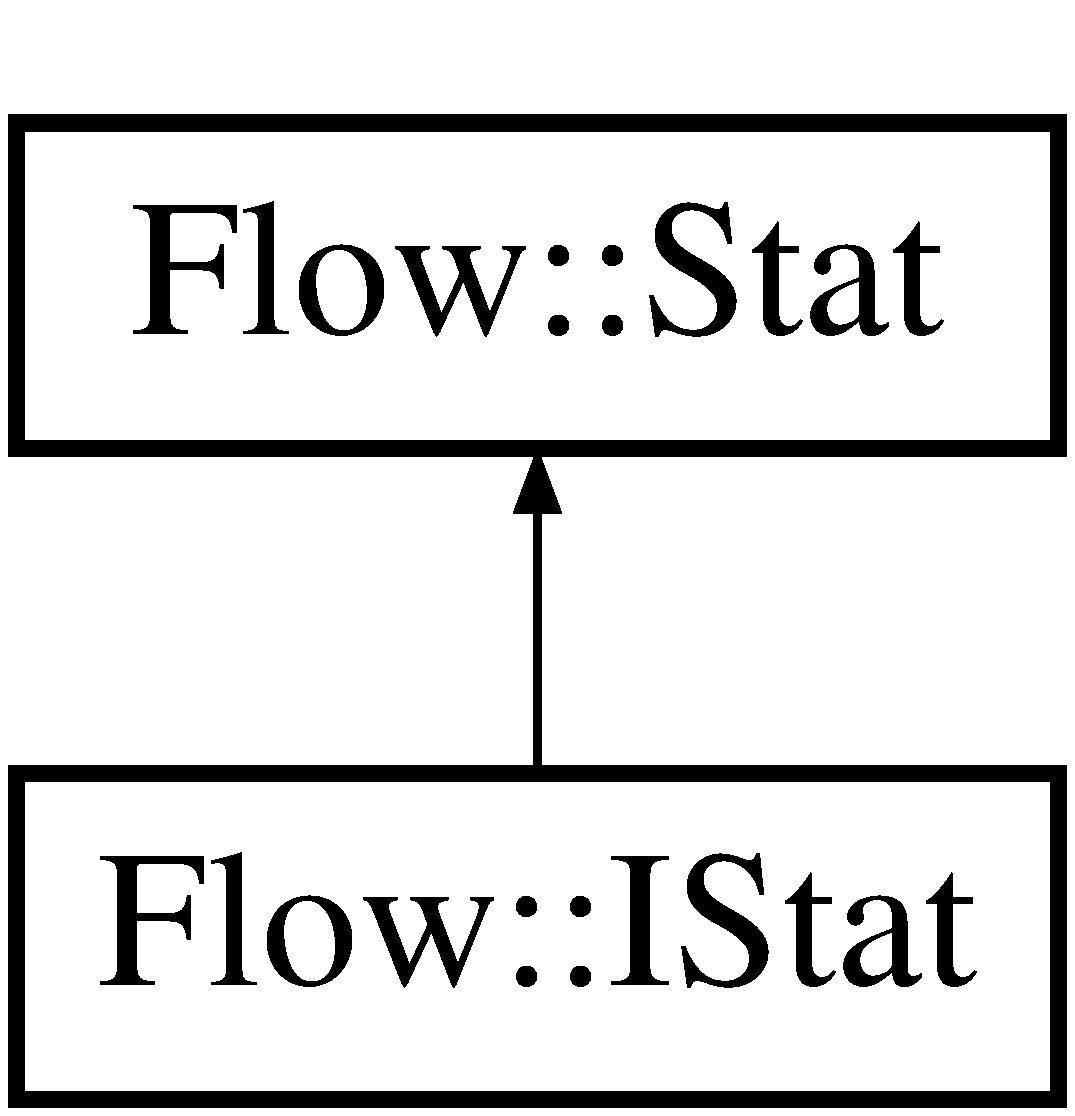
\includegraphics[height=2.000000cm]{class_flow_1_1_i_stat}
\end{center}
\end{figure}
\subsection*{Public Member Functions}
\begin{DoxyCompactItemize}
\item 
\hyperlink{class_flow_1_1_i_stat_ae9fdfde363f2c72f49cc12e6675b143d}{I\+Stat} ()
\item 
\hyperlink{class_flow_1_1_i_stat_ad1dbf438931a51b7f9c3435f63a782fd}{I\+Stat} (const \hyperlink{class_flow_1_1_i_stat}{I\+Stat} \&)
\item 
\hyperlink{class_flow_1_1_i_stat_a1511765ad0b6de79922c5edeff297960}{I\+Stat} (const std\+::string \&\hyperlink{class_flow_1_1_stat_a3b09172b24c2ea0b6a040861b13ac16a}{name}, const std\+::string \&\hyperlink{class_flow_1_1_stat_a82e355b6052a2bc3433dc1f8e48204fc}{fl\+Name}, int \hyperlink{class_flow_1_1_i_stat_aba43e05c007843c7085a6966842e305c}{value}, int \hyperlink{class_flow_1_1_i_stat_abe1547a7dd83b47c0f60ad7aedaa1116}{max}=100, int \hyperlink{class_flow_1_1_i_stat_aae6da9e74e17f356697e518ba3974f70}{min}=0, int \hyperlink{class_flow_1_1_i_stat_a4dcf3ab54ecddbdae7ccdfb86178109f}{abs\+Max}=9999, int \hyperlink{class_flow_1_1_i_stat_a19c20be8f2389371480f2cd07066d387}{abs\+Min}=0)
\item 
void \hyperlink{class_flow_1_1_i_stat_aca87e5a3e7de304739f9a32d5176b0ee}{set\+Max} (int)
\item 
void \hyperlink{class_flow_1_1_i_stat_a63acbda4a0cf88f55401e11fd79b4500}{set\+Min} (int)
\item 
void \hyperlink{class_flow_1_1_i_stat_a96644e89411ca827923e153693a2b9be}{set\+Value} (int)
\item 
int \hyperlink{class_flow_1_1_i_stat_a4dcf3ab54ecddbdae7ccdfb86178109f}{abs\+Max} () const
\item 
int \hyperlink{class_flow_1_1_i_stat_a19c20be8f2389371480f2cd07066d387}{abs\+Min} () const
\item 
int \hyperlink{class_flow_1_1_i_stat_abe1547a7dd83b47c0f60ad7aedaa1116}{max} () const
\item 
int \hyperlink{class_flow_1_1_i_stat_aae6da9e74e17f356697e518ba3974f70}{min} () const
\item 
int \hyperlink{class_flow_1_1_i_stat_aba43e05c007843c7085a6966842e305c}{value} () const
\end{DoxyCompactItemize}


\subsection{Detailed Description}


Definition at line 54 of file Stat.\+h.



\subsection{Constructor \& Destructor Documentation}
\hypertarget{class_flow_1_1_i_stat_ae9fdfde363f2c72f49cc12e6675b143d}{}\label{class_flow_1_1_i_stat_ae9fdfde363f2c72f49cc12e6675b143d} 
\index{Flow\+::\+I\+Stat@{Flow\+::\+I\+Stat}!I\+Stat@{I\+Stat}}
\index{I\+Stat@{I\+Stat}!Flow\+::\+I\+Stat@{Flow\+::\+I\+Stat}}
\subsubsection{\texorpdfstring{I\+Stat()}{IStat()}\hspace{0.1cm}{\footnotesize\ttfamily [1/3]}}
{\footnotesize\ttfamily Flow\+::\+I\+Stat\+::\+I\+Stat (\begin{DoxyParamCaption}{ }\end{DoxyParamCaption})}



Definition at line 106 of file Stat.\+cpp.

\hypertarget{class_flow_1_1_i_stat_ad1dbf438931a51b7f9c3435f63a782fd}{}\label{class_flow_1_1_i_stat_ad1dbf438931a51b7f9c3435f63a782fd} 
\index{Flow\+::\+I\+Stat@{Flow\+::\+I\+Stat}!I\+Stat@{I\+Stat}}
\index{I\+Stat@{I\+Stat}!Flow\+::\+I\+Stat@{Flow\+::\+I\+Stat}}
\subsubsection{\texorpdfstring{I\+Stat()}{IStat()}\hspace{0.1cm}{\footnotesize\ttfamily [2/3]}}
{\footnotesize\ttfamily Flow\+::\+I\+Stat\+::\+I\+Stat (\begin{DoxyParamCaption}\item[{const \hyperlink{class_flow_1_1_i_stat}{I\+Stat} \&}]{other }\end{DoxyParamCaption})}



Definition at line 119 of file Stat.\+cpp.

\hypertarget{class_flow_1_1_i_stat_a1511765ad0b6de79922c5edeff297960}{}\label{class_flow_1_1_i_stat_a1511765ad0b6de79922c5edeff297960} 
\index{Flow\+::\+I\+Stat@{Flow\+::\+I\+Stat}!I\+Stat@{I\+Stat}}
\index{I\+Stat@{I\+Stat}!Flow\+::\+I\+Stat@{Flow\+::\+I\+Stat}}
\subsubsection{\texorpdfstring{I\+Stat()}{IStat()}\hspace{0.1cm}{\footnotesize\ttfamily [3/3]}}
{\footnotesize\ttfamily Flow\+::\+I\+Stat\+::\+I\+Stat (\begin{DoxyParamCaption}\item[{const std\+::string \&}]{name,  }\item[{const std\+::string \&}]{fl\+Name,  }\item[{int}]{value,  }\item[{int}]{max = {\ttfamily 100},  }\item[{int}]{min = {\ttfamily 0},  }\item[{int}]{abs\+Max = {\ttfamily 9999},  }\item[{int}]{abs\+Min = {\ttfamily 0} }\end{DoxyParamCaption})}



Definition at line 133 of file Stat.\+cpp.



\subsection{Member Function Documentation}
\hypertarget{class_flow_1_1_i_stat_a4dcf3ab54ecddbdae7ccdfb86178109f}{}\label{class_flow_1_1_i_stat_a4dcf3ab54ecddbdae7ccdfb86178109f} 
\index{Flow\+::\+I\+Stat@{Flow\+::\+I\+Stat}!abs\+Max@{abs\+Max}}
\index{abs\+Max@{abs\+Max}!Flow\+::\+I\+Stat@{Flow\+::\+I\+Stat}}
\subsubsection{\texorpdfstring{abs\+Max()}{absMax()}}
{\footnotesize\ttfamily int Flow\+::\+I\+Stat\+::abs\+Max (\begin{DoxyParamCaption}{ }\end{DoxyParamCaption}) const}



Definition at line 157 of file Stat.\+cpp.

\hypertarget{class_flow_1_1_i_stat_a19c20be8f2389371480f2cd07066d387}{}\label{class_flow_1_1_i_stat_a19c20be8f2389371480f2cd07066d387} 
\index{Flow\+::\+I\+Stat@{Flow\+::\+I\+Stat}!abs\+Min@{abs\+Min}}
\index{abs\+Min@{abs\+Min}!Flow\+::\+I\+Stat@{Flow\+::\+I\+Stat}}
\subsubsection{\texorpdfstring{abs\+Min()}{absMin()}}
{\footnotesize\ttfamily int Flow\+::\+I\+Stat\+::abs\+Min (\begin{DoxyParamCaption}{ }\end{DoxyParamCaption}) const}



Definition at line 166 of file Stat.\+cpp.

\hypertarget{class_flow_1_1_i_stat_abe1547a7dd83b47c0f60ad7aedaa1116}{}\label{class_flow_1_1_i_stat_abe1547a7dd83b47c0f60ad7aedaa1116} 
\index{Flow\+::\+I\+Stat@{Flow\+::\+I\+Stat}!max@{max}}
\index{max@{max}!Flow\+::\+I\+Stat@{Flow\+::\+I\+Stat}}
\subsubsection{\texorpdfstring{max()}{max()}}
{\footnotesize\ttfamily int Flow\+::\+I\+Stat\+::max (\begin{DoxyParamCaption}{ }\end{DoxyParamCaption}) const}



Definition at line 175 of file Stat.\+cpp.

\hypertarget{class_flow_1_1_i_stat_aae6da9e74e17f356697e518ba3974f70}{}\label{class_flow_1_1_i_stat_aae6da9e74e17f356697e518ba3974f70} 
\index{Flow\+::\+I\+Stat@{Flow\+::\+I\+Stat}!min@{min}}
\index{min@{min}!Flow\+::\+I\+Stat@{Flow\+::\+I\+Stat}}
\subsubsection{\texorpdfstring{min()}{min()}}
{\footnotesize\ttfamily int Flow\+::\+I\+Stat\+::min (\begin{DoxyParamCaption}{ }\end{DoxyParamCaption}) const}



Definition at line 184 of file Stat.\+cpp.

\hypertarget{class_flow_1_1_i_stat_aca87e5a3e7de304739f9a32d5176b0ee}{}\label{class_flow_1_1_i_stat_aca87e5a3e7de304739f9a32d5176b0ee} 
\index{Flow\+::\+I\+Stat@{Flow\+::\+I\+Stat}!set\+Max@{set\+Max}}
\index{set\+Max@{set\+Max}!Flow\+::\+I\+Stat@{Flow\+::\+I\+Stat}}
\subsubsection{\texorpdfstring{set\+Max()}{setMax()}}
{\footnotesize\ttfamily void Flow\+::\+I\+Stat\+::set\+Max (\begin{DoxyParamCaption}\item[{int}]{value }\end{DoxyParamCaption})}



Definition at line 194 of file Stat.\+cpp.

\hypertarget{class_flow_1_1_i_stat_a63acbda4a0cf88f55401e11fd79b4500}{}\label{class_flow_1_1_i_stat_a63acbda4a0cf88f55401e11fd79b4500} 
\index{Flow\+::\+I\+Stat@{Flow\+::\+I\+Stat}!set\+Min@{set\+Min}}
\index{set\+Min@{set\+Min}!Flow\+::\+I\+Stat@{Flow\+::\+I\+Stat}}
\subsubsection{\texorpdfstring{set\+Min()}{setMin()}}
{\footnotesize\ttfamily void Flow\+::\+I\+Stat\+::set\+Min (\begin{DoxyParamCaption}\item[{int}]{value }\end{DoxyParamCaption})}



Definition at line 212 of file Stat.\+cpp.

\hypertarget{class_flow_1_1_i_stat_a96644e89411ca827923e153693a2b9be}{}\label{class_flow_1_1_i_stat_a96644e89411ca827923e153693a2b9be} 
\index{Flow\+::\+I\+Stat@{Flow\+::\+I\+Stat}!set\+Value@{set\+Value}}
\index{set\+Value@{set\+Value}!Flow\+::\+I\+Stat@{Flow\+::\+I\+Stat}}
\subsubsection{\texorpdfstring{set\+Value()}{setValue()}}
{\footnotesize\ttfamily void Flow\+::\+I\+Stat\+::set\+Value (\begin{DoxyParamCaption}\item[{int}]{value }\end{DoxyParamCaption})}



Definition at line 230 of file Stat.\+cpp.

\hypertarget{class_flow_1_1_i_stat_aba43e05c007843c7085a6966842e305c}{}\label{class_flow_1_1_i_stat_aba43e05c007843c7085a6966842e305c} 
\index{Flow\+::\+I\+Stat@{Flow\+::\+I\+Stat}!value@{value}}
\index{value@{value}!Flow\+::\+I\+Stat@{Flow\+::\+I\+Stat}}
\subsubsection{\texorpdfstring{value()}{value()}}
{\footnotesize\ttfamily int Flow\+::\+I\+Stat\+::value (\begin{DoxyParamCaption}{ }\end{DoxyParamCaption}) const}



Definition at line 148 of file Stat.\+cpp.



The documentation for this class was generated from the following files\+:\begin{DoxyCompactItemize}
\item 
E\+:/git/gn0mesort/\+Rothman\+Alexander\+\_\+\+C\+S\+C17\+A\+\_\+48096/proj/\+Project\+\_\+1/\+Overflow/\hyperlink{_stat_8h}{Stat.\+h}\item 
E\+:/git/gn0mesort/\+Rothman\+Alexander\+\_\+\+C\+S\+C17\+A\+\_\+48096/proj/\+Project\+\_\+1/\+Overflow/\hyperlink{_stat_8cpp}{Stat.\+cpp}\end{DoxyCompactItemize}

\hypertarget{class_flow_1_1_item}{}\section{Flow\+:\+:Item Class Reference}
\label{class_flow_1_1_item}\index{Flow\+::\+Item@{Flow\+::\+Item}}


{\ttfamily \#include $<$Item.\+h$>$}

\subsection*{Public Member Functions}
\begin{DoxyCompactItemize}
\item 
\hyperlink{class_flow_1_1_item_a5ceb9782e3bcecad6e897205555a2fd2}{Item} ()
\item 
\hyperlink{class_flow_1_1_item_afd155cd633c9271deccc3a64a92ef8a6}{Item} (const \hyperlink{class_flow_1_1_item}{Item} \&)
\item 
\hyperlink{class_flow_1_1_item_a4cea6c227d10f7ac43ee098a4aea642a}{Item} (std\+::string, std\+::string=\char`\"{}Unknown \hyperlink{class_flow_1_1_item}{Item}\char`\"{}, std\+::string=\char`\"{}An \hyperlink{class_flow_1_1_item}{Item}\char`\"{}, unsigned char=\hyperlink{namespace_flow_1_1_dmg_elem_a2c7180f371963927ddcc5b333568a33b}{Dmg\+Elem\+::\+N\+O\+NE}, \hyperlink{namespace_flow_ab521722c5aec75faa5be9c5ccfff33d6}{Itm\+Type}=\hyperlink{namespace_flow_ab521722c5aec75faa5be9c5ccfff33d6af7f5d540f521d6d642502a9d459e7b16}{Itm\+Type\+::\+Potion}, unsigned char=0, bool=false)
\item 
void \hyperlink{class_flow_1_1_item_aad72c7a574fa3ab77a4a01f0f7be8589}{identify} ()
\item 
void \hyperlink{class_flow_1_1_item_a47c4c34cc77d924cb788b6e1e3e3cf06}{obfscte} ()
\item 
void \hyperlink{class_flow_1_1_item_a049ca0cdfdb8492cf8221e75fc6137cc}{set\+Desc} (std\+::string)
\item 
void \hyperlink{class_flow_1_1_item_adc5e15019d0859bf9844c26f5ef7505b}{set\+Elem} (unsigned char)
\item 
void \hyperlink{class_flow_1_1_item_a0702f86543974cfe3d8f54e6a4eb04d8}{set\+Name} (std\+::string)
\item 
void \hyperlink{class_flow_1_1_item_a1aaf604e126a99c3576b185d62e5a5dc}{set\+Type} (\hyperlink{namespace_flow_ab521722c5aec75faa5be9c5ccfff33d6}{Itm\+Type})
\item 
void \hyperlink{class_flow_1_1_item_a64e2ab7077dd3f97ee94c610fbd5ee8f}{set\+Ui\+Name} (std\+::string)
\item 
void \hyperlink{class_flow_1_1_item_a7d75440f38fee7525f378c5115fdebfe}{set\+Value} (unsigned char)
\item 
void \hyperlink{class_flow_1_1_item_a0dab51061ec049d574225ebbf1a1ee31}{to\+Item} (\hyperlink{class_flow_1_1_bin_array}{Bin\+Array} \&)
\item 
bool \hyperlink{class_flow_1_1_item_a36f99337aed738b15667a7e5a9d51c37}{is\+Ident} () const
\item 
unsigned char \hyperlink{class_flow_1_1_item_ae108f4ebbdcd75ac4d4ee1d009330040}{element} () const
\item 
unsigned char \hyperlink{class_flow_1_1_item_af475c6f792312b9ad95dae06b6cb29b6}{value} () const
\item 
\hyperlink{namespace_flow_ab521722c5aec75faa5be9c5ccfff33d6}{Itm\+Type} \hyperlink{class_flow_1_1_item_a559618381e678afb9feba88e7d065956}{type} () const
\item 
std\+::string \hyperlink{class_flow_1_1_item_abcef9ab26e69e0a89422a255612e821e}{desc} () const
\item 
std\+::string \hyperlink{class_flow_1_1_item_a176977d10b96c739e28870bd928e34f8}{name} () const
\item 
std\+::string \hyperlink{class_flow_1_1_item_a8ff7cdd3f7c30f3afbf7b1da2845bc20}{ui\+Name} () const
\item 
\hyperlink{class_flow_1_1_bin_array}{Bin\+Array} \hyperlink{class_flow_1_1_item_a47f0733443d0a22925f8c9fccfd94ca7}{to\+Bin} ()
\end{DoxyCompactItemize}
\subsection*{Static Public Member Functions}
\begin{DoxyCompactItemize}
\item 
static std\+::string \hyperlink{class_flow_1_1_item_a59df9c613b1748f81207891269675286}{mk\+Desc} (unsigned char, \hyperlink{namespace_flow_ab521722c5aec75faa5be9c5ccfff33d6}{Itm\+Type}, unsigned char)
\item 
static std\+::string \hyperlink{class_flow_1_1_item_a65adc1636106d296d0326ac18f27a805}{mk\+Name} (unsigned char, \hyperlink{namespace_flow_ab521722c5aec75faa5be9c5ccfff33d6}{Itm\+Type})
\end{DoxyCompactItemize}


\subsection{Detailed Description}


Definition at line 41 of file Item.\+h.



\subsection{Constructor \& Destructor Documentation}
\hypertarget{class_flow_1_1_item_a5ceb9782e3bcecad6e897205555a2fd2}{}\label{class_flow_1_1_item_a5ceb9782e3bcecad6e897205555a2fd2} 
\index{Flow\+::\+Item@{Flow\+::\+Item}!Item@{Item}}
\index{Item@{Item}!Flow\+::\+Item@{Flow\+::\+Item}}
\subsubsection{\texorpdfstring{Item()}{Item()}\hspace{0.1cm}{\footnotesize\ttfamily [1/3]}}
{\footnotesize\ttfamily Flow\+::\+Item\+::\+Item (\begin{DoxyParamCaption}{ }\end{DoxyParamCaption})}



Definition at line 22 of file Item.\+cpp.

\hypertarget{class_flow_1_1_item_afd155cd633c9271deccc3a64a92ef8a6}{}\label{class_flow_1_1_item_afd155cd633c9271deccc3a64a92ef8a6} 
\index{Flow\+::\+Item@{Flow\+::\+Item}!Item@{Item}}
\index{Item@{Item}!Flow\+::\+Item@{Flow\+::\+Item}}
\subsubsection{\texorpdfstring{Item()}{Item()}\hspace{0.1cm}{\footnotesize\ttfamily [2/3]}}
{\footnotesize\ttfamily Flow\+::\+Item\+::\+Item (\begin{DoxyParamCaption}\item[{const \hyperlink{class_flow_1_1_item}{Item} \&}]{other }\end{DoxyParamCaption})}



Definition at line 35 of file Item.\+cpp.

\hypertarget{class_flow_1_1_item_a4cea6c227d10f7ac43ee098a4aea642a}{}\label{class_flow_1_1_item_a4cea6c227d10f7ac43ee098a4aea642a} 
\index{Flow\+::\+Item@{Flow\+::\+Item}!Item@{Item}}
\index{Item@{Item}!Flow\+::\+Item@{Flow\+::\+Item}}
\subsubsection{\texorpdfstring{Item()}{Item()}\hspace{0.1cm}{\footnotesize\ttfamily [3/3]}}
{\footnotesize\ttfamily Flow\+::\+Item\+::\+Item (\begin{DoxyParamCaption}\item[{std\+::string}]{name,  }\item[{std\+::string}]{ui\+Name = {\ttfamily \char`\"{}Unknown~\hyperlink{class_flow_1_1_item}{Item}\char`\"{}},  }\item[{std\+::string}]{desc = {\ttfamily \char`\"{}An~\hyperlink{class_flow_1_1_item}{Item}\char`\"{}},  }\item[{unsigned char}]{elem = {\ttfamily \hyperlink{namespace_flow_1_1_dmg_elem_a2c7180f371963927ddcc5b333568a33b}{Dmg\+Elem\+::\+N\+O\+NE}},  }\item[{\hyperlink{namespace_flow_ab521722c5aec75faa5be9c5ccfff33d6}{Itm\+Type}}]{type = {\ttfamily \hyperlink{namespace_flow_ab521722c5aec75faa5be9c5ccfff33d6af7f5d540f521d6d642502a9d459e7b16}{Itm\+Type\+::\+Potion}},  }\item[{unsigned char}]{value = {\ttfamily 0},  }\item[{bool}]{ident = {\ttfamily false} }\end{DoxyParamCaption})}



Definition at line 50 of file Item.\+cpp.



\subsection{Member Function Documentation}
\hypertarget{class_flow_1_1_item_abcef9ab26e69e0a89422a255612e821e}{}\label{class_flow_1_1_item_abcef9ab26e69e0a89422a255612e821e} 
\index{Flow\+::\+Item@{Flow\+::\+Item}!desc@{desc}}
\index{desc@{desc}!Flow\+::\+Item@{Flow\+::\+Item}}
\subsubsection{\texorpdfstring{desc()}{desc()}}
{\footnotesize\ttfamily std\+::string Flow\+::\+Item\+::desc (\begin{DoxyParamCaption}{ }\end{DoxyParamCaption}) const}



Definition at line 179 of file Item.\+cpp.

\hypertarget{class_flow_1_1_item_ae108f4ebbdcd75ac4d4ee1d009330040}{}\label{class_flow_1_1_item_ae108f4ebbdcd75ac4d4ee1d009330040} 
\index{Flow\+::\+Item@{Flow\+::\+Item}!element@{element}}
\index{element@{element}!Flow\+::\+Item@{Flow\+::\+Item}}
\subsubsection{\texorpdfstring{element()}{element()}}
{\footnotesize\ttfamily unsigned char Flow\+::\+Item\+::element (\begin{DoxyParamCaption}{ }\end{DoxyParamCaption}) const}



Definition at line 93 of file Item.\+cpp.

\hypertarget{class_flow_1_1_item_aad72c7a574fa3ab77a4a01f0f7be8589}{}\label{class_flow_1_1_item_aad72c7a574fa3ab77a4a01f0f7be8589} 
\index{Flow\+::\+Item@{Flow\+::\+Item}!identify@{identify}}
\index{identify@{identify}!Flow\+::\+Item@{Flow\+::\+Item}}
\subsubsection{\texorpdfstring{identify()}{identify()}}
{\footnotesize\ttfamily void Flow\+::\+Item\+::identify (\begin{DoxyParamCaption}{ }\end{DoxyParamCaption})}



Definition at line 73 of file Item.\+cpp.

\hypertarget{class_flow_1_1_item_a36f99337aed738b15667a7e5a9d51c37}{}\label{class_flow_1_1_item_a36f99337aed738b15667a7e5a9d51c37} 
\index{Flow\+::\+Item@{Flow\+::\+Item}!is\+Ident@{is\+Ident}}
\index{is\+Ident@{is\+Ident}!Flow\+::\+Item@{Flow\+::\+Item}}
\subsubsection{\texorpdfstring{is\+Ident()}{isIdent()}}
{\footnotesize\ttfamily bool Flow\+::\+Item\+::is\+Ident (\begin{DoxyParamCaption}{ }\end{DoxyParamCaption}) const}



Definition at line 66 of file Item.\+cpp.

\hypertarget{class_flow_1_1_item_a59df9c613b1748f81207891269675286}{}\label{class_flow_1_1_item_a59df9c613b1748f81207891269675286} 
\index{Flow\+::\+Item@{Flow\+::\+Item}!mk\+Desc@{mk\+Desc}}
\index{mk\+Desc@{mk\+Desc}!Flow\+::\+Item@{Flow\+::\+Item}}
\subsubsection{\texorpdfstring{mk\+Desc()}{mkDesc()}}
{\footnotesize\ttfamily std\+::string Flow\+::\+Item\+::mk\+Desc (\begin{DoxyParamCaption}\item[{unsigned char}]{elem,  }\item[{\hyperlink{namespace_flow_ab521722c5aec75faa5be9c5ccfff33d6}{Itm\+Type}}]{type,  }\item[{unsigned char}]{value }\end{DoxyParamCaption})\hspace{0.3cm}{\ttfamily [static]}}



Definition at line 224 of file Item.\+cpp.

\hypertarget{class_flow_1_1_item_a65adc1636106d296d0326ac18f27a805}{}\label{class_flow_1_1_item_a65adc1636106d296d0326ac18f27a805} 
\index{Flow\+::\+Item@{Flow\+::\+Item}!mk\+Name@{mk\+Name}}
\index{mk\+Name@{mk\+Name}!Flow\+::\+Item@{Flow\+::\+Item}}
\subsubsection{\texorpdfstring{mk\+Name()}{mkName()}}
{\footnotesize\ttfamily std\+::string Flow\+::\+Item\+::mk\+Name (\begin{DoxyParamCaption}\item[{unsigned char}]{elem,  }\item[{\hyperlink{namespace_flow_ab521722c5aec75faa5be9c5ccfff33d6}{Itm\+Type}}]{type }\end{DoxyParamCaption})\hspace{0.3cm}{\ttfamily [static]}}



Definition at line 291 of file Item.\+cpp.

\hypertarget{class_flow_1_1_item_a176977d10b96c739e28870bd928e34f8}{}\label{class_flow_1_1_item_a176977d10b96c739e28870bd928e34f8} 
\index{Flow\+::\+Item@{Flow\+::\+Item}!name@{name}}
\index{name@{name}!Flow\+::\+Item@{Flow\+::\+Item}}
\subsubsection{\texorpdfstring{name()}{name()}}
{\footnotesize\ttfamily std\+::string Flow\+::\+Item\+::name (\begin{DoxyParamCaption}{ }\end{DoxyParamCaption}) const}



Definition at line 141 of file Item.\+cpp.

\hypertarget{class_flow_1_1_item_a47c4c34cc77d924cb788b6e1e3e3cf06}{}\label{class_flow_1_1_item_a47c4c34cc77d924cb788b6e1e3e3cf06} 
\index{Flow\+::\+Item@{Flow\+::\+Item}!obfscte@{obfscte}}
\index{obfscte@{obfscte}!Flow\+::\+Item@{Flow\+::\+Item}}
\subsubsection{\texorpdfstring{obfscte()}{obfscte()}}
{\footnotesize\ttfamily void Flow\+::\+Item\+::obfscte (\begin{DoxyParamCaption}{ }\end{DoxyParamCaption})}



Definition at line 82 of file Item.\+cpp.

\hypertarget{class_flow_1_1_item_a049ca0cdfdb8492cf8221e75fc6137cc}{}\label{class_flow_1_1_item_a049ca0cdfdb8492cf8221e75fc6137cc} 
\index{Flow\+::\+Item@{Flow\+::\+Item}!set\+Desc@{set\+Desc}}
\index{set\+Desc@{set\+Desc}!Flow\+::\+Item@{Flow\+::\+Item}}
\subsubsection{\texorpdfstring{set\+Desc()}{setDesc()}}
{\footnotesize\ttfamily void Flow\+::\+Item\+::set\+Desc (\begin{DoxyParamCaption}\item[{std\+::string}]{desc }\end{DoxyParamCaption})}



Definition at line 189 of file Item.\+cpp.

\hypertarget{class_flow_1_1_item_adc5e15019d0859bf9844c26f5ef7505b}{}\label{class_flow_1_1_item_adc5e15019d0859bf9844c26f5ef7505b} 
\index{Flow\+::\+Item@{Flow\+::\+Item}!set\+Elem@{set\+Elem}}
\index{set\+Elem@{set\+Elem}!Flow\+::\+Item@{Flow\+::\+Item}}
\subsubsection{\texorpdfstring{set\+Elem()}{setElem()}}
{\footnotesize\ttfamily void Flow\+::\+Item\+::set\+Elem (\begin{DoxyParamCaption}\item[{unsigned char}]{elem }\end{DoxyParamCaption})}



Definition at line 103 of file Item.\+cpp.

\hypertarget{class_flow_1_1_item_a0702f86543974cfe3d8f54e6a4eb04d8}{}\label{class_flow_1_1_item_a0702f86543974cfe3d8f54e6a4eb04d8} 
\index{Flow\+::\+Item@{Flow\+::\+Item}!set\+Name@{set\+Name}}
\index{set\+Name@{set\+Name}!Flow\+::\+Item@{Flow\+::\+Item}}
\subsubsection{\texorpdfstring{set\+Name()}{setName()}}
{\footnotesize\ttfamily void Flow\+::\+Item\+::set\+Name (\begin{DoxyParamCaption}\item[{std\+::string}]{name }\end{DoxyParamCaption})}



Definition at line 151 of file Item.\+cpp.

\hypertarget{class_flow_1_1_item_a1aaf604e126a99c3576b185d62e5a5dc}{}\label{class_flow_1_1_item_a1aaf604e126a99c3576b185d62e5a5dc} 
\index{Flow\+::\+Item@{Flow\+::\+Item}!set\+Type@{set\+Type}}
\index{set\+Type@{set\+Type}!Flow\+::\+Item@{Flow\+::\+Item}}
\subsubsection{\texorpdfstring{set\+Type()}{setType()}}
{\footnotesize\ttfamily void Flow\+::\+Item\+::set\+Type (\begin{DoxyParamCaption}\item[{\hyperlink{namespace_flow_ab521722c5aec75faa5be9c5ccfff33d6}{Itm\+Type}}]{type }\end{DoxyParamCaption})}



Definition at line 208 of file Item.\+cpp.

\hypertarget{class_flow_1_1_item_a64e2ab7077dd3f97ee94c610fbd5ee8f}{}\label{class_flow_1_1_item_a64e2ab7077dd3f97ee94c610fbd5ee8f} 
\index{Flow\+::\+Item@{Flow\+::\+Item}!set\+Ui\+Name@{set\+Ui\+Name}}
\index{set\+Ui\+Name@{set\+Ui\+Name}!Flow\+::\+Item@{Flow\+::\+Item}}
\subsubsection{\texorpdfstring{set\+Ui\+Name()}{setUiName()}}
{\footnotesize\ttfamily void Flow\+::\+Item\+::set\+Ui\+Name (\begin{DoxyParamCaption}\item[{std\+::string}]{ui\+Name }\end{DoxyParamCaption})}



Definition at line 170 of file Item.\+cpp.

\hypertarget{class_flow_1_1_item_a7d75440f38fee7525f378c5115fdebfe}{}\label{class_flow_1_1_item_a7d75440f38fee7525f378c5115fdebfe} 
\index{Flow\+::\+Item@{Flow\+::\+Item}!set\+Value@{set\+Value}}
\index{set\+Value@{set\+Value}!Flow\+::\+Item@{Flow\+::\+Item}}
\subsubsection{\texorpdfstring{set\+Value()}{setValue()}}
{\footnotesize\ttfamily void Flow\+::\+Item\+::set\+Value (\begin{DoxyParamCaption}\item[{unsigned char}]{value }\end{DoxyParamCaption})}



Definition at line 132 of file Item.\+cpp.

\hypertarget{class_flow_1_1_item_a47f0733443d0a22925f8c9fccfd94ca7}{}\label{class_flow_1_1_item_a47f0733443d0a22925f8c9fccfd94ca7} 
\index{Flow\+::\+Item@{Flow\+::\+Item}!to\+Bin@{to\+Bin}}
\index{to\+Bin@{to\+Bin}!Flow\+::\+Item@{Flow\+::\+Item}}
\subsubsection{\texorpdfstring{to\+Bin()}{toBin()}}
{\footnotesize\ttfamily \hyperlink{class_flow_1_1_bin_array}{Flow\+::\+Bin\+Array} Flow\+::\+Item\+::to\+Bin (\begin{DoxyParamCaption}{ }\end{DoxyParamCaption})}



Definition at line 460 of file Item.\+cpp.

\hypertarget{class_flow_1_1_item_a0dab51061ec049d574225ebbf1a1ee31}{}\label{class_flow_1_1_item_a0dab51061ec049d574225ebbf1a1ee31} 
\index{Flow\+::\+Item@{Flow\+::\+Item}!to\+Item@{to\+Item}}
\index{to\+Item@{to\+Item}!Flow\+::\+Item@{Flow\+::\+Item}}
\subsubsection{\texorpdfstring{to\+Item()}{toItem()}}
{\footnotesize\ttfamily void Flow\+::\+Item\+::to\+Item (\begin{DoxyParamCaption}\item[{\hyperlink{class_flow_1_1_bin_array}{Bin\+Array} \&}]{data }\end{DoxyParamCaption})}



Definition at line 484 of file Item.\+cpp.

\hypertarget{class_flow_1_1_item_a559618381e678afb9feba88e7d065956}{}\label{class_flow_1_1_item_a559618381e678afb9feba88e7d065956} 
\index{Flow\+::\+Item@{Flow\+::\+Item}!type@{type}}
\index{type@{type}!Flow\+::\+Item@{Flow\+::\+Item}}
\subsubsection{\texorpdfstring{type()}{type()}}
{\footnotesize\ttfamily \hyperlink{namespace_flow_ab521722c5aec75faa5be9c5ccfff33d6}{Flow\+::\+Itm\+Type} Flow\+::\+Item\+::type (\begin{DoxyParamCaption}{ }\end{DoxyParamCaption}) const}



Definition at line 198 of file Item.\+cpp.

\hypertarget{class_flow_1_1_item_a8ff7cdd3f7c30f3afbf7b1da2845bc20}{}\label{class_flow_1_1_item_a8ff7cdd3f7c30f3afbf7b1da2845bc20} 
\index{Flow\+::\+Item@{Flow\+::\+Item}!ui\+Name@{ui\+Name}}
\index{ui\+Name@{ui\+Name}!Flow\+::\+Item@{Flow\+::\+Item}}
\subsubsection{\texorpdfstring{ui\+Name()}{uiName()}}
{\footnotesize\ttfamily std\+::string Flow\+::\+Item\+::ui\+Name (\begin{DoxyParamCaption}{ }\end{DoxyParamCaption}) const}



Definition at line 160 of file Item.\+cpp.

\hypertarget{class_flow_1_1_item_af475c6f792312b9ad95dae06b6cb29b6}{}\label{class_flow_1_1_item_af475c6f792312b9ad95dae06b6cb29b6} 
\index{Flow\+::\+Item@{Flow\+::\+Item}!value@{value}}
\index{value@{value}!Flow\+::\+Item@{Flow\+::\+Item}}
\subsubsection{\texorpdfstring{value()}{value()}}
{\footnotesize\ttfamily unsigned char Flow\+::\+Item\+::value (\begin{DoxyParamCaption}{ }\end{DoxyParamCaption}) const}



Definition at line 122 of file Item.\+cpp.



The documentation for this class was generated from the following files\+:\begin{DoxyCompactItemize}
\item 
E\+:/git/gn0mesort/\+Rothman\+Alexander\+\_\+\+C\+S\+C17\+A\+\_\+48096/proj/\+Project\+\_\+1/\+Overflow/\hyperlink{_item_8h}{Item.\+h}\item 
E\+:/git/gn0mesort/\+Rothman\+Alexander\+\_\+\+C\+S\+C17\+A\+\_\+48096/proj/\+Project\+\_\+1/\+Overflow/\hyperlink{_item_8cpp}{Item.\+cpp}\end{DoxyCompactItemize}

\hypertarget{struct_flow_1_1_point}{}\section{Flow\+:\+:Point Struct Reference}
\label{struct_flow_1_1_point}\index{Flow\+::\+Point@{Flow\+::\+Point}}


{\ttfamily \#include $<$Room.\+h$>$}

\subsection*{Public Attributes}
\begin{DoxyCompactItemize}
\item 
int \hyperlink{struct_flow_1_1_point_ada2d7891653124b023647a1d4852e034}{x}
\item 
int \hyperlink{struct_flow_1_1_point_ae5eebbaf5523c4eb55fee6dc4770e3d5}{y}
\end{DoxyCompactItemize}


\subsection{Detailed Description}


Definition at line 30 of file Room.\+h.



\subsection{Member Data Documentation}
\hypertarget{struct_flow_1_1_point_ada2d7891653124b023647a1d4852e034}{}\label{struct_flow_1_1_point_ada2d7891653124b023647a1d4852e034} 
\index{Flow\+::\+Point@{Flow\+::\+Point}!x@{x}}
\index{x@{x}!Flow\+::\+Point@{Flow\+::\+Point}}
\subsubsection{\texorpdfstring{x}{x}}
{\footnotesize\ttfamily int Flow\+::\+Point\+::x}



Definition at line 31 of file Room.\+h.

\hypertarget{struct_flow_1_1_point_ae5eebbaf5523c4eb55fee6dc4770e3d5}{}\label{struct_flow_1_1_point_ae5eebbaf5523c4eb55fee6dc4770e3d5} 
\index{Flow\+::\+Point@{Flow\+::\+Point}!y@{y}}
\index{y@{y}!Flow\+::\+Point@{Flow\+::\+Point}}
\subsubsection{\texorpdfstring{y}{y}}
{\footnotesize\ttfamily int Flow\+::\+Point\+::y}



Definition at line 32 of file Room.\+h.



The documentation for this struct was generated from the following file\+:\begin{DoxyCompactItemize}
\item 
E\+:/git/gn0mesort/\+Rothman\+Alexander\+\_\+\+C\+S\+C17\+A\+\_\+48096/proj/\+Project\+\_\+1/\+Overflow/\hyperlink{_room_8h}{Room.\+h}\end{DoxyCompactItemize}

\hypertarget{class_flow_1_1_room}{}\section{Flow\+:\+:Room Class Reference}
\label{class_flow_1_1_room}\index{Flow\+::\+Room@{Flow\+::\+Room}}


{\ttfamily \#include $<$Room.\+h$>$}

\subsection*{Public Member Functions}
\begin{DoxyCompactItemize}
\item 
\hyperlink{class_flow_1_1_room_acbd4ea4683660ee3f5120b396e3d9e67}{Room} ()
\item 
\hyperlink{class_flow_1_1_room_ab9bb4be79ce8b04be3537a6fc308dad4}{Room} (const \hyperlink{class_flow_1_1_room}{Room} \&)
\item 
\hyperlink{class_flow_1_1_room_ab72d88a0660f8d836fc8edc18ded95dc}{Room} (unsigned char, \hyperlink{namespace_flow_a01e62c2d0a9c24924a2fce4b667dd9d8}{Rm\+Event}, bool=false, bool=false)
\item 
void \hyperlink{class_flow_1_1_room_ac6f5f04b58afe0002ced970c6068c503}{add\+Exit} (unsigned char)
\item 
void \hyperlink{class_flow_1_1_room_a578035b5ca2e174d76dae9916c008a52}{set\+Event} (\hyperlink{namespace_flow_a01e62c2d0a9c24924a2fce4b667dd9d8}{Rm\+Event})
\item 
void \hyperlink{class_flow_1_1_room_a7e51216a03e8acec7535098bee3edcb9}{set\+Exit} (unsigned char)
\item 
void \hyperlink{class_flow_1_1_room_a83ff2a5cb0b32dace3839cbbca2cfc33}{trigger} ()
\item 
bool \hyperlink{class_flow_1_1_room_a2a41303b2f9856fd8d9f7fcf7feccab5}{is\+End} () const
\item 
bool \hyperlink{class_flow_1_1_room_ad5fe3a89b1a14b1619f920f624953ff6}{is\+Start} () const
\item 
unsigned char \hyperlink{class_flow_1_1_room_afddbff9ee70421d5df3dbbf202afe35f}{exit} () const
\item 
\hyperlink{namespace_flow_a01e62c2d0a9c24924a2fce4b667dd9d8}{Rm\+Event} \hyperlink{class_flow_1_1_room_a5f32585a64d31afb8add2d20eb884a85}{event} () const
\end{DoxyCompactItemize}


\subsection{Detailed Description}


Definition at line 46 of file Room.\+h.



\subsection{Constructor \& Destructor Documentation}
\hypertarget{class_flow_1_1_room_acbd4ea4683660ee3f5120b396e3d9e67}{}\label{class_flow_1_1_room_acbd4ea4683660ee3f5120b396e3d9e67} 
\index{Flow\+::\+Room@{Flow\+::\+Room}!Room@{Room}}
\index{Room@{Room}!Flow\+::\+Room@{Flow\+::\+Room}}
\subsubsection{\texorpdfstring{Room()}{Room()}\hspace{0.1cm}{\footnotesize\ttfamily [1/3]}}
{\footnotesize\ttfamily Flow\+::\+Room\+::\+Room (\begin{DoxyParamCaption}{ }\end{DoxyParamCaption})}



Definition at line 23 of file Room.\+cpp.

\hypertarget{class_flow_1_1_room_ab9bb4be79ce8b04be3537a6fc308dad4}{}\label{class_flow_1_1_room_ab9bb4be79ce8b04be3537a6fc308dad4} 
\index{Flow\+::\+Room@{Flow\+::\+Room}!Room@{Room}}
\index{Room@{Room}!Flow\+::\+Room@{Flow\+::\+Room}}
\subsubsection{\texorpdfstring{Room()}{Room()}\hspace{0.1cm}{\footnotesize\ttfamily [2/3]}}
{\footnotesize\ttfamily Flow\+::\+Room\+::\+Room (\begin{DoxyParamCaption}\item[{const \hyperlink{class_flow_1_1_room}{Room} \&}]{other }\end{DoxyParamCaption})}



Definition at line 33 of file Room.\+cpp.

\hypertarget{class_flow_1_1_room_ab72d88a0660f8d836fc8edc18ded95dc}{}\label{class_flow_1_1_room_ab72d88a0660f8d836fc8edc18ded95dc} 
\index{Flow\+::\+Room@{Flow\+::\+Room}!Room@{Room}}
\index{Room@{Room}!Flow\+::\+Room@{Flow\+::\+Room}}
\subsubsection{\texorpdfstring{Room()}{Room()}\hspace{0.1cm}{\footnotesize\ttfamily [3/3]}}
{\footnotesize\ttfamily Flow\+::\+Room\+::\+Room (\begin{DoxyParamCaption}\item[{unsigned char}]{exit,  }\item[{\hyperlink{namespace_flow_a01e62c2d0a9c24924a2fce4b667dd9d8}{Rm\+Event}}]{event,  }\item[{bool}]{start = {\ttfamily false},  }\item[{bool}]{end = {\ttfamily false} }\end{DoxyParamCaption})}



Definition at line 45 of file Room.\+cpp.



\subsection{Member Function Documentation}
\hypertarget{class_flow_1_1_room_ac6f5f04b58afe0002ced970c6068c503}{}\label{class_flow_1_1_room_ac6f5f04b58afe0002ced970c6068c503} 
\index{Flow\+::\+Room@{Flow\+::\+Room}!add\+Exit@{add\+Exit}}
\index{add\+Exit@{add\+Exit}!Flow\+::\+Room@{Flow\+::\+Room}}
\subsubsection{\texorpdfstring{add\+Exit()}{addExit()}}
{\footnotesize\ttfamily void Flow\+::\+Room\+::add\+Exit (\begin{DoxyParamCaption}\item[{unsigned char}]{exit }\end{DoxyParamCaption})}



Definition at line 114 of file Room.\+cpp.

\hypertarget{class_flow_1_1_room_a5f32585a64d31afb8add2d20eb884a85}{}\label{class_flow_1_1_room_a5f32585a64d31afb8add2d20eb884a85} 
\index{Flow\+::\+Room@{Flow\+::\+Room}!event@{event}}
\index{event@{event}!Flow\+::\+Room@{Flow\+::\+Room}}
\subsubsection{\texorpdfstring{event()}{event()}}
{\footnotesize\ttfamily \hyperlink{namespace_flow_a01e62c2d0a9c24924a2fce4b667dd9d8}{Flow\+::\+Rm\+Event} Flow\+::\+Room\+::event (\begin{DoxyParamCaption}{ }\end{DoxyParamCaption}) const}



Definition at line 57 of file Room.\+cpp.

\hypertarget{class_flow_1_1_room_afddbff9ee70421d5df3dbbf202afe35f}{}\label{class_flow_1_1_room_afddbff9ee70421d5df3dbbf202afe35f} 
\index{Flow\+::\+Room@{Flow\+::\+Room}!exit@{exit}}
\index{exit@{exit}!Flow\+::\+Room@{Flow\+::\+Room}}
\subsubsection{\texorpdfstring{exit()}{exit()}}
{\footnotesize\ttfamily unsigned char Flow\+::\+Room\+::exit (\begin{DoxyParamCaption}{ }\end{DoxyParamCaption}) const}



Definition at line 66 of file Room.\+cpp.

\hypertarget{class_flow_1_1_room_a2a41303b2f9856fd8d9f7fcf7feccab5}{}\label{class_flow_1_1_room_a2a41303b2f9856fd8d9f7fcf7feccab5} 
\index{Flow\+::\+Room@{Flow\+::\+Room}!is\+End@{is\+End}}
\index{is\+End@{is\+End}!Flow\+::\+Room@{Flow\+::\+Room}}
\subsubsection{\texorpdfstring{is\+End()}{isEnd()}}
{\footnotesize\ttfamily bool Flow\+::\+Room\+::is\+End (\begin{DoxyParamCaption}{ }\end{DoxyParamCaption}) const}



Definition at line 104 of file Room.\+cpp.

\hypertarget{class_flow_1_1_room_ad5fe3a89b1a14b1619f920f624953ff6}{}\label{class_flow_1_1_room_ad5fe3a89b1a14b1619f920f624953ff6} 
\index{Flow\+::\+Room@{Flow\+::\+Room}!is\+Start@{is\+Start}}
\index{is\+Start@{is\+Start}!Flow\+::\+Room@{Flow\+::\+Room}}
\subsubsection{\texorpdfstring{is\+Start()}{isStart()}}
{\footnotesize\ttfamily bool Flow\+::\+Room\+::is\+Start (\begin{DoxyParamCaption}{ }\end{DoxyParamCaption}) const}



Definition at line 95 of file Room.\+cpp.

\hypertarget{class_flow_1_1_room_a578035b5ca2e174d76dae9916c008a52}{}\label{class_flow_1_1_room_a578035b5ca2e174d76dae9916c008a52} 
\index{Flow\+::\+Room@{Flow\+::\+Room}!set\+Event@{set\+Event}}
\index{set\+Event@{set\+Event}!Flow\+::\+Room@{Flow\+::\+Room}}
\subsubsection{\texorpdfstring{set\+Event()}{setEvent()}}
{\footnotesize\ttfamily void Flow\+::\+Room\+::set\+Event (\begin{DoxyParamCaption}\item[{\hyperlink{namespace_flow_a01e62c2d0a9c24924a2fce4b667dd9d8}{Rm\+Event}}]{event }\end{DoxyParamCaption})}



Definition at line 76 of file Room.\+cpp.

\hypertarget{class_flow_1_1_room_a7e51216a03e8acec7535098bee3edcb9}{}\label{class_flow_1_1_room_a7e51216a03e8acec7535098bee3edcb9} 
\index{Flow\+::\+Room@{Flow\+::\+Room}!set\+Exit@{set\+Exit}}
\index{set\+Exit@{set\+Exit}!Flow\+::\+Room@{Flow\+::\+Room}}
\subsubsection{\texorpdfstring{set\+Exit()}{setExit()}}
{\footnotesize\ttfamily void Flow\+::\+Room\+::set\+Exit (\begin{DoxyParamCaption}\item[{unsigned char}]{exit }\end{DoxyParamCaption})}



Definition at line 86 of file Room.\+cpp.

\hypertarget{class_flow_1_1_room_a83ff2a5cb0b32dace3839cbbca2cfc33}{}\label{class_flow_1_1_room_a83ff2a5cb0b32dace3839cbbca2cfc33} 
\index{Flow\+::\+Room@{Flow\+::\+Room}!trigger@{trigger}}
\index{trigger@{trigger}!Flow\+::\+Room@{Flow\+::\+Room}}
\subsubsection{\texorpdfstring{trigger()}{trigger()}}
{\footnotesize\ttfamily void Flow\+::\+Room\+::trigger (\begin{DoxyParamCaption}{ }\end{DoxyParamCaption})}



Definition at line 121 of file Room.\+cpp.



The documentation for this class was generated from the following files\+:\begin{DoxyCompactItemize}
\item 
E\+:/git/gn0mesort/\+Rothman\+Alexander\+\_\+\+C\+S\+C17\+A\+\_\+48096/proj/\+Project\+\_\+1/\+Overflow/\hyperlink{_room_8h}{Room.\+h}\item 
E\+:/git/gn0mesort/\+Rothman\+Alexander\+\_\+\+C\+S\+C17\+A\+\_\+48096/proj/\+Project\+\_\+1/\+Overflow/\hyperlink{_room_8cpp}{Room.\+cpp}\end{DoxyCompactItemize}

\hypertarget{class_flow_1_1_stat}{}\section{Flow\+:\+:Stat Class Reference}
\label{class_flow_1_1_stat}\index{Flow\+::\+Stat@{Flow\+::\+Stat}}


{\ttfamily \#include $<$Stat.\+h$>$}

Inheritance diagram for Flow\+:\+:Stat\+:\begin{figure}[H]
\begin{center}
\leavevmode
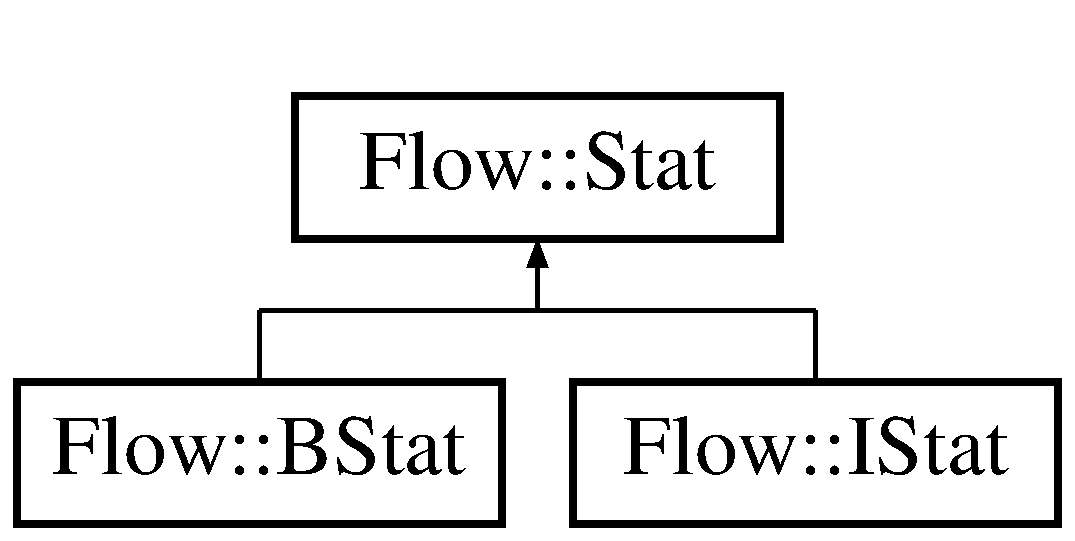
\includegraphics[height=2.000000cm]{class_flow_1_1_stat}
\end{center}
\end{figure}
\subsection*{Public Member Functions}
\begin{DoxyCompactItemize}
\item 
void \hyperlink{class_flow_1_1_stat_aecffa9e7e448ed7880a8f410cd3d96e7}{set\+Fl\+Name} (const std\+::string \&)
\item 
void \hyperlink{class_flow_1_1_stat_ab9d4b29ae4826165fea59f87b839c33e}{set\+Name} (const std\+::string \&)
\item 
std\+::string \hyperlink{class_flow_1_1_stat_a82e355b6052a2bc3433dc1f8e48204fc}{fl\+Name} () const
\item 
std\+::string \hyperlink{class_flow_1_1_stat_a3b09172b24c2ea0b6a040861b13ac16a}{name} () const
\end{DoxyCompactItemize}


\subsection{Detailed Description}


Definition at line 25 of file Stat.\+h.



\subsection{Member Function Documentation}
\hypertarget{class_flow_1_1_stat_a82e355b6052a2bc3433dc1f8e48204fc}{}\label{class_flow_1_1_stat_a82e355b6052a2bc3433dc1f8e48204fc} 
\index{Flow\+::\+Stat@{Flow\+::\+Stat}!fl\+Name@{fl\+Name}}
\index{fl\+Name@{fl\+Name}!Flow\+::\+Stat@{Flow\+::\+Stat}}
\subsubsection{\texorpdfstring{fl\+Name()}{flName()}}
{\footnotesize\ttfamily std\+::string Flow\+::\+Stat\+::fl\+Name (\begin{DoxyParamCaption}{ }\end{DoxyParamCaption}) const}



Definition at line 32 of file Stat.\+cpp.

\hypertarget{class_flow_1_1_stat_a3b09172b24c2ea0b6a040861b13ac16a}{}\label{class_flow_1_1_stat_a3b09172b24c2ea0b6a040861b13ac16a} 
\index{Flow\+::\+Stat@{Flow\+::\+Stat}!name@{name}}
\index{name@{name}!Flow\+::\+Stat@{Flow\+::\+Stat}}
\subsubsection{\texorpdfstring{name()}{name()}}
{\footnotesize\ttfamily std\+::string Flow\+::\+Stat\+::name (\begin{DoxyParamCaption}{ }\end{DoxyParamCaption}) const}



Definition at line 23 of file Stat.\+cpp.

\hypertarget{class_flow_1_1_stat_aecffa9e7e448ed7880a8f410cd3d96e7}{}\label{class_flow_1_1_stat_aecffa9e7e448ed7880a8f410cd3d96e7} 
\index{Flow\+::\+Stat@{Flow\+::\+Stat}!set\+Fl\+Name@{set\+Fl\+Name}}
\index{set\+Fl\+Name@{set\+Fl\+Name}!Flow\+::\+Stat@{Flow\+::\+Stat}}
\subsubsection{\texorpdfstring{set\+Fl\+Name()}{setFlName()}}
{\footnotesize\ttfamily void Flow\+::\+Stat\+::set\+Fl\+Name (\begin{DoxyParamCaption}\item[{const std\+::string \&}]{fl\+Name }\end{DoxyParamCaption})}



Definition at line 53 of file Stat.\+cpp.

\hypertarget{class_flow_1_1_stat_ab9d4b29ae4826165fea59f87b839c33e}{}\label{class_flow_1_1_stat_ab9d4b29ae4826165fea59f87b839c33e} 
\index{Flow\+::\+Stat@{Flow\+::\+Stat}!set\+Name@{set\+Name}}
\index{set\+Name@{set\+Name}!Flow\+::\+Stat@{Flow\+::\+Stat}}
\subsubsection{\texorpdfstring{set\+Name()}{setName()}}
{\footnotesize\ttfamily void Flow\+::\+Stat\+::set\+Name (\begin{DoxyParamCaption}\item[{const std\+::string \&}]{name }\end{DoxyParamCaption})}



Definition at line 42 of file Stat.\+cpp.



The documentation for this class was generated from the following files\+:\begin{DoxyCompactItemize}
\item 
E\+:/git/gn0mesort/\+Rothman\+Alexander\+\_\+\+C\+S\+C17\+A\+\_\+48096/proj/\+Project\+\_\+1/\+Overflow/\hyperlink{_stat_8h}{Stat.\+h}\item 
E\+:/git/gn0mesort/\+Rothman\+Alexander\+\_\+\+C\+S\+C17\+A\+\_\+48096/proj/\+Project\+\_\+1/\+Overflow/\hyperlink{_stat_8cpp}{Stat.\+cpp}\end{DoxyCompactItemize}

\chapter{File Documentation}
\hypertarget{_8dep_8inc}{}\section{Rothman\+Alexander\+\_\+\+C\+S\+C17\+A\+\_\+48096/proj/\+Project\+\_\+2/\+Overflow\+\_\+2/.dep.\+inc File Reference}
\label{_8dep_8inc}\index{Rothman\+Alexander\+\_\+\+C\+S\+C17\+A\+\_\+48096/proj/\+Project\+\_\+2/\+Overflow\+\_\+2/.\+dep.\+inc@{Rothman\+Alexander\+\_\+\+C\+S\+C17\+A\+\_\+48096/proj/\+Project\+\_\+2/\+Overflow\+\_\+2/.\+dep.\+inc}}

\hypertarget{_actor_8cpp}{}\section{E\+:/git/gn0mesort/\+Rothman\+Alexander\+\_\+\+C\+S\+C17\+A\+\_\+48096/proj/\+Project\+\_\+1/\+Overflow/\+Actor.cpp File Reference}
\label{_actor_8cpp}\index{E\+:/git/gn0mesort/\+Rothman\+Alexander\+\_\+\+C\+S\+C17\+A\+\_\+48096/proj/\+Project\+\_\+1/\+Overflow/\+Actor.\+cpp@{E\+:/git/gn0mesort/\+Rothman\+Alexander\+\_\+\+C\+S\+C17\+A\+\_\+48096/proj/\+Project\+\_\+1/\+Overflow/\+Actor.\+cpp}}
{\ttfamily \#include \char`\"{}Actor.\+h\char`\"{}}\newline
{\ttfamily \#include \char`\"{}Game.\+h\char`\"{}}\newline

\hypertarget{_actor_8h}{}\section{E\+:/git/gn0mesort/\+Rothman\+Alexander\+\_\+\+C\+S\+C17\+A\+\_\+48096/proj/\+Project\+\_\+1/\+Overflow/\+Actor.h File Reference}
\label{_actor_8h}\index{E\+:/git/gn0mesort/\+Rothman\+Alexander\+\_\+\+C\+S\+C17\+A\+\_\+48096/proj/\+Project\+\_\+1/\+Overflow/\+Actor.\+h@{E\+:/git/gn0mesort/\+Rothman\+Alexander\+\_\+\+C\+S\+C17\+A\+\_\+48096/proj/\+Project\+\_\+1/\+Overflow/\+Actor.\+h}}
{\ttfamily \#include $<$string$>$}\newline
{\ttfamily \#include $<$vector$>$}\newline
{\ttfamily \#include $<$iostream$>$}\newline
{\ttfamily \#include \char`\"{}Item.\+h\char`\"{}}\newline
{\ttfamily \#include \char`\"{}Stat.\+h\char`\"{}}\newline
{\ttfamily \#include \char`\"{}Bin\+Array.\+h\char`\"{}}\newline
\subsection*{Classes}
\begin{DoxyCompactItemize}
\item 
class \hyperlink{class_flow_1_1_actor}{Flow\+::\+Actor}
\end{DoxyCompactItemize}
\subsection*{Namespaces}
\begin{DoxyCompactItemize}
\item 
 \hyperlink{namespace_flow}{Flow}
\end{DoxyCompactItemize}
\subsection*{Enumerations}
\begin{DoxyCompactItemize}
\item 
enum \hyperlink{namespace_flow_a05bb774db920847e46f3779aaef1b07b}{Flow\+::\+Job} \{ \newline
\hyperlink{namespace_flow_a05bb774db920847e46f3779aaef1b07ba6adf97f83acf6453d4a6a4b1070f3754}{Flow\+::\+Job\+::\+None} = 0, 
\hyperlink{namespace_flow_a05bb774db920847e46f3779aaef1b07ba8c23b2b86573edf2a5ea482c2ccc1497}{Flow\+::\+Job\+::\+Knight} = 1, 
\hyperlink{namespace_flow_a05bb774db920847e46f3779aaef1b07ba88f6c01a3b5711ec2a896c9f5462497c}{Flow\+::\+Job\+::\+Cleric} = 2, 
\hyperlink{namespace_flow_a05bb774db920847e46f3779aaef1b07ba8eb9bca606e30006ccd71ab236760ce8}{Flow\+::\+Job\+::\+Mage} = 3, 
\newline
\hyperlink{namespace_flow_a05bb774db920847e46f3779aaef1b07baf7407edad1ded2d8d1e634ed49a9698e}{Flow\+::\+Job\+::\+Lancer} = 4
 \}
\end{DoxyCompactItemize}
\subsection*{Variables}
\begin{DoxyCompactItemize}
\item 
const unsigned char \hyperlink{namespace_flow_abc8632eea1ea1050e9fc2f70cba06fb8}{Flow\+::\+J\+O\+B\+\_\+\+C\+NT} = 4
\end{DoxyCompactItemize}

\hypertarget{_bin_array_8cpp}{}\section{E\+:/git/gn0mesort/\+Rothman\+Alexander\+\_\+\+C\+S\+C17\+A\+\_\+48096/proj/\+Project\+\_\+1/\+Overflow/\+Bin\+Array.cpp File Reference}
\label{_bin_array_8cpp}\index{E\+:/git/gn0mesort/\+Rothman\+Alexander\+\_\+\+C\+S\+C17\+A\+\_\+48096/proj/\+Project\+\_\+1/\+Overflow/\+Bin\+Array.\+cpp@{E\+:/git/gn0mesort/\+Rothman\+Alexander\+\_\+\+C\+S\+C17\+A\+\_\+48096/proj/\+Project\+\_\+1/\+Overflow/\+Bin\+Array.\+cpp}}
{\ttfamily \#include \char`\"{}Bin\+Array.\+h\char`\"{}}\newline

\hypertarget{_bin_array_8h}{}\section{E\+:/git/gn0mesort/\+Rothman\+Alexander\+\_\+\+C\+S\+C17\+A\+\_\+48096/proj/\+Project\+\_\+1/\+Overflow/\+Bin\+Array.h File Reference}
\label{_bin_array_8h}\index{E\+:/git/gn0mesort/\+Rothman\+Alexander\+\_\+\+C\+S\+C17\+A\+\_\+48096/proj/\+Project\+\_\+1/\+Overflow/\+Bin\+Array.\+h@{E\+:/git/gn0mesort/\+Rothman\+Alexander\+\_\+\+C\+S\+C17\+A\+\_\+48096/proj/\+Project\+\_\+1/\+Overflow/\+Bin\+Array.\+h}}
{\ttfamily \#include $<$fstream$>$}\newline
\subsection*{Classes}
\begin{DoxyCompactItemize}
\item 
class \hyperlink{class_flow_1_1_bin_array}{Flow\+::\+Bin\+Array}
\end{DoxyCompactItemize}
\subsection*{Namespaces}
\begin{DoxyCompactItemize}
\item 
 \hyperlink{namespace_flow}{Flow}
\end{DoxyCompactItemize}
\subsection*{Functions}
\begin{DoxyCompactItemize}
\item 
unsigned int \hyperlink{namespace_flow_a3fe28a3ba61421c4d80f942102b9bfdc}{Flow\+::to\+Int} (Bin\+Array \&)
\item 
std\+::string \hyperlink{namespace_flow_aecdc302d3189de5ec98c40317efedc62}{Flow\+::to\+Str} (Bin\+Array \&)
\item 
Bin\+Array \hyperlink{namespace_flow_a731bdae4bdf6527208f0a8bc3b2ab609}{Flow\+::to\+Bin} (const std\+::string \&)
\end{DoxyCompactItemize}

\hypertarget{_flags_8cpp}{}\section{E\+:/git/gn0mesort/\+Rothman\+Alexander\+\_\+\+C\+S\+C17\+A\+\_\+48096/proj/\+Project\+\_\+1/\+Overflow/\+Flags.cpp File Reference}
\label{_flags_8cpp}\index{E\+:/git/gn0mesort/\+Rothman\+Alexander\+\_\+\+C\+S\+C17\+A\+\_\+48096/proj/\+Project\+\_\+1/\+Overflow/\+Flags.\+cpp@{E\+:/git/gn0mesort/\+Rothman\+Alexander\+\_\+\+C\+S\+C17\+A\+\_\+48096/proj/\+Project\+\_\+1/\+Overflow/\+Flags.\+cpp}}
{\ttfamily \#include \char`\"{}Flags.\+h\char`\"{}}\newline

\hypertarget{_flags_8h}{}\section{E\+:/git/gn0mesort/\+Rothman\+Alexander\+\_\+\+C\+S\+C17\+A\+\_\+48096/proj/\+Project\+\_\+1/\+Overflow/\+Flags.h File Reference}
\label{_flags_8h}\index{E\+:/git/gn0mesort/\+Rothman\+Alexander\+\_\+\+C\+S\+C17\+A\+\_\+48096/proj/\+Project\+\_\+1/\+Overflow/\+Flags.\+h@{E\+:/git/gn0mesort/\+Rothman\+Alexander\+\_\+\+C\+S\+C17\+A\+\_\+48096/proj/\+Project\+\_\+1/\+Overflow/\+Flags.\+h}}
{\ttfamily \#include $<$string$>$}\newline
\subsection*{Classes}
\begin{DoxyCompactItemize}
\item 
class \hyperlink{class_flow_1_1_flg_util}{Flow\+::\+Flg\+Util}
\end{DoxyCompactItemize}
\subsection*{Namespaces}
\begin{DoxyCompactItemize}
\item 
 \hyperlink{namespace_flow}{Flow}
\item 
 \hyperlink{namespace_flow_1_1_direct}{Flow\+::\+Direct}
\item 
 \hyperlink{namespace_flow_1_1_dmg_elem}{Flow\+::\+Dmg\+Elem}
\item 
 \hyperlink{namespace_flow_1_1_diff}{Flow\+::\+Diff}
\end{DoxyCompactItemize}
\subsection*{Functions}
\begin{DoxyCompactItemize}
\item 
unsigned char \hyperlink{namespace_flow_1_1_direct_a441c0002a213a4fd71976e704ad16f33}{Flow\+::\+Direct\+::reverse} (unsigned char)
\item 
std\+::string \hyperlink{namespace_flow_1_1_direct_aab9d0fe77dd3d02485b768e5c7ccff9d}{Flow\+::\+Direct\+::to\+Str} (unsigned char)
\item 
std\+::string \hyperlink{namespace_flow_1_1_direct_a878a0d3e7b3e67a1ed1b5b15bcdac044}{Flow\+::\+Direct\+::to\+Str} (unsigned char, bool)
\item 
std\+::string \hyperlink{namespace_flow_1_1_dmg_elem_a80b9d857d3c347b4d04d852602ee0060}{Flow\+::\+Dmg\+Elem\+::to\+Str} (unsigned char)
\end{DoxyCompactItemize}
\subsection*{Variables}
\begin{DoxyCompactItemize}
\item 
const unsigned char \hyperlink{namespace_flow_1_1_direct_a3a2e55bf055fca941f5bd430389462ea}{Flow\+::\+Direct\+::\+N\+O\+NE} = 0
\item 
const unsigned char \hyperlink{namespace_flow_1_1_direct_aeaeaa2d58de609af52cf2666bf3868a7}{Flow\+::\+Direct\+::\+N\+O\+R\+TH} = 1
\item 
const unsigned char \hyperlink{namespace_flow_1_1_direct_a8ff328289a90b44b52de5251b6da59ec}{Flow\+::\+Direct\+::\+E\+A\+ST} = 2
\item 
const unsigned char \hyperlink{namespace_flow_1_1_direct_ac93371fec14643176c2413f84b02b9ad}{Flow\+::\+Direct\+::\+S\+O\+U\+TH} = 4
\item 
const unsigned char \hyperlink{namespace_flow_1_1_direct_a71884fb1eefd6b366b08e03e8eca5205}{Flow\+::\+Direct\+::\+W\+E\+ST} = 8
\item 
const unsigned char \hyperlink{namespace_flow_1_1_dmg_elem_a2c7180f371963927ddcc5b333568a33b}{Flow\+::\+Dmg\+Elem\+::\+N\+O\+NE} = 0
\item 
const unsigned char \hyperlink{namespace_flow_1_1_dmg_elem_ab1e9e2aae5dd0691b09de8ade59d3984}{Flow\+::\+Dmg\+Elem\+::\+N\+G\+H\+T\+M\+RE} = 1
\item 
const unsigned char \hyperlink{namespace_flow_1_1_dmg_elem_aa25b22e8ba30a8c765912ceda3110cab}{Flow\+::\+Dmg\+Elem\+::\+F\+I\+RE} = 2
\item 
const unsigned char \hyperlink{namespace_flow_1_1_dmg_elem_a30739bfaff89a78947afa83acd27fc16}{Flow\+::\+Dmg\+Elem\+::\+I\+CE} = 4
\item 
const unsigned char \hyperlink{namespace_flow_1_1_dmg_elem_ae77f57817a01c597933d72de6f00df36}{Flow\+::\+Dmg\+Elem\+::\+L\+I\+G\+H\+T\+NG} = 8
\item 
const unsigned char \hyperlink{namespace_flow_1_1_dmg_elem_ab161888a4cffbc8799e450085f9411b9}{Flow\+::\+Dmg\+Elem\+::\+W\+I\+ND} = 16
\item 
const unsigned char \hyperlink{namespace_flow_1_1_dmg_elem_a9cf12825628ffbf718079827d6706619}{Flow\+::\+Dmg\+Elem\+::\+H\+O\+LY} = 32
\item 
const unsigned char \hyperlink{namespace_flow_1_1_dmg_elem_a97d51ad54a8dceed5f5f3e0e856453e1}{Flow\+::\+Dmg\+Elem\+::\+S\+H\+A\+D\+OW} = 64
\item 
const unsigned char \hyperlink{namespace_flow_1_1_dmg_elem_af91abc6a76da493ae0aab97998f10a3c}{Flow\+::\+Dmg\+Elem\+::\+H\+E\+A\+L\+I\+NG} = 128
\item 
const unsigned char \hyperlink{namespace_flow_1_1_dmg_elem_a91b40559f8ea36309d1459ae990e7737}{Flow\+::\+Dmg\+Elem\+::\+A\+B\+S\+O\+L\+UT} = 255
\item 
const unsigned char \hyperlink{namespace_flow_1_1_diff_a25211e3502f69e2908f0f7a0704a791c}{Flow\+::\+Diff\+::\+N\+O\+NE} = 0
\item 
const unsigned char \hyperlink{namespace_flow_1_1_diff_a74626099944a6e3bba9dd65249e2d1af}{Flow\+::\+Diff\+::\+E\+A\+SY} = 8
\item 
const unsigned char \hyperlink{namespace_flow_1_1_diff_a2a571fad912e041a39f438cdabb5b205}{Flow\+::\+Diff\+::\+M\+E\+D\+I\+UM} = 16
\item 
const unsigned char \hyperlink{namespace_flow_1_1_diff_afda4e2a42f3b99975b1c79d953424f59}{Flow\+::\+Diff\+::\+H\+A\+RD} = 32
\end{DoxyCompactItemize}

\hypertarget{_game_8cpp}{}\section{E\+:/git/gn0mesort/\+Rothman\+Alexander\+\_\+\+C\+S\+C17\+A\+\_\+48096/proj/\+Project\+\_\+1/\+Overflow/\+Game.cpp File Reference}
\label{_game_8cpp}\index{E\+:/git/gn0mesort/\+Rothman\+Alexander\+\_\+\+C\+S\+C17\+A\+\_\+48096/proj/\+Project\+\_\+1/\+Overflow/\+Game.\+cpp@{E\+:/git/gn0mesort/\+Rothman\+Alexander\+\_\+\+C\+S\+C17\+A\+\_\+48096/proj/\+Project\+\_\+1/\+Overflow/\+Game.\+cpp}}
{\ttfamily \#include \char`\"{}Game.\+h\char`\"{}}\newline

\hypertarget{_game_8h}{}\section{E\+:/git/gn0mesort/\+Rothman\+Alexander\+\_\+\+C\+S\+C17\+A\+\_\+48096/proj/\+Project\+\_\+1/\+Overflow/\+Game.h File Reference}
\label{_game_8h}\index{E\+:/git/gn0mesort/\+Rothman\+Alexander\+\_\+\+C\+S\+C17\+A\+\_\+48096/proj/\+Project\+\_\+1/\+Overflow/\+Game.\+h@{E\+:/git/gn0mesort/\+Rothman\+Alexander\+\_\+\+C\+S\+C17\+A\+\_\+48096/proj/\+Project\+\_\+1/\+Overflow/\+Game.\+h}}
{\ttfamily \#include $<$vector$>$}\newline
{\ttfamily \#include $<$string$>$}\newline
{\ttfamily \#include $<$fstream$>$}\newline
{\ttfamily \#include $<$iostream$>$}\newline
{\ttfamily \#include $<$cstdlib$>$}\newline
{\ttfamily \#include $<$cstdio$>$}\newline
{\ttfamily \#include $<$ctime$>$}\newline
{\ttfamily \#include $<$sstream$>$}\newline
{\ttfamily \#include \char`\"{}Actor.\+h\char`\"{}}\newline
{\ttfamily \#include \char`\"{}Room.\+h\char`\"{}}\newline
{\ttfamily \#include \char`\"{}Bin\+Array.\+h\char`\"{}}\newline
{\ttfamily \#include \char`\"{}Flags.\+h\char`\"{}}\newline
\subsection*{Classes}
\begin{DoxyCompactItemize}
\item 
class \hyperlink{class_flow_1_1_gm_rand}{Flow\+::\+Gm\+Rand}
\item 
struct \hyperlink{struct_flow_1_1_config}{Flow\+::\+Config}
\item 
struct \hyperlink{struct_flow_1_1_game}{Flow\+::\+Game}
\end{DoxyCompactItemize}
\subsection*{Namespaces}
\begin{DoxyCompactItemize}
\item 
 \hyperlink{namespace_flow}{Flow}
\end{DoxyCompactItemize}
\subsection*{Functions}
\begin{DoxyCompactItemize}
\item 
void \hyperlink{namespace_flow_aa61423790cc3ea1eb33e45bb4596042a}{Flow\+::clean\+Up} ()
\item 
void \hyperlink{namespace_flow_a37add817bd1f0f674074844aa9c71a03}{Flow\+::g\+Conf} ()
\item 
void \hyperlink{namespace_flow_a0dffd1ca59d045eb50e9cb6cb48601bd}{Flow\+::g\+M\+Opts} ()
\item 
void \hyperlink{namespace_flow_af89b31b06a629493e8b9d3797d618361}{Flow\+::init} ()
\item 
void \hyperlink{namespace_flow_a0809d9a60d22a2867e9d3ffa2a7ab9bc}{Flow\+::m\+M\+Opts} ()
\item 
void \hyperlink{namespace_flow_a99dd7c10b5db12f296dc3a25313206da}{Flow\+::play} ()
\item 
void \hyperlink{namespace_flow_a652e3e72e118566969bd80c132bd4964}{Flow\+::rd\+Txt} (const std\+::string \&)
\item 
void \hyperlink{namespace_flow_a425f80ed9b32235f33d7f38cc7798386}{Flow\+::rd\+Txt} (std\+::vector$<$ std\+::string $>$ \&, const std\+::string \&)
\item 
void \hyperlink{namespace_flow_a2d6d85749fd0dd65654b3682ad46b760}{Flow\+::w\+Conf} ()
\item 
void \hyperlink{namespace_flow_a18b4909edf24f2acafecf40e42016f98}{Flow\+::save} ()
\item 
bool \hyperlink{namespace_flow_ac0d6ec00171135acca42eea277c889a1}{Flow\+::ck\+File} (const std\+::string \&)
\item 
bool \hyperlink{namespace_flow_a43e74dfbdf28d1c009d3601ac1ca3cfd}{Flow\+::encounter} (Actor \&)
\item 
bool \hyperlink{namespace_flow_ae1a1cbd4b8bf306ff4ca29275af27bf1}{Flow\+::is\+Valid} (const std\+::vector$<$ std\+::string $>$ \&, char)
\item 
bool \hyperlink{namespace_flow_a75ea47a1fbf09512d617570cce2eeb4e}{Flow\+::load} ()
\item 
char \hyperlink{namespace_flow_aad435346322f19794b3bf501e15ada95}{Flow\+::menu} (const std\+::vector$<$ std\+::string $>$ \&, unsigned int)
\item 
unsigned int \hyperlink{namespace_flow_ab9b34b787aeb9532233f97e20c4b2bf3}{Flow\+::bin\+Pow} (unsigned int)
\item 
int \hyperlink{namespace_flow_aaa39f5888b9d17b0fc04dda6c45456b6}{Flow\+::i\+Menu} (const std\+::vector$<$ std\+::string $>$ \&, unsigned int)
\item 
int \hyperlink{namespace_flow_ae3e1a43d90e5f89f9ea0e5810a499d2b}{Flow\+::to\+Int} (unsigned char)
\item 
std\+::string \hyperlink{namespace_flow_ac5fc50f86c5fa7345f2ef52daa16c086}{Flow\+::frmt\+Opt} (int)
\item 
std\+::string \hyperlink{namespace_flow_a6b0b50aaa0c160e4c79cfcaea58010db}{Flow\+::frmt\+Opt} (const std\+::string \&)
\item 
Actor \hyperlink{namespace_flow_abe71679482e53f77d3dabbf951405ff3}{Flow\+::create\+Char} ()
\item 
std\+::vector$<$ std\+::string $>$ $\ast$ \hyperlink{namespace_flow_ac4033be4d707677351bc7353a173c2e6}{Flow\+::g\+N\+Items} ()
\item 
std\+::vector$<$ std\+::string $>$ $\ast$ \hyperlink{namespace_flow_a3b1a019f8216981627fc188d1f0158b2}{Flow\+::g\+N\+Weaps} ()
\end{DoxyCompactItemize}

\hypertarget{_item_8cpp}{}\section{E\+:/git/gn0mesort/\+Rothman\+Alexander\+\_\+\+C\+S\+C17\+A\+\_\+48096/proj/\+Project\+\_\+1/\+Overflow/\+Item.cpp File Reference}
\label{_item_8cpp}\index{E\+:/git/gn0mesort/\+Rothman\+Alexander\+\_\+\+C\+S\+C17\+A\+\_\+48096/proj/\+Project\+\_\+1/\+Overflow/\+Item.\+cpp@{E\+:/git/gn0mesort/\+Rothman\+Alexander\+\_\+\+C\+S\+C17\+A\+\_\+48096/proj/\+Project\+\_\+1/\+Overflow/\+Item.\+cpp}}
{\ttfamily \#include \char`\"{}Item.\+h\char`\"{}}\newline
{\ttfamily \#include \char`\"{}Game.\+h\char`\"{}}\newline

\hypertarget{_item_8h}{}\section{E\+:/git/gn0mesort/\+Rothman\+Alexander\+\_\+\+C\+S\+C17\+A\+\_\+48096/proj/\+Project\+\_\+1/\+Overflow/\+Item.h File Reference}
\label{_item_8h}\index{E\+:/git/gn0mesort/\+Rothman\+Alexander\+\_\+\+C\+S\+C17\+A\+\_\+48096/proj/\+Project\+\_\+1/\+Overflow/\+Item.\+h@{E\+:/git/gn0mesort/\+Rothman\+Alexander\+\_\+\+C\+S\+C17\+A\+\_\+48096/proj/\+Project\+\_\+1/\+Overflow/\+Item.\+h}}
{\ttfamily \#include $<$sstream$>$}\newline
{\ttfamily \#include \char`\"{}Flags.\+h\char`\"{}}\newline
{\ttfamily \#include \char`\"{}Bin\+Array.\+h\char`\"{}}\newline
\subsection*{Classes}
\begin{DoxyCompactItemize}
\item 
class \hyperlink{class_flow_1_1_item}{Flow\+::\+Item}
\end{DoxyCompactItemize}
\subsection*{Namespaces}
\begin{DoxyCompactItemize}
\item 
 \hyperlink{namespace_flow}{Flow}
\end{DoxyCompactItemize}
\subsection*{Enumerations}
\begin{DoxyCompactItemize}
\item 
enum \hyperlink{namespace_flow_ab521722c5aec75faa5be9c5ccfff33d6}{Flow\+::\+Itm\+Type} \{ \hyperlink{namespace_flow_ab521722c5aec75faa5be9c5ccfff33d6a6adf97f83acf6453d4a6a4b1070f3754}{Flow\+::\+Itm\+Type\+::\+None} = 0, 
\hyperlink{namespace_flow_ab521722c5aec75faa5be9c5ccfff33d6af7f5d540f521d6d642502a9d459e7b16}{Flow\+::\+Itm\+Type\+::\+Potion} = 1, 
\hyperlink{namespace_flow_ab521722c5aec75faa5be9c5ccfff33d6ac77a8030f463c2c14aebd6452fc9f0a8}{Flow\+::\+Itm\+Type\+::\+Armor} = 2, 
\hyperlink{namespace_flow_ab521722c5aec75faa5be9c5ccfff33d6a18c83669920215a818638ad0e5421e4b}{Flow\+::\+Itm\+Type\+::\+Weapon} = 3
 \}
\end{DoxyCompactItemize}
\subsection*{Variables}
\begin{DoxyCompactItemize}
\item 
const unsigned char \hyperlink{namespace_flow_a185ca6f187c8d738b91552fe9a987dc6}{Flow\+::\+I\+T\+M\+\_\+\+C\+NT} = 3
\end{DoxyCompactItemize}

\hypertarget{main_8cpp}{}\section{E\+:/git/gn0mesort/\+Rothman\+Alexander\+\_\+\+C\+S\+C17\+A\+\_\+48096/proj/\+Project\+\_\+1/\+Overflow/main.cpp File Reference}
\label{main_8cpp}\index{E\+:/git/gn0mesort/\+Rothman\+Alexander\+\_\+\+C\+S\+C17\+A\+\_\+48096/proj/\+Project\+\_\+1/\+Overflow/main.\+cpp@{E\+:/git/gn0mesort/\+Rothman\+Alexander\+\_\+\+C\+S\+C17\+A\+\_\+48096/proj/\+Project\+\_\+1/\+Overflow/main.\+cpp}}
{\ttfamily \#include $<$iostream$>$}\newline
{\ttfamily \#include \char`\"{}Game.\+h\char`\"{}}\newline
\subsection*{Functions}
\begin{DoxyCompactItemize}
\item 
int \hyperlink{main_8cpp_a3c04138a5bfe5d72780bb7e82a18e627}{main} (int argc, char $\ast$$\ast$argv)
\end{DoxyCompactItemize}


\subsection{Function Documentation}
\hypertarget{main_8cpp_a3c04138a5bfe5d72780bb7e82a18e627}{}\label{main_8cpp_a3c04138a5bfe5d72780bb7e82a18e627} 
\index{main.\+cpp@{main.\+cpp}!main@{main}}
\index{main@{main}!main.\+cpp@{main.\+cpp}}
\subsubsection{\texorpdfstring{main()}{main()}}
{\footnotesize\ttfamily int main (\begin{DoxyParamCaption}\item[{int}]{argc,  }\item[{char $\ast$$\ast$}]{argv }\end{DoxyParamCaption})}



Definition at line 26 of file main.\+cpp.


\hypertarget{_room_8cpp}{}\section{E\+:/git/gn0mesort/\+Rothman\+Alexander\+\_\+\+C\+S\+C17\+A\+\_\+48096/proj/\+Project\+\_\+1/\+Overflow/\+Room.cpp File Reference}
\label{_room_8cpp}\index{E\+:/git/gn0mesort/\+Rothman\+Alexander\+\_\+\+C\+S\+C17\+A\+\_\+48096/proj/\+Project\+\_\+1/\+Overflow/\+Room.\+cpp@{E\+:/git/gn0mesort/\+Rothman\+Alexander\+\_\+\+C\+S\+C17\+A\+\_\+48096/proj/\+Project\+\_\+1/\+Overflow/\+Room.\+cpp}}
{\ttfamily \#include \char`\"{}Room.\+h\char`\"{}}\newline
{\ttfamily \#include \char`\"{}Game.\+h\char`\"{}}\newline

\hypertarget{_room_8h}{}\section{E\+:/git/gn0mesort/\+Rothman\+Alexander\+\_\+\+C\+S\+C17\+A\+\_\+48096/proj/\+Project\+\_\+1/\+Overflow/\+Room.h File Reference}
\label{_room_8h}\index{E\+:/git/gn0mesort/\+Rothman\+Alexander\+\_\+\+C\+S\+C17\+A\+\_\+48096/proj/\+Project\+\_\+1/\+Overflow/\+Room.\+h@{E\+:/git/gn0mesort/\+Rothman\+Alexander\+\_\+\+C\+S\+C17\+A\+\_\+48096/proj/\+Project\+\_\+1/\+Overflow/\+Room.\+h}}
{\ttfamily \#include $<$iostream$>$}\newline
{\ttfamily \#include $<$iomanip$>$}\newline
{\ttfamily \#include $<$sstream$>$}\newline
{\ttfamily \#include \char`\"{}Flags.\+h\char`\"{}}\newline
\subsection*{Classes}
\begin{DoxyCompactItemize}
\item 
struct \hyperlink{struct_flow_1_1_point}{Flow\+::\+Point}
\item 
class \hyperlink{class_flow_1_1_room}{Flow\+::\+Room}
\item 
class \hyperlink{class_flow_1_1_floor}{Flow\+::\+Floor}
\end{DoxyCompactItemize}
\subsection*{Namespaces}
\begin{DoxyCompactItemize}
\item 
 \hyperlink{namespace_flow}{Flow}
\end{DoxyCompactItemize}
\subsection*{Enumerations}
\begin{DoxyCompactItemize}
\item 
enum \hyperlink{namespace_flow_a01e62c2d0a9c24924a2fce4b667dd9d8}{Flow\+::\+Rm\+Event} \{ \hyperlink{namespace_flow_a01e62c2d0a9c24924a2fce4b667dd9d8a6adf97f83acf6453d4a6a4b1070f3754}{Flow\+::\+Rm\+Event\+::\+None} = 0, 
\hyperlink{namespace_flow_a01e62c2d0a9c24924a2fce4b667dd9d8ad1e9f9f891de8f9a655739a01fbf68f0}{Flow\+::\+Rm\+Event\+::\+Encounter} = 1, 
\hyperlink{namespace_flow_a01e62c2d0a9c24924a2fce4b667dd9d8ac89bfcacd77b38e1881e345801774fea}{Flow\+::\+Rm\+Event\+::\+Treasure} = 2, 
\hyperlink{namespace_flow_a01e62c2d0a9c24924a2fce4b667dd9d8a38008dd81c2f4d7985ecf6e0ce8af1d1}{Flow\+::\+Rm\+Event\+::\+Spring} = 3
 \}
\end{DoxyCompactItemize}

\hypertarget{_stat_8cpp}{}\section{E\+:/git/gn0mesort/\+Rothman\+Alexander\+\_\+\+C\+S\+C17\+A\+\_\+48096/proj/\+Project\+\_\+1/\+Overflow/\+Stat.cpp File Reference}
\label{_stat_8cpp}\index{E\+:/git/gn0mesort/\+Rothman\+Alexander\+\_\+\+C\+S\+C17\+A\+\_\+48096/proj/\+Project\+\_\+1/\+Overflow/\+Stat.\+cpp@{E\+:/git/gn0mesort/\+Rothman\+Alexander\+\_\+\+C\+S\+C17\+A\+\_\+48096/proj/\+Project\+\_\+1/\+Overflow/\+Stat.\+cpp}}
{\ttfamily \#include \char`\"{}Stat.\+h\char`\"{}}\newline

\hypertarget{_stat_8h}{}\section{E\+:/git/gn0mesort/\+Rothman\+Alexander\+\_\+\+C\+S\+C17\+A\+\_\+48096/proj/\+Project\+\_\+1/\+Overflow/\+Stat.h File Reference}
\label{_stat_8h}\index{E\+:/git/gn0mesort/\+Rothman\+Alexander\+\_\+\+C\+S\+C17\+A\+\_\+48096/proj/\+Project\+\_\+1/\+Overflow/\+Stat.\+h@{E\+:/git/gn0mesort/\+Rothman\+Alexander\+\_\+\+C\+S\+C17\+A\+\_\+48096/proj/\+Project\+\_\+1/\+Overflow/\+Stat.\+h}}
{\ttfamily \#include $<$string$>$}\newline
\subsection*{Classes}
\begin{DoxyCompactItemize}
\item 
class \hyperlink{class_flow_1_1_stat}{Flow\+::\+Stat}
\item 
class \hyperlink{class_flow_1_1_b_stat}{Flow\+::\+B\+Stat}
\item 
class \hyperlink{class_flow_1_1_i_stat}{Flow\+::\+I\+Stat}
\end{DoxyCompactItemize}
\subsection*{Namespaces}
\begin{DoxyCompactItemize}
\item 
 \hyperlink{namespace_flow}{Flow}
\end{DoxyCompactItemize}

%--- End generated contents ---

% Index
\backmatter
\newpage
\phantomsection
\clearemptydoublepage
\addcontentsline{toc}{chapter}{Index}
\printindex

\end{document}
